\documentclass[12pt]{article}

\usepackage{sbc-template}
\usepackage{url}

\usepackage[table,xcdraw]{xcolor}

\usepackage[utf8]{inputenc} 
\usepackage[normalem]{ulem}
\useunder{\uline}{\ul}{}

\usepackage[square,sort,comma,numbers]{natbib}

\usepackage[portuguese]{babel}

%#### CONFIGURAÇÃO DE GRÁFICOS ###

\usepackage{graphicx}
%\usepackage{subcaption}
\usepackage[tight,footnotesize]{subfigure}
\usepackage{float} %mais controle sobre posicionamento de imagens
\usepackage{tikz} %para fazer desenhos
\usepackage{bchart} %para graficos em barra horizontal


\usepackage{pgfplots} %pacote grafico poderoso
\pgfplotsset{width=10cm,compat=1.9} %pacote grafico poderoso
\usepgfplotslibrary{external} %Compatibilidade grafica

%#### CONFIGURAÇÕES MATEMÁTICAS ####

\usepackage{amsfonts} 
\usepackage{amssymb} 
\usepackage{amsmath,bm,bbm} 

%#### CONFIGURAÇÕES REFERENCIAS BIBLIOGRÁFICAS ####

\usepackage{natbib}
\bibpunct{[}{]}{,}{a}{,}{,}

%#### CONFIGURAÇÕES EXTRAS GERAIS ####

\usepackage{multicol} %Usar colunas
\usepackage{color} %%Usar cores
\usepackage{lipsum}
\usepackage{hyperref}
\usepackage{url}
\usepackage{csquotes}
\usepackage{array,multirow} %para gerar tabelas com colunas e/ou linhas mescladas e texto escrito na 
\usepackage{scalefnt}

\usepackage{siunitx}


\sloppy

\title{Redes de Coautoria da Base SciELO: Avaliação da Colaboração Científica por Medidas de Centralidade de Redes Complexas}

\author{Vitor Luiz Pereira Ribeiro}
  
\address{Instituto de Computação -- Universidade Federal de Alagoas
  (IC/UFAL)
  \email{vitor.ribeiro@laccan.ufal.br}
}

\begin{document} 

\maketitle

\begin{abstract}
In bibliometrics field, studies have been carried out to quantitatively and qualitatively measure the evolution of the production of scientific knowledge. In this direction, co-authorship networks is one way of indicating the interaction between authors, through the collaborative effort between people, institutions and countries for the production and publication of a scientific work. This work seeks the proposition of an investigative analysis based on the index database of SciELO scientific articles, using for that purpose, properties and metrics of graph theory and complex networks, such as degree centrality, betweeness centrality and closeness centrality, proposing a evaluation of the global co-authoship network of the Federal Universities of Brazil and the local network, defined as focal point at the Federal University of Alagoas, for a time series from 2008 to 2017 in the area of Health Sciences. 
\end{abstract}
     
\begin{resumo} 
Na área de bibliometria, estudos vêm sendo realizados para mensurar quantitativa e qualitativamente a evolução da produção do conhecimento científico. Nesta direção, as redes de coautoria é uma das formas de indicar a interação entre autores, pelo esforço colaborativo entre pessoas, instituições e países para a geração e publicação de um trabalho científico. Este trabalho busca a propositura de uma análise investigativa a partir de base de dados de indexação de artigos científico SciELO, utilizando para tal, propriedades e métricas da teoria dos grafos e redes complexas, tais como \textit{degree centrality, betweeness centrality e closeness centrality}, propondo uma avaliação da rede global de coautoria das Universidades Federais do Brasil e da rede local, definida como vértice focal a Universidade Federal de Alagoas, para série temporal de 2008 à 2017 na área de \textit{Health Sciences} - Ciências da Saúde.
\end{resumo}


\section{Introdução}

\subsection{\textbf{Definição do Problema}}

A colaboração científica é um fenômeno social que tem  por objeto a produção de conhecimento e os cientistas como os principais atores. As redes de coautoria é uma das formas de mensuração e indicação da interação entre esses atores, pelo esforço colaborativo entre pessoas, instituições e países para a geração e publicação de um trabalho científico.

Nos últimos anos vários estudos tem sido realizado para a compreensão deste fenômeno \citep{Maia2008}, buscando entender como ocorre. 
Avançar nos estudos e no entendimento da colaboração científica no Brasil é fundamental para que tenhamos uma ideia mais clara de como este fenômeno vem acontecendo na comunidade científica brasileira, possibilitando a definição e o direcionamento de políticas científicas mais adequadas \cite{Vanz2010}.

O Conselho Nacional de Desenvolvimento Científico e Tecnológico -- CNPq\footnote{http//www.cnpq.br} é o mantenedor da base de Currículos Lattes\footnote{http://lattes.cnpq.br}, a principal fonte de registro dos trabalhos e publicação científica do país. 
Entretanto, a plataforma Lattes não vem apresentando avanços significativos, principalmente pela não disponibilização de dados abertos, assim, impossibilitando a realização de pesquisas que possam descrever o comportamento bibliométrico da ciência no país.
Uma evidência da desatualização do Lattes é a própria plataforma Painel Lattes\footnote{http://estatico.cnpq.br/painelLattes/} que não possui dados atualizados.

A Scientific Electronic Library Online -- SciELO\footnote{http://www.scielo.br} é uma biblioteca eletrônica criada em 1998.
Ela realiza a indexação de um conjunto de periódicos visando o desenvolvimento de uma metodologia comum para a preparação, armazenamento, disseminação e avaliação de literatura científica em formato eletrônico.

No entanto, apesar dos esforços da SciELO em disponibilizar uma ferramenta para o maior conhecimento de métricas biliométricas e a observação do comportamento da colaboração científica, sua plataforma SciELO Analytics\footnote{http://analytics.scielo.br} ainda carece de funcionalidades para a visualização de redes de coautoria, considerando o aspecto interinstituicional.

Diante do contexto supra explanado, essa pesquisa visa a proposta de um modelo da avaliação da colaboração científica com base na análise de redes de couatorias interinstituições do Brasil. 
Buscamos responder precipualmente as seguintes questões:
\begin{itemize}
\item Como se caracterizam as redes de coautoria na base SciELO?
\item Quais as propriedades e métricas que indicam a evolução das redes de coautoria ao longo do tempo?
\item Como se observa as comunidades de colaboração científica a partir das redes de coautoria?
\end{itemize}

\subsection{\textbf{Revisão da Literatura}}

A bibliometria é uma campo de conhecimento multidisciplinar com origem na biblioteconomia e na ciência da informação, que aplica métodos estatísticos e matemáticos para analisar e construir indicadores sobre a dinâmica e evolução da informação científica e tecnológica de determinadas disciplinas, áreas, organizações ou países.

\cite{pritchard1969statistical} descrevem que bibliometria é o tratamento quantitativo das propriedades da escríta científica publicada e do comportamento que lhe é inerente. 
%%% ACF A frase que segue não faz sentido
\cite{osareh1996bibliometrics} define a biliometria como o estudo dos padrões das publicações científicas aplicando análises quantitativas e estatísticas. %Lancaster (1977: 353)% 
%%% VLR frase rescrita 

Estudos e análises bibliométricas podem ser empregadas a diversas áreas do conhecimentos com abordagens como avaliação da produtividade científica, análise de citações e cocitações, redes de coautoria, análise de fatores de impacto, dentre outros. A bibliometria possui estreitas relações com as áreas de cienciometria (ou cientometria), infometria, webometria, patentometria, e altmetria.

Para \cite{barabasi2002evolution} estudar redes de coautoria é interessante porque permite determinar como o campo de pesquisa está evoluindo e fazer previsões sobre a direção desse campo e onde os avanços terão maiores probabilidades de ocorrerem. Por outro lado, em outra obra de \cite{Barabasi2001} reconhecem que em redes de coautoria \textit{(co-authorship network)}, estudos vêm apresentando evoluções significativas, entretanto de maneira muito fragmentada, se concentrando em uma característica da rede por vez. 
Os autores ressaltam também a complexidade envolvida em virtude da velocidade de crescimento das redes, comparando-as como o comportamento da rede \textit{World Wide Web}, visto que há de se considerar os vários formatos das bases de dados e suas indexações. Fica, assim, configurado o desafio para estudos relacionados a este tema.

\subsection{\textbf{Contribuições}}
  
Neste trabalho propomos desenvolver um estudo para avaliação da colaboração científica por meio de redes de coautoria, com as seguintes caraterísticas:

\begin{itemize}
\item Reprodutibilidade com a definição da instituição vértice de referência.
\item Definição do intervalo temporal em anos para análises comparativas.
\item Explanar as características e métricas quantitativas das redes pelo aspecto da colaboração científica.
\end{itemize}

\subsection{\textbf{Objetivos}}

O objetivo desta pesquisa é a proposta da criação de um estudo modelo avaliativo do comportamento das redes de coautoria na base de dados objeto desse estudo, considerando alguns objetivos secundários, são eles:

\begin{itemize}
\item Avaliação das propriedades e indicadores de redes de coautoria inter instituição.
\item Visualização por comunidades definidas pelas regiões geográficas do Brasil.
\item Caracterização da colaboração a partir dos resultados de métricas bibliométricas de redes de coautoria.
\end{itemize}

\section{Fundamentação Teórica}

A fundamentação deste trabalho encontra-se respaldado na teoria dos grafos, na análise de redes sociais e medidas de centralidade de redes complexas. 


\subsection{Teoria dos Grafos}

Em teoria de grafos, temos que um grafo é o conjunto de $G = (\bm V,\bm E)$ ($G$ = Grafos, $V$ = Vértices e $E$ = Arestas), onde $V$ é um conjunto não vazio de objetos denominados vértices (ou nós) e $E$ é um subconjunto de pares não ordenados de $V$. Neste entendimento temos que grafos pode serem caracterizados no prisma de algumas propriedades, como por exemplo o comportamento da ligação das arestas pode ser classificado como não direcional ou direcional, onde cada aresta $\Vec E$ de $\Vec G = (\bm V,\bm \Vec E)$ possui um sentido ou orientação definido por um par ordenado $(\bm x_{1}, \bm x_{2})$, sendo $x_{1}$ o ponto inicial e $x_{2}$ o ponto final da aresta em questão.

O estudo de redes complexas é um tema  que abrange diversas áreas de conhecimento, tais como a ciência da computação, matemática, física, biologia e sociologia. 
O termo ``redes complexas'' refere-se a um grafo que apresenta uma estrutura topográfica não trivial, composto por um conjunto de vértices (nós) que são interligados por meio de arestas \cite{barabasi2003everything}. 
O estudo de redes na forma de grafos é um dos pilares da matemática discreta e teve início em 1735, quando Euler propôs uma solução para o problema das pontes de Königsberg, originando a teoria dos grafos.

Redes de coautoria se caracteriza por ligação não direcional, ou seja, que independe de quem seja o ponto de origem para o destino da ligação, pois devemos para a proposta deste trabalho, considerar que se uma instituição publicou um artigo em coautoria com outra instituição, a recíproca é verdadeira e não há distinção de qual tem propriedades valoradas, como a iniciativa ou mesmo o grau de participação do coautor na publicação em tela.

As figuras abaixo representam a plotagem de grafos apresentando a visão da abordagem de coautorias intra-regional conforme a Figura~\ref{grafo1}, e coautorias inter-regional vide Figura~\ref{grafo2}, onde $S$ é a representação da região da instituição, $X$ os autores (vértices ou nós) e as arestas/ligações representam a relação de coautoria entre eles.


\begin{figure}[H]
\centering
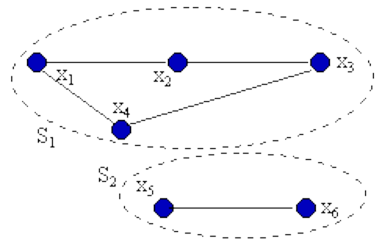
\includegraphics[scale=0.8]{images/intra-grafo.pdf}
\caption{Grafo com representação de Rede de Coautoria intra grupos}
\label{grafo1}
\end{figure}

\begin{figure}[H]
\centering
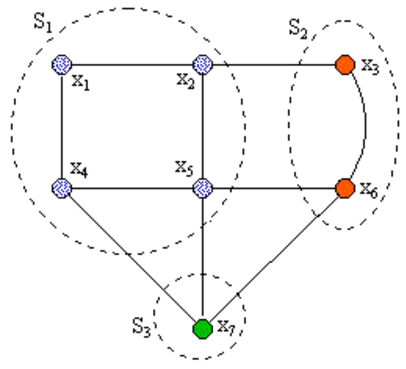
\includegraphics[scale=0.8]{images/inter-grafo.pdf}
\caption{Grafo com representação de Rede de Coautoria inter grupos}
\label{grafo2}
\end{figure}

\subsection{Análise de Redes Sociais}

Conforme \cite{Silva2006}, a análise de redes sociais interessa a pesquisadores de vários campos do conhecimento que, na tentativa de compreender o seu impacto sobre a vida social, deram origem a diversas metodologias de análise que têm como base as relações entre os indivíduos, em uma estrutura em forma de redes.

A análise de redes sociais (ARS ou SNA, da expressão em inglês \textit{Social Network Analysis)} é uma abordagem oriunda da sociologia, da psicologia social e da antropologia. \cite{freeman1996some,wasserman1994social}. ARS não é algo recente, há estudos, como o trabalho de \cite{otte2002social} que buscou desde a década de 1970, análises de redes de informação, de pesquisadores e de citações, como também de redes de coautoria.

 Redes de couatoria utiliza-se da análise de redes sociais embasada nas propriedades e aplicações de redes complexas, a qual vemos a seguir.


\begin{figure}[H]
\centering
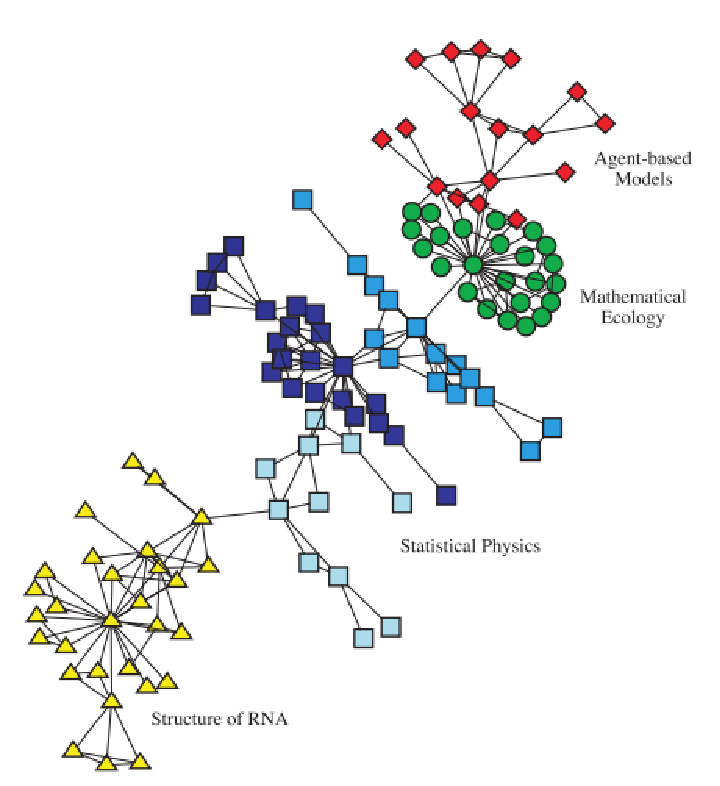
\includegraphics[scale=0.6]{images/rede-newman.pdf}
\caption{Pequena Rede de Coautoria de Newman}
\label{rede1}
\end{figure}


\subsection{Redes Complexas}

No contexto da teoria de redes complexas, uma rede corresponde a um grafo, que se representa por um conjunto de nós ligados por arestas, que em conjunto formam uma rede.  Esta rede ou grafo, permite representar relações com fundamento das propriedades dos vários tipos de grafos e como são constituídos, ou seja, como se agrupam os seus nós e são ligadas suas arestas %\cite{mendes2005fisica}.

As propriedades de redes complexas às quais utilizaremos nesse trabalho se encontram definidas a seguir.

\noindent \textbf{Definição 2.3.1} (Grau de um nó). O número de vértices adjacentes a um determinado vértice $x_i$ chama-se de grau de $x_i$. Em um grafo direcionado $\Vec G = (\bm V,\bm \Vec E)$, diferenciamos o grau de saída (output) do grau de entrada (input):

\begin{equation}
k^{out}_{x_{i}}(\Vec{G}) = \sum_{x_j \in V : x_j \neq x_i}^{} A[x_i,x_j]
\label{eq:grauOutput}
\end{equation}

\begin{equation}
k^{in}_{x_{i}}(\Vec{G}) = \sum_{x_j \in V : x_j \neq x_i}^{} A[x_j,x_i]
\label{eq:grauInput}
\end{equation}

Desse modo, chamamos de grau de $x_i$: 

\begin{equation}
k_{x_i}(\Vec{G}) = k^{out}_{x_{i}}(\Vec{G}) + k^{in}_{x_{i}}(\Vec{G})
\label{eq:grau}
\end{equation}

%\noindent \textbf{Definição 2.3.2} (Distribuição da conectividade). Consiste da forma como se distribuem as ligações pelos nós.

%\noindent \textbf{Definição 2.3.3} (Conectividade média). É definida como a média, sobre todos os pares de vértices, do número máximo de caminhos conectando dois vértices. Logo:

%\begin{equation}
%\Bar{k}(\Vec{G}) = \frac{\sum_{x_i, x_j}^{} k_{\Vec{G}}(x_i, x_j)}{{n \choose 2}}
%\label{eq:grauInput}
%\end{equation}

%Onde $k_{\Vec{G}}(x_i, x_j)$ é a conectividade entre $x_i$ e $x_j$, definida como o máximo número de ligações conectando ambos vértices e $n$ é o número de nós de $G$.

%\noindent \textbf{Definição 2.3.4} (Caminho mais curto). Consiste de qualquer caminho que ligue dois vértices $x_i$ e $x_j$ e possua a menor distância, denotada por $d_G$.

\noindent \textbf{Definição 2.3.2} (Centralidade de um nó - \textit{Degree centrality}). Definida como o número de ligações incidentes de um vértice, esta medida nos informa qual a probabilidade de um vértice receber alguma informação da rede. Logo, a centralidade de um vértice $v$ de um grafo $G = (\bm V,\bm E)$ é dada por:

\begin{equation}
    C_D(\bm v) = deg(\bm v)
\end{equation}

Uma vez que a direção das arestas podem influenciar o cálculo, em redes direcionadas existem duas medidas distintas de centralidade de grau: indegree, que corresponde ao número de ligações direcionadas para o nó e outdegree, que consiste no número de ligações que o nó encaminha para os demais vértices da rede. 

\noindent \textbf{Definição 2.3.3} (Intermediação - \textit{Betweenness centrality}). Trata-se de uma medida de centralidade de um grafo baseada em caminhos mínimos. A intermediação de um nó $v$ é dada do seguinte modo: 

\begin{equation}
    g(\bm v) = \sum_{s \neq t \neq v} \frac{\sigma_{st}(v)}{\sigma_{st}}
\end{equation}

Onde $\sigma_{st}$ é o número total de caminhos mínimos do nó $s$ para o nó $t$ e $\sigma_{st}(v)$ é o número de caminhos mínimos de $s$ para $t$ que utilizam o nó $v$ como intermediário.

 A intermediação também pode ser normalizada, sem perda de precisão, dividindo seu resultado pelo número de pares de nós não incluindo $v$, de maneira que $g(\bm v) \in [0,1]$. Tal medida é vista como mais poderosa que apenas a conectividade, uma vez que fornece uma informação mais global sobre a rede em questão.

\noindent \textbf{Definição 2.3.4} (Proximidade - \textit{Closeness Centrality}). Em um grafo conectado, a proximidade de um nó é uma medida de centralidade calculada pela inversa da soma do comprimento dos caminhos mínimos entre um dado nó $v$ e todos os demais nós do grafo. Desse modo, quanto mais central for o nó, mais próximo dos demais esse se encontrará. Sua fórmula é definida como:

\begin{equation}
    C(\bm v) = \frac{1}{\sum_{\forall u \in V, u\neq v}d_G(u,v)}
\end{equation}

Onde, $d(u,v)$ é a distância do caminho mínimo entre $u$ e $v$.

Usualmente, na literatura costuma-se usar sua versão normalizada, dada não mais pela soma de seus caminhos mínimos e sim pela média destes, como visto a seguir:

\begin{equation}
    C(\bm v) = \frac{N - 1}{\sum_{\forall u \in V, u\neq v}d_G(u,v)}
\end{equation}

Onde, $N$ é o número de nós do grafo, ou seja, $N = |V|$. Para grafos extremamente grandes a diferença $- 1$ torna-se irrelevante, podendo ser descartada.

\noindent \textbf{Definição 2.3.5} (Diâmetro). É definido como a excentricidade máxima entre dois nós. A excentricidade de um nó $x_i$ é definida como a distância máxima de $x_i$ a todos os outros nós do grafo $G$.

\noindent \textbf{Definição 2.3.6} (Coeficiente de agregação ou aglomeração - \textit{clustering coefficient}). Trata-se do número de ligações entre os vizinhos mais próximos de um nó.

\noindent \textbf{Definição 2.3.7} (Redes estáticas/dinâmicas). Uma rede é estática quando não há variação do número de nós e, é dinâmica, quando é possível modelar o seu crescimento pela análise da variação da sua estrutura ao longo do tempo.

A figura abaixo ilustra a topologogia das medidas de centralidade: a) \textit{degree centrality}; b) \textit{closeness centrality} e c) \textit{betweeness centrality}. Com elas podemos perceber por meio dos vértices de cor vermelha a disposição dos mesmos na topologia da rede, e seus respectivos posicionamaentos, nos levando a compreender o tipo da sua centralidade e seu papel na rede.

\begin{figure}[H]
\centering
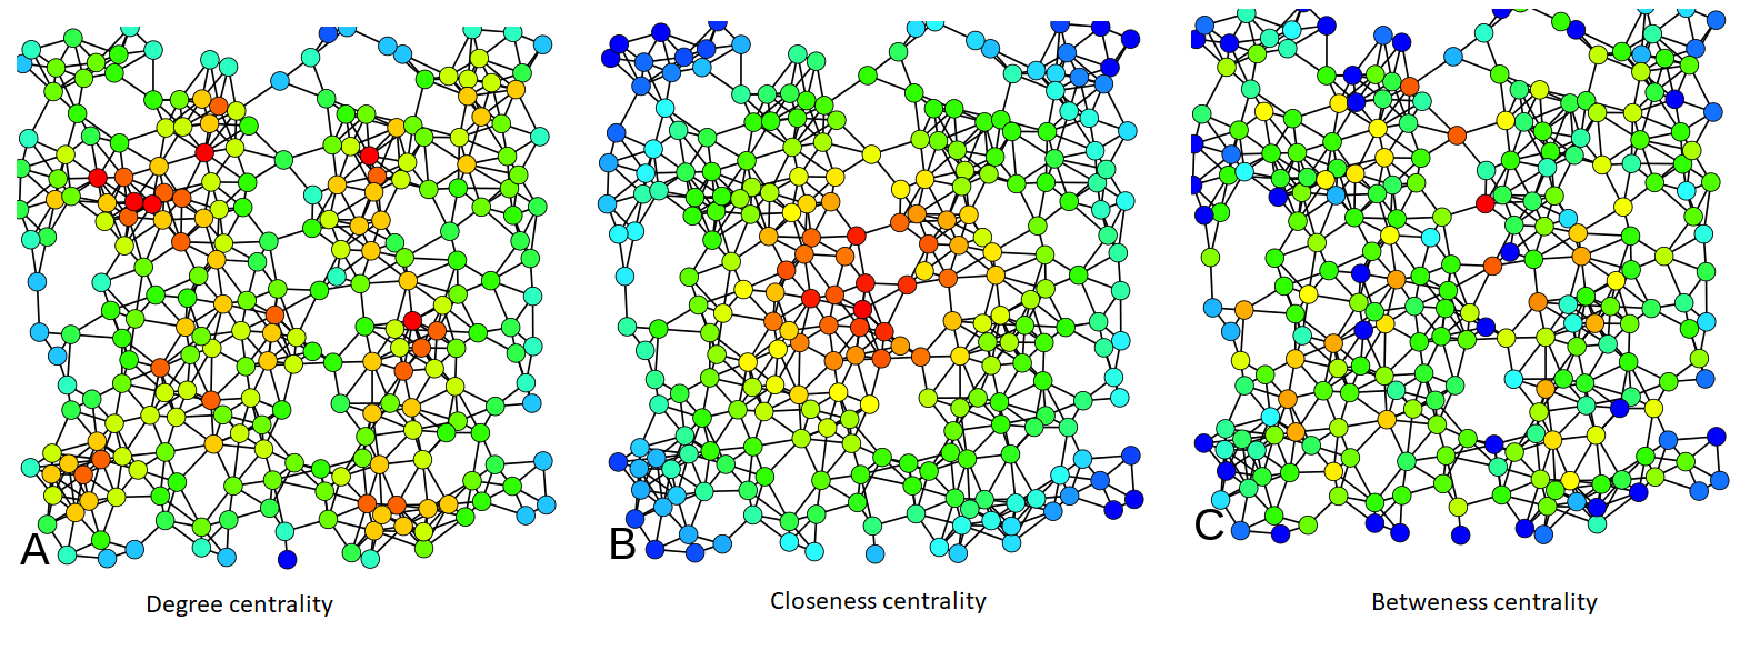
\includegraphics[scale=0.5]{images/Centrality.pdf}
\caption{Redes com ilustração das medidas de centralidade
Fonte: Claudio Rocchini - Adaptado}
\label{centrality}
\end{figure}

\section{Colaboração Científica}

Colaboração científica pode ser definida como interação que ocorre dentro de um contexto social entre dois ou mais cientistas, que facilita a partilha de significado e conclusão de tarefas em relação a um objetivo mútuo, compartilhado e organizado. Os cientistas que colaboram também podem trazer metas individuais adicionais para uma colaboração. \cite{Sonnenwald}

Ainda, segundo a autora, a colaboração ocorre dentro do contexto social da ciência, que inclui elementos como a revisão por pares, sistemas de prêmios, paradigmas científicos, políticas de ciência nacionais e internacionais, bem como normas implícitas ao campo disciplinar das instituições de pesquisa e/ou universidades. 

Conforme \cite{Newman2004}, há algum tempo se percebe que a coautoria de artigos em periódicos acadêmicos fornece uma janela sobre padrões de colaboração dentro da comunidade acadêmica. 

Para \cite{Sonnenwald}, estudos da colaboração científica está aumentando, por possuir o potencial de auxiliar a resolução de problemas científicos complexos e promover agendas políticas, econômicas e sociais. 

\section{Metodologia} 

A metodologia utilizada para a presente pesquisa utiliza um modelo exploratório que consiste em quatro etapas cíclicas: 
a)~definição da rede, 
b)~tratamentos de dados da rede; 
c)~determinação das características estruturais e 
d)~inspeção visual \cite{de2018exploratory}.

A definição da rede resultou da coleta dos dados realizada no portal da SciELO\footnote{http://static.scielo.org}. 
Foram  realizados tratamentos desses dados normalizando a padronização os campos da Unidade Federativa (UF). 
A base foi complementada pela informação da localidade geográfica associando os estados (UF) às regiões do Brasil. 
%%% ACF Escreva sempre da forma mais simples e direta possível, a seguinte frase poderia ser "Documentos de origem estrangeira foram definidos como ``Exterior''.
%% Documentos de origem estrangeira foram definidos como ``Exterior''.
%%% VLR Frase reescrita 
%%% VLR documentos do Exterior foram excluídos do escopo

Os dados foram coletados no sítio eletrônico da SciELO a partir do endereço \url{http://static.scielo.org/tabs/tabs_bra}. Os dados associam os documentos publicados em coautoria de um autor com sua respectiva instituição de origem por um ID. O conjunto de dados amostral utilizado para esta pesquisa compreende o período entre 2008 à 2017 e os documentos relacionados as Universidades Federais do país.  

Foi utilizada a linguagem de programação \texttt R, possibilitando que o resultado deste trabalho seja coberto ponta a ponta com a mesmo código, facilitando assim a reprodutibilidade desta pesquisa.

O total de documentos indexados no dados coletados resultou um montante de 1.302.659 documentos indexados, para fins desta pesquisa a amostra determinada para área de \textit{Health Sciences} o que resultou um total de 112.762 documentos.

A produção dos resultados teve por fundamento a teoria dos grafos e na análise de redes sociais, onde buscou a aplicação das métricas de redes complexas, para a compreensão do comportamento das redes de coautoria do presente estudo.

Este trabalho utilizou-se da linguagem \texttt R com o uso dos pacotes \texttt{tidyverse}, \texttt{igraph}, \texttt{ggraph} e \texttt{visNetwork}. A seguir descrevemos as etapas cíclicas proposta por \cite{de2018exploratory} para estudos relacionados ARS.

\subsection{Definição da rede}

As redes objeto de estudo desta pesquisa é a relação de coautoria existentes nos documentos indexados na base de dados da SciELO, objetivando a criação de um modelo exploratório. Foram definidas as redes de coautoria segregadas pela Unidade Federativa (UF) e Região Geográfica do Brasil para as Universidades Federais do país. Redes de coautoria são classificadas como não-direcionada, ou seja, as ligações existentes entre os vértices independem de uma orientação ou direção.

Os vértices da rede são as Unidades Federativas (UF), agrupadas pelas instituições federais às quais fazem parte da mesma, as arestas as ligações refere-se a ocorrência de coautoria entre as instituições das UF. As arestas são valoradas possuindo pesos pela frequência de ocorrência das coautorias, os vértices são ponderados pelo volume de coautorias, bem como pelos laços, ou seja, as coautorias realizadas entre instituições da mesma UF. %Para este trabalho e por fins topológicos das redes, desconsideramos os pesos para o cálculo das métricas, resultando apenas para inspeção visual das redes geradas.


\subsection{Tratamento de dados da rede}

Nesta etapa foram elaborados alguns tratamentos da rede, tal como limpeza e padronização de alguns dados, de forma mínima e minuciosa, para evitar que a reprodutibilidade reste prejudicada. Buscamos a padronização dos nomes das Unidades Federativas, e a associação de suas respectivas região geográfica.

As Universidades Federais do Brasil foram agrupadas por estados sendo representadas pelo nome no Estado (UF - Unidade Federativa). Foram realizadas rotinas de geração das matrizes e \textit{datasets} necessários aos cálculos das métricas, tal como a plotagem das redes e gráficos.

\subsection{Determinação das características estruturais}

Conforme \cite{de2018exploratory} a exploração de uma rede por suas métricas que descreve sua caracterização estrutural é uma forma mais concisa e precisa quando comparada a inspeção visual, no entanto as métricas por vezes são abstratas e de difícil interpretação. Por isso, deve-se utilizar ambas abordagens analíticas as métricas estruturais da rede e sua observação gráfica.

Foram escolhidas as métricas básicas do número de vértices e arestas, grau médio do vértice, diâmetro da rede, e distância média, centralidade do grau, centralidade de proximidade, e centralidade de intemediação, que foram aplicadas ao período em análise de 2008 à 2017 para a àrea de \text{Health Science}. As métricas aferidas denotam de forma quantitativa o comportamento da colaboração científica com bases nas redes de coautoria geradas.

\subsection{Inspeção visual}

Uma forma enriquecedora de análise de redes sociais é a observação gráfica, para isso são gerados gráficos das redes para representar suas relações e permitir por análise visual a o conhecimento da dinâmica existente pela disposição dos vértices e arestas.

Primeiramente insta ressaltar que no estudos iniciais e exploratórios da base SciELO foram encontradas diversos tipos de instituições de ensino e pesquisa, e que para o objeto do estudo deste trabalho os escopos das redes foram definidos pelas coautorias existentes entre as Universidades Federais do país em suas respectivas Unidades Federativas (UF). 

A análise das redes de coautoria consistiu em uma perspectiva regional explorando suas propriedades e caraterísticas. Foram definidos a área de \textit{Health Sciences} e o período compreendido entre 2008 à 2017, considerando a rede global que consiste todas as Universidades Federais do Brasil agrupadas pelo Estado (UF - Unidade Federativa) a que correspondem. E outra rede tendo como vértice local (ou focal) a Unidade Federativa Alagoas, de maneira a se observar a dinâmica de interação e evolução dessas redes em um prisma analítico e comparativo das redes de coautoria ao longo do tempo.

Os resultados obtidos (gráficos e númericos) permitem-nos obter um conhecimento descritivo das interações existentes na relação de coautoria entre as relaçõe de coautorias estudas da base SciELO. No aspecto gráfico as arestas possuem espessuras maior ou menor de acordo com o peso definido pelo número de publicações em coautoria, assim, as UF que possuem interações mais fortes ou mais fracas. 

Os vértices foram definidos de um mesmo tom de cor para representar a região geográfica do páis a qual pertence a UF, a espessura do laço do vértice detona também o volume de coautorias realizadas dentro da mesma UF.

\section{Resultados}

Com a aplicação dos métodos explanados e a fundamentação teórica utilizada, apresentamos os resultados, contextualizando com o problema central deste trabalho e objetivos percutidos. 

Na primeira parte, apresentamos os resultados topológicos da rede, pelo seu número de vértice e arestas, onde é observado que a variação de vértices é pequena, em virtude da desconexão ou reconexão de um ano para o outro. Os vértices da rede consiste em 27, sendo 26 UF - Estados e o Distrito Federal. Conforme gráfico apresentado o número de ligações (arestas) entre os vértices foi crescente.

Na segunda parte, as redes de coautorias são apresentadas em forma de mosaico para fins de inspeção visual, observando então a sua evolução e dinâmica no período analisado.

Na terceira parte, é apresentado o cálculo das medidas de centralidade utilizadas neste trabalho, com a apresentação dos gráficos comparativos entre o posicionamento da Universidade Federal de Alagoas, quando comparada de forma analítica em relação ao comportamento ds rede e a interpretação das medidas médias das Universidades Federais do Brasil.

\begin{table}[H]
\begin{tabular}{@{}lcccccccccc@{}}
\rowcolor[HTML]{C0C0C0} 
\textbf{\begin{tabular}[c]{@{}l@{}}Dimensão /\\ Topologia\end{tabular}} &\textbf{2008} &\textbf{2009} &\textbf{2010} & \textbf{2011} & \textbf{2012} &\textbf{2013} &\textbf{2014} &\textbf{2015} & \textbf{2016} & \textbf{2017} \\ 
Vértices & 27 & 25 & 25 & 25 & 26 & 26 & 26 & 27 & 26 & 26\\
\rowcolor[HTML]{EFEFEF} 
Arestas & 109 & 122 & 163 & 165 & 181 & 183 & 197 & 194 & 298 & 199
\end{tabular}
\end{table}  

\begin{figure}[H]
\centering
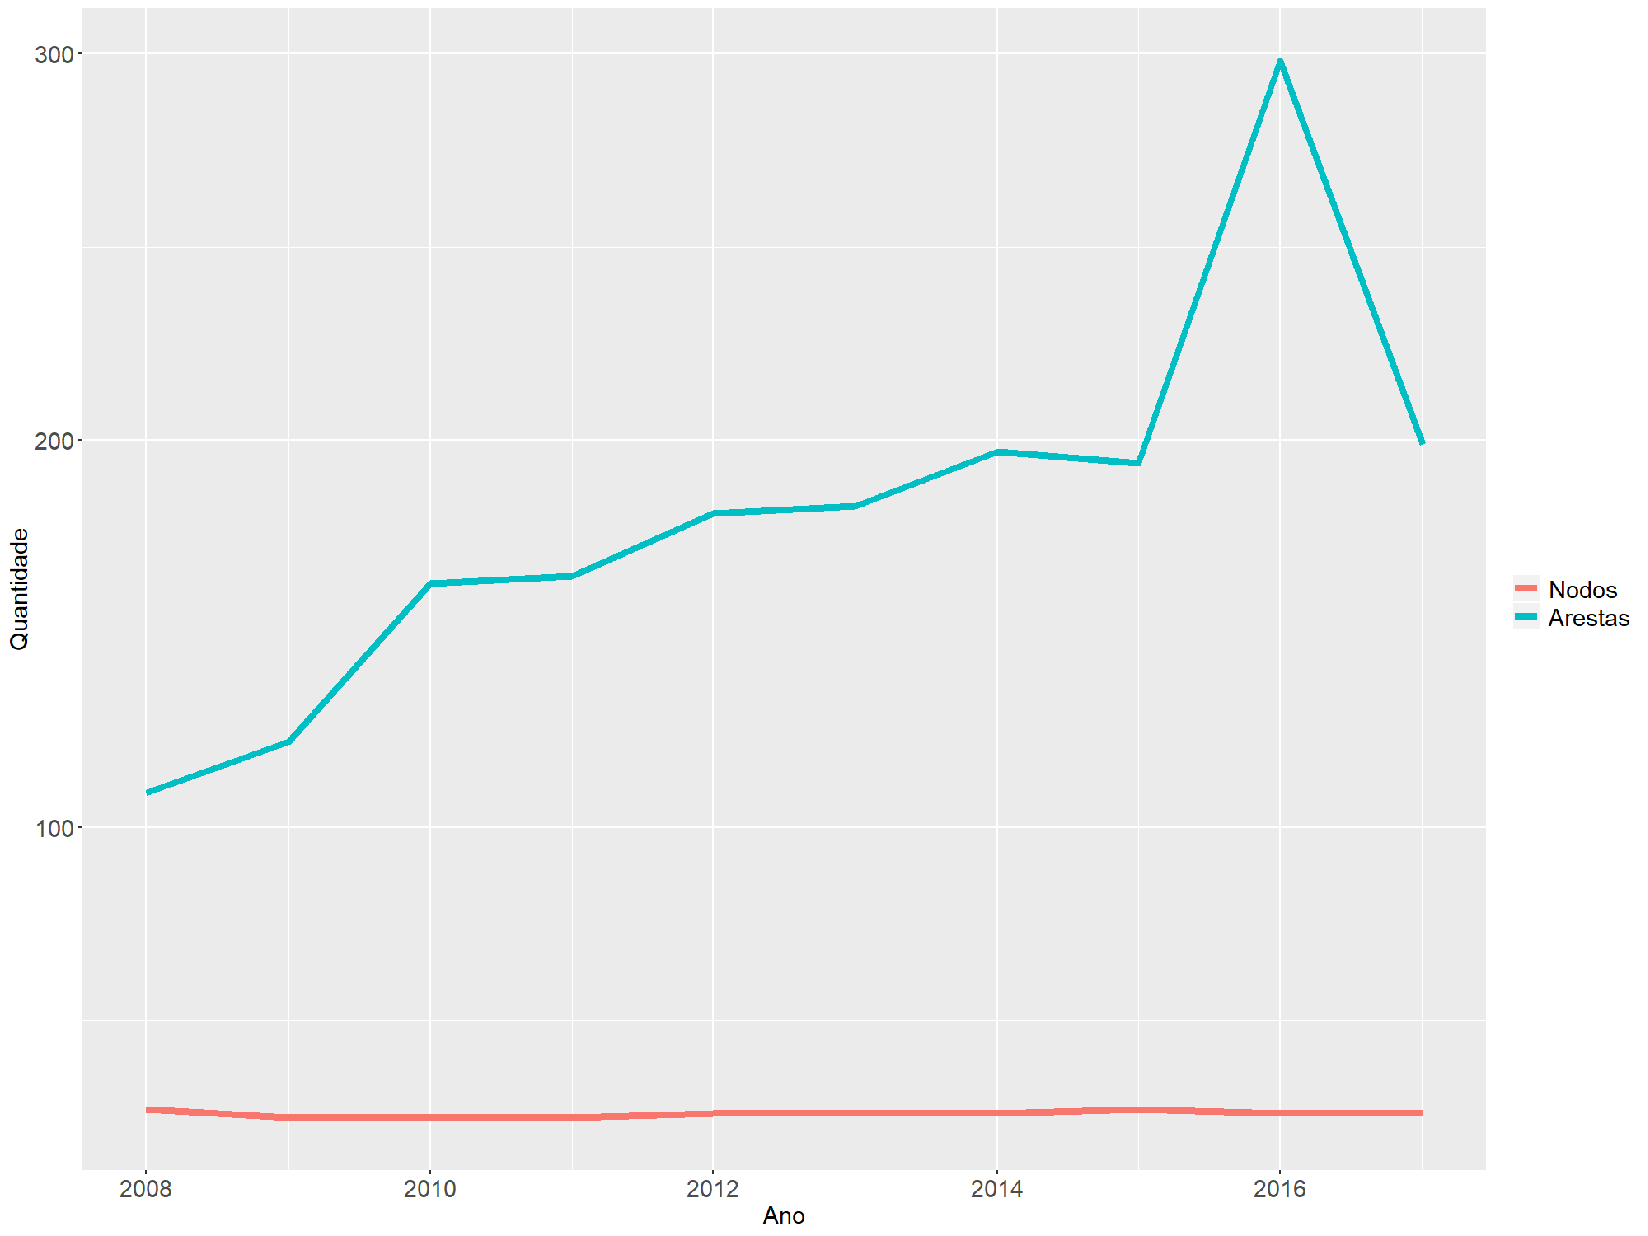
\includegraphics[scale=0.3]{images/nos-arestas.pdf}
\caption{Gráfico em Linha - Vértices e Arestas}
\label{Rede de Coautoria - UF BR 2009}
\end{figure}

Na tabela abaixo apresentamos os resultados das mensurações da densidade, tamanho, diâmetro e da aglomeração (clustering coefficient), destacando uma crescente aglomeração nos anos de 2015 e 2016. Na observação do ano de 2017 percebemos uma decrescente da densidade bem como da aglomeração, possivelmente por algum fator exogêno, como por exemplo, o não envio de artigos para indexação.

\begin{table}[H]
\begin{tabular}{@{}ccccc@{}}
\rowcolor[HTML]{C0C0C0} 
\textbf{\begin{tabular}[c]{@{}c@{}}Rede \\ Health Sciences\end{tabular}} & \textbf{Densidade} & \textbf{Tamanho} & \textbf{Diâmetro} & \textbf{\begin{tabular}[c]{@{}c@{}}Aglomeração \\ (clustering coefficient)\end{tabular}} \\ 
\rowcolor[HTML]{FFFFFF} 
\textbf{2008} & 0,121 & 27 & 3 & 0,523\\ 
\rowcolor[HTML]{EFEFEF} 
\textbf{2009} & 0,165 & 25 & 3 & 0,625\\ 
\rowcolor[HTML]{FFFFFF} 
\textbf{2010} & 0,23 & 25 & 4  & 0,726\\ 
\rowcolor[HTML]{EFEFEF} 
\textbf{2011} & 0,235 & 25 & 3 & 0,744\\
\rowcolor[HTML]{FFFFFF} 
\textbf{2012} & 0,238 & 26 & 3 & 0,773\\ 
\rowcolor[HTML]{EFEFEF} 
\textbf{2013} & 0,242 & 26 & 3 & 0,772\\ 
\rowcolor[HTML]{FFFFFF} 
\textbf{2014} & 0,265 & 26 & 3 & 0,745\\ 
\rowcolor[HTML]{EFEFEF} 
\textbf{2015} & 0,238 & 27 & 3 & 0,803\\ 
\rowcolor[HTML]{FFFFFF} 
\textbf{2016} & 0,418 & 26 & 3 & 0,943\\ 
\rowcolor[HTML]{EFEFEF} 
\textbf{2017} & 0,266 & 26 & 3 & 0,798\\ 
\end{tabular}
\end{table}

\subsection{Redes de Coautoria - Base SciELO - Health Sciences}

Apresentaremos as redes da área de \textit{Health Science} para todas as UFs, doravante Rede Brasil (das Universidades Federais) e a Rede Alagoas (para Universidade Federal de Alagoas), onde foi considerado o vértice Alagoas como ponto focal para a plotagem da rede.

As características propostas na plotagem da rede é, formato em círculo para fins comparativos, disposição dos vértices com coloração das UF pertencentes a mesma região geográfica, espessura e coloração das arestas indicando o maior volume/peso das coautorias existente entre as UFs, espessuras dos laços, indicando peso das coautorias existentes na mesma UF.

\subsubsection{Rede de Coautoria das Universidade Federais do Brasil}

A rede de coautoria das Universidades Federais do Brasil é composta de 27 vértices da rede e suas ligações representando as coautorias existentes. Nessa inspesação podemos observa o aumento da densidade da rede e o aumento da conectividade, notando o maior número de vértices ligados e o aumento de arestas.

%\begin{figure}[H]
%\centering
%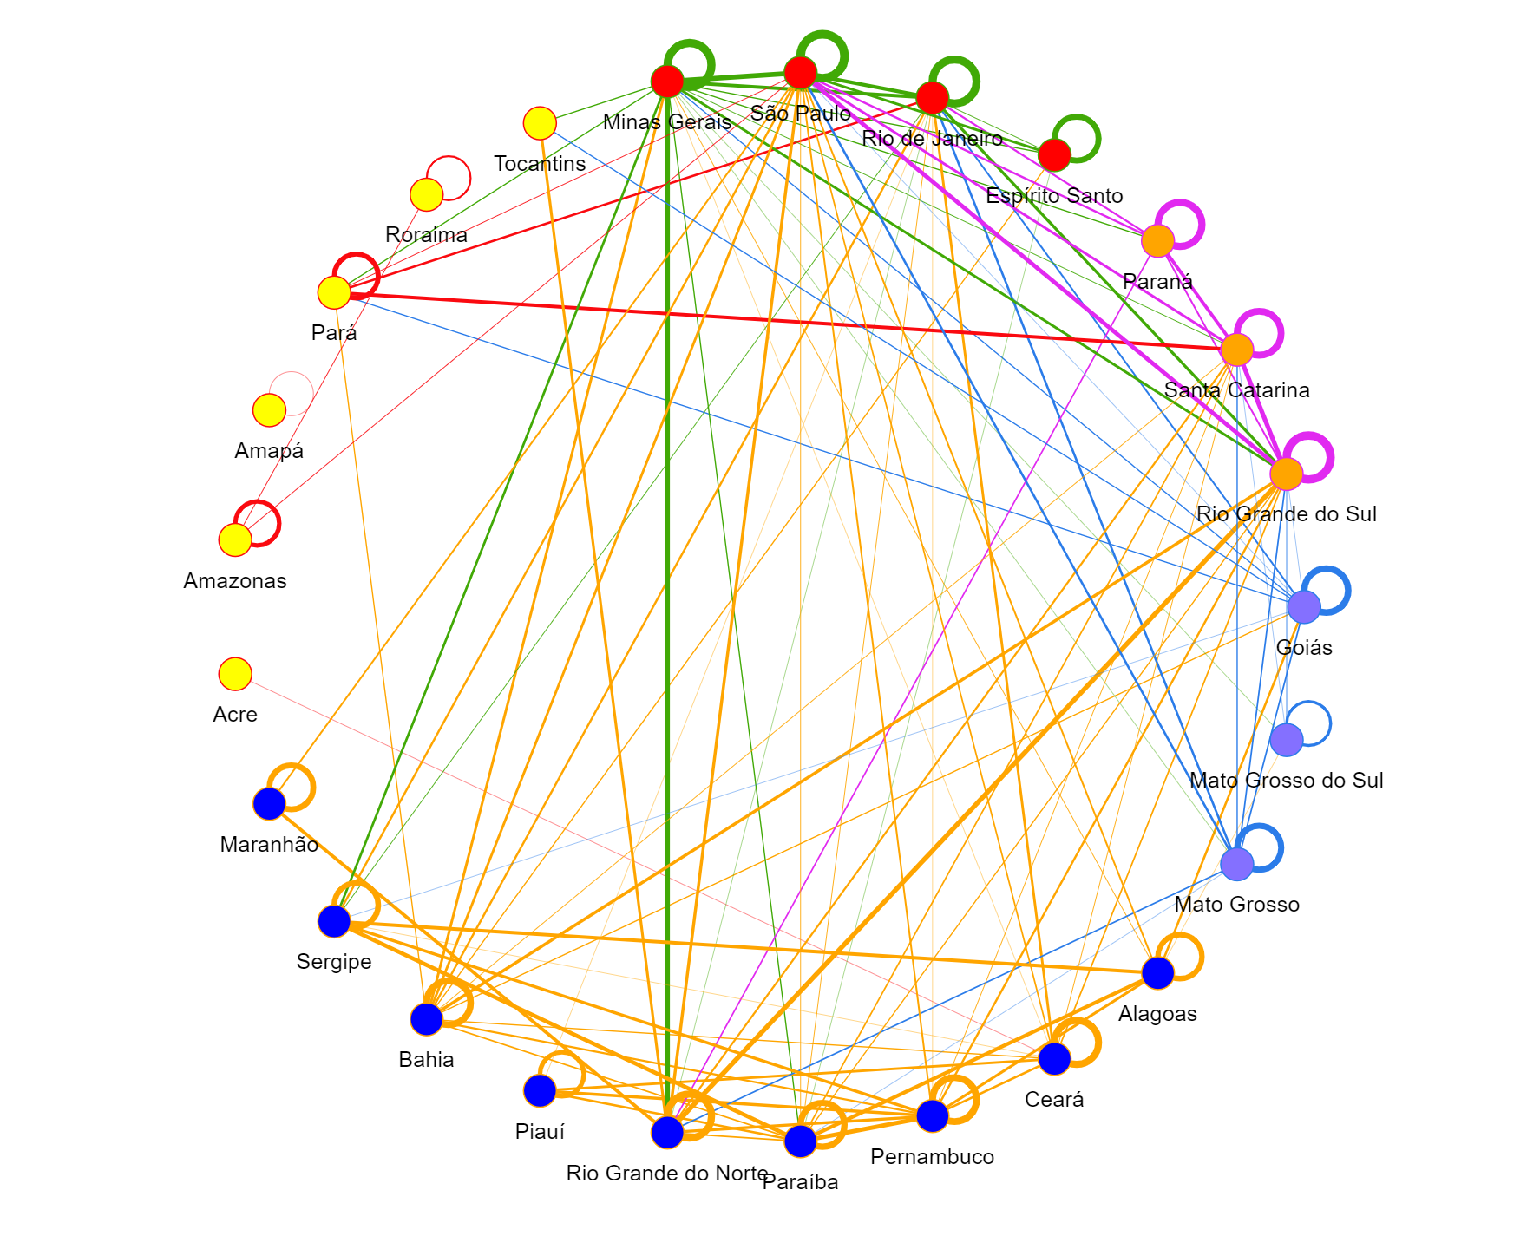
\includegraphics[scale=0.6]{images/rede-2009.pdf}
%\caption{Rede de Coautoria das Universidades Federais do Brasil - 2009}
%\label{Rede de Coautoria - UF BR 2009}
%\end{figure}

%\begin{figure}[H]
%\centering
%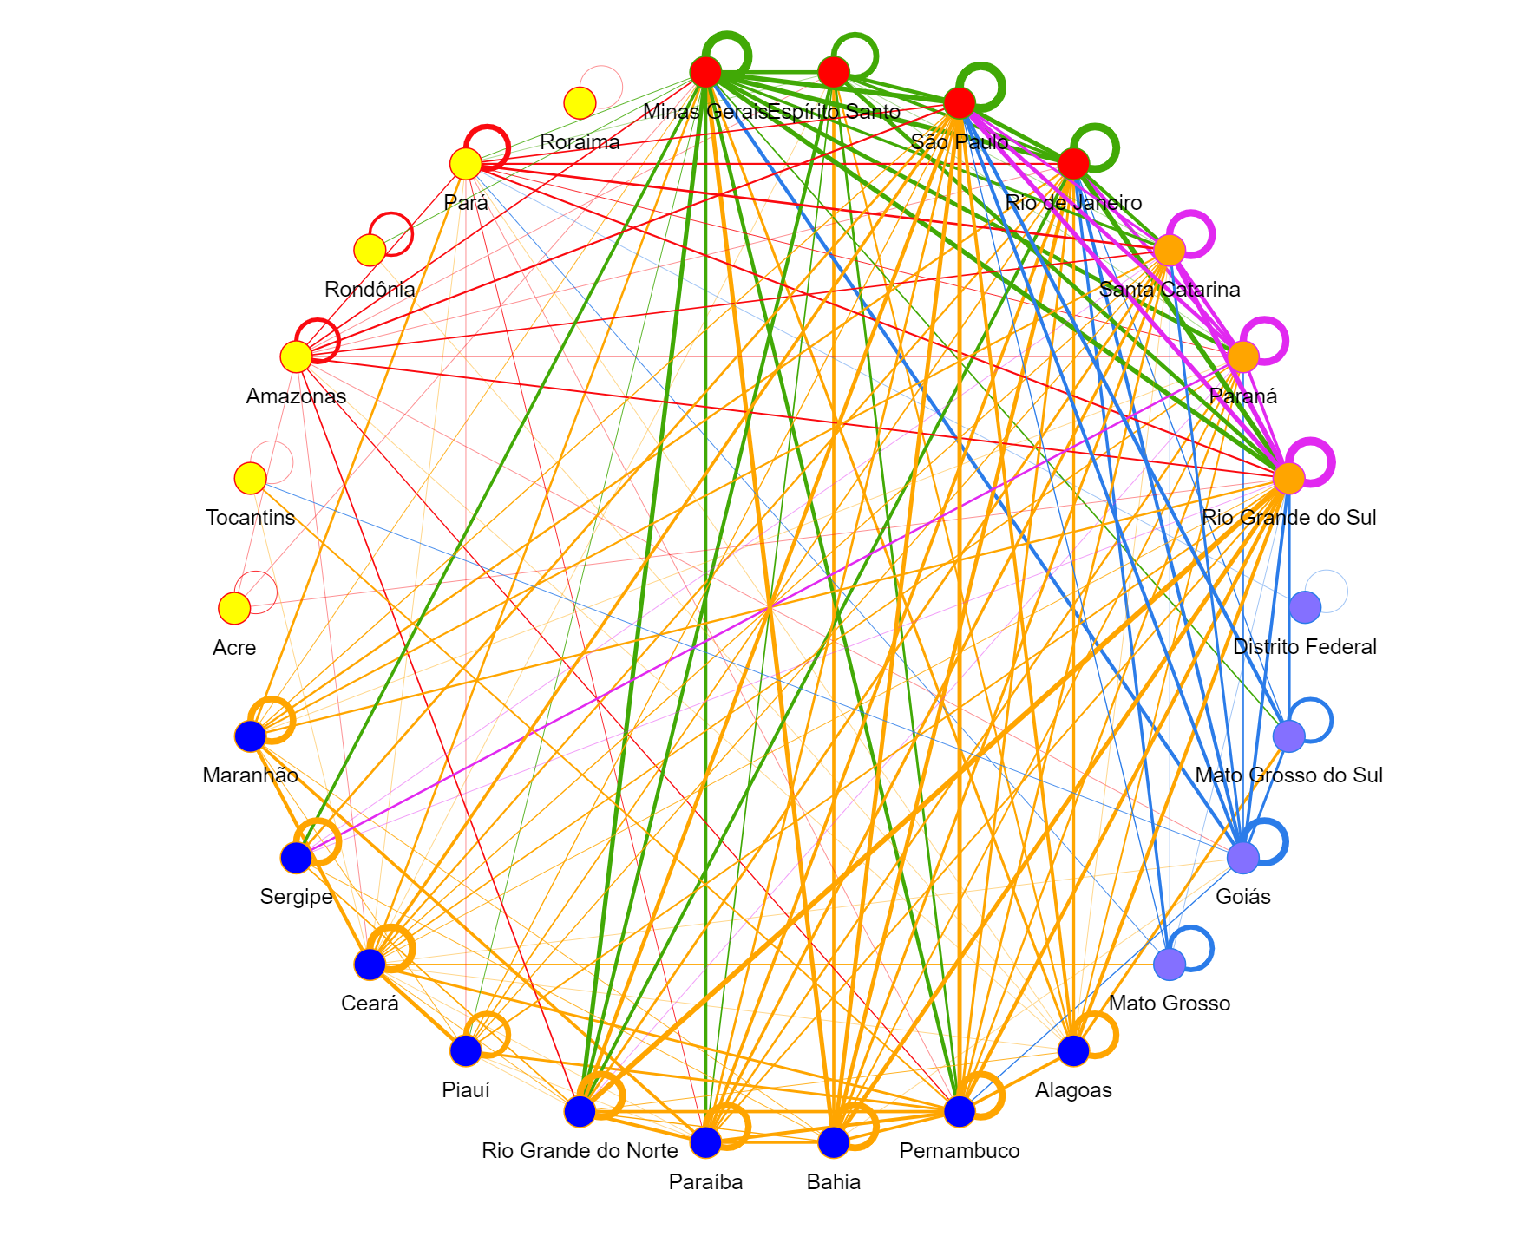
\includegraphics[scale=0.6]{images/rede-2013.pdf}
%\caption{Rede de Coautoria das Universidades Federais do Brasil - 2013}
%\label{Rede de Coautoria - UF BR 2013}
%\end{figure}

%\begin{figure}[H]
%\centering
%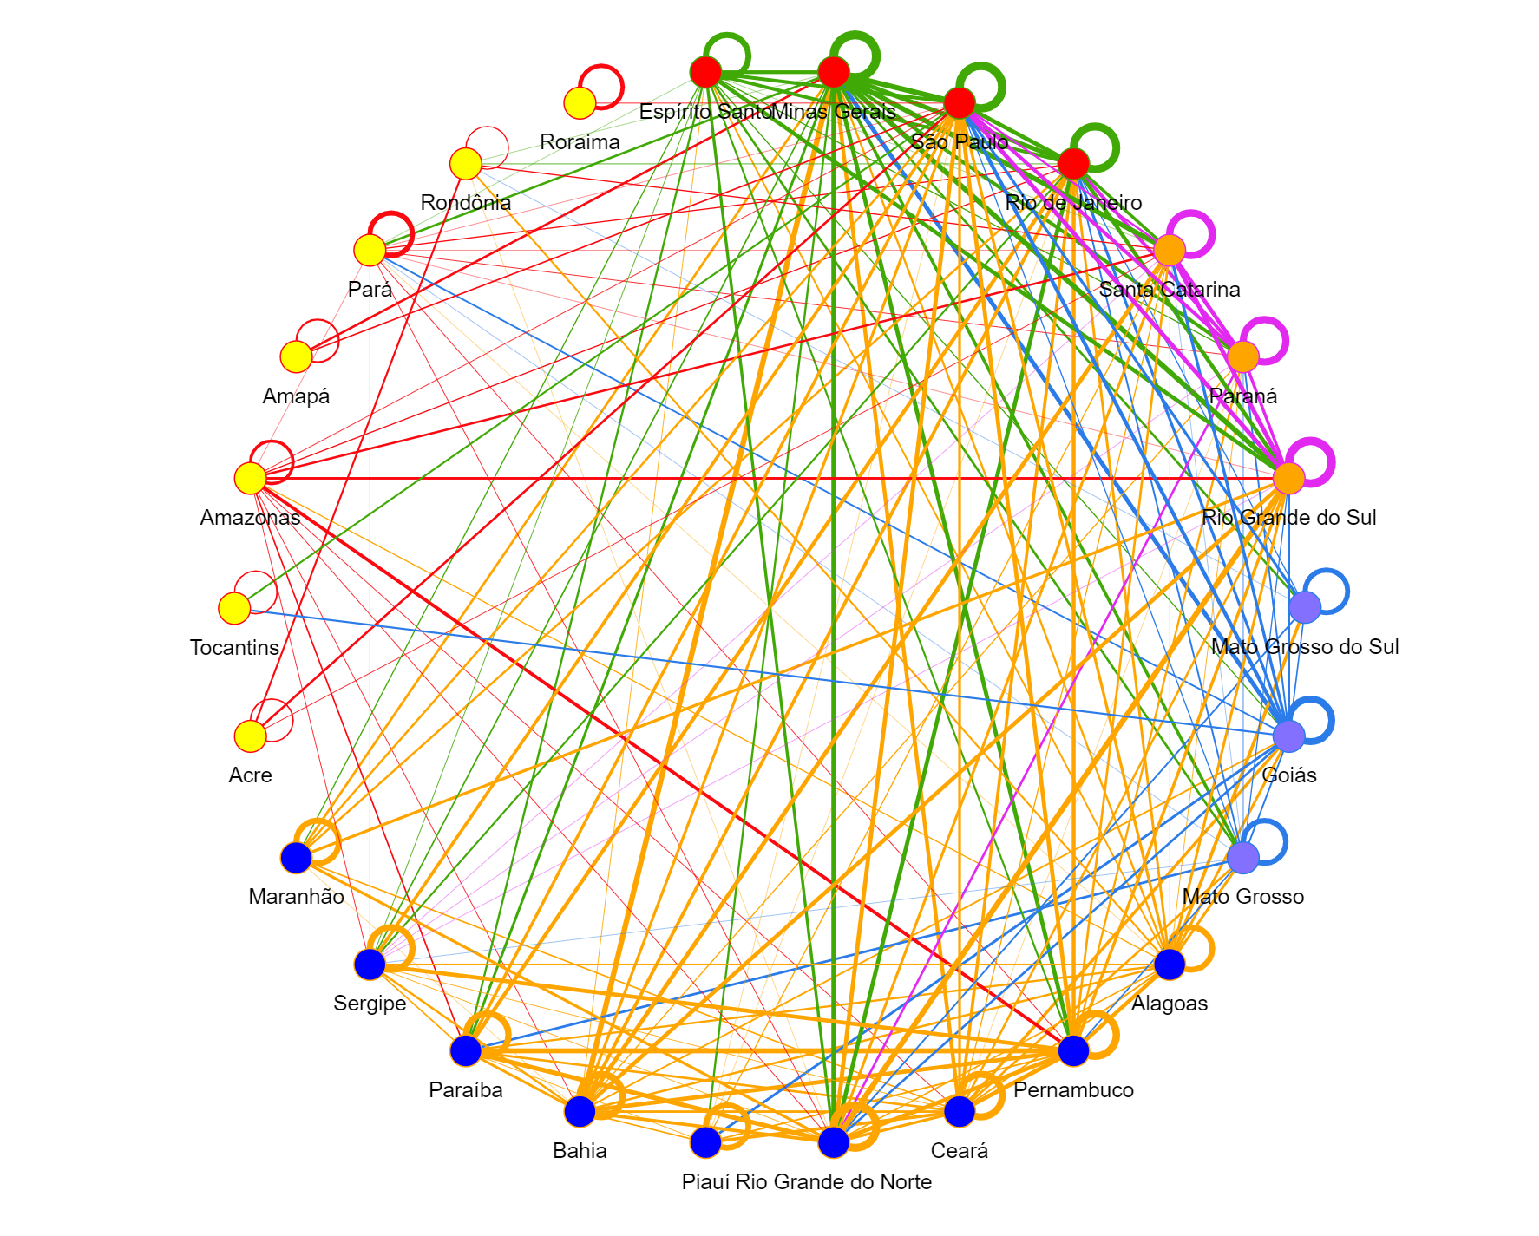
\includegraphics[scale=0.6]{images/rede-2017.pdf}
%\caption{Rede de Coautoria das Universidades Federais do Brasil - 2007}
%\label{Rede de Coautoria - UF BR 2017}
%\end{figure}

<<<<<<< HEAD
=======
\section{Região Centro-Oeste}
>>>>>>> cd3e754ceb877b541239e23f642a5c9aa00f96c6


\begin{figure}[H]
\begin{tabular}{ccc}
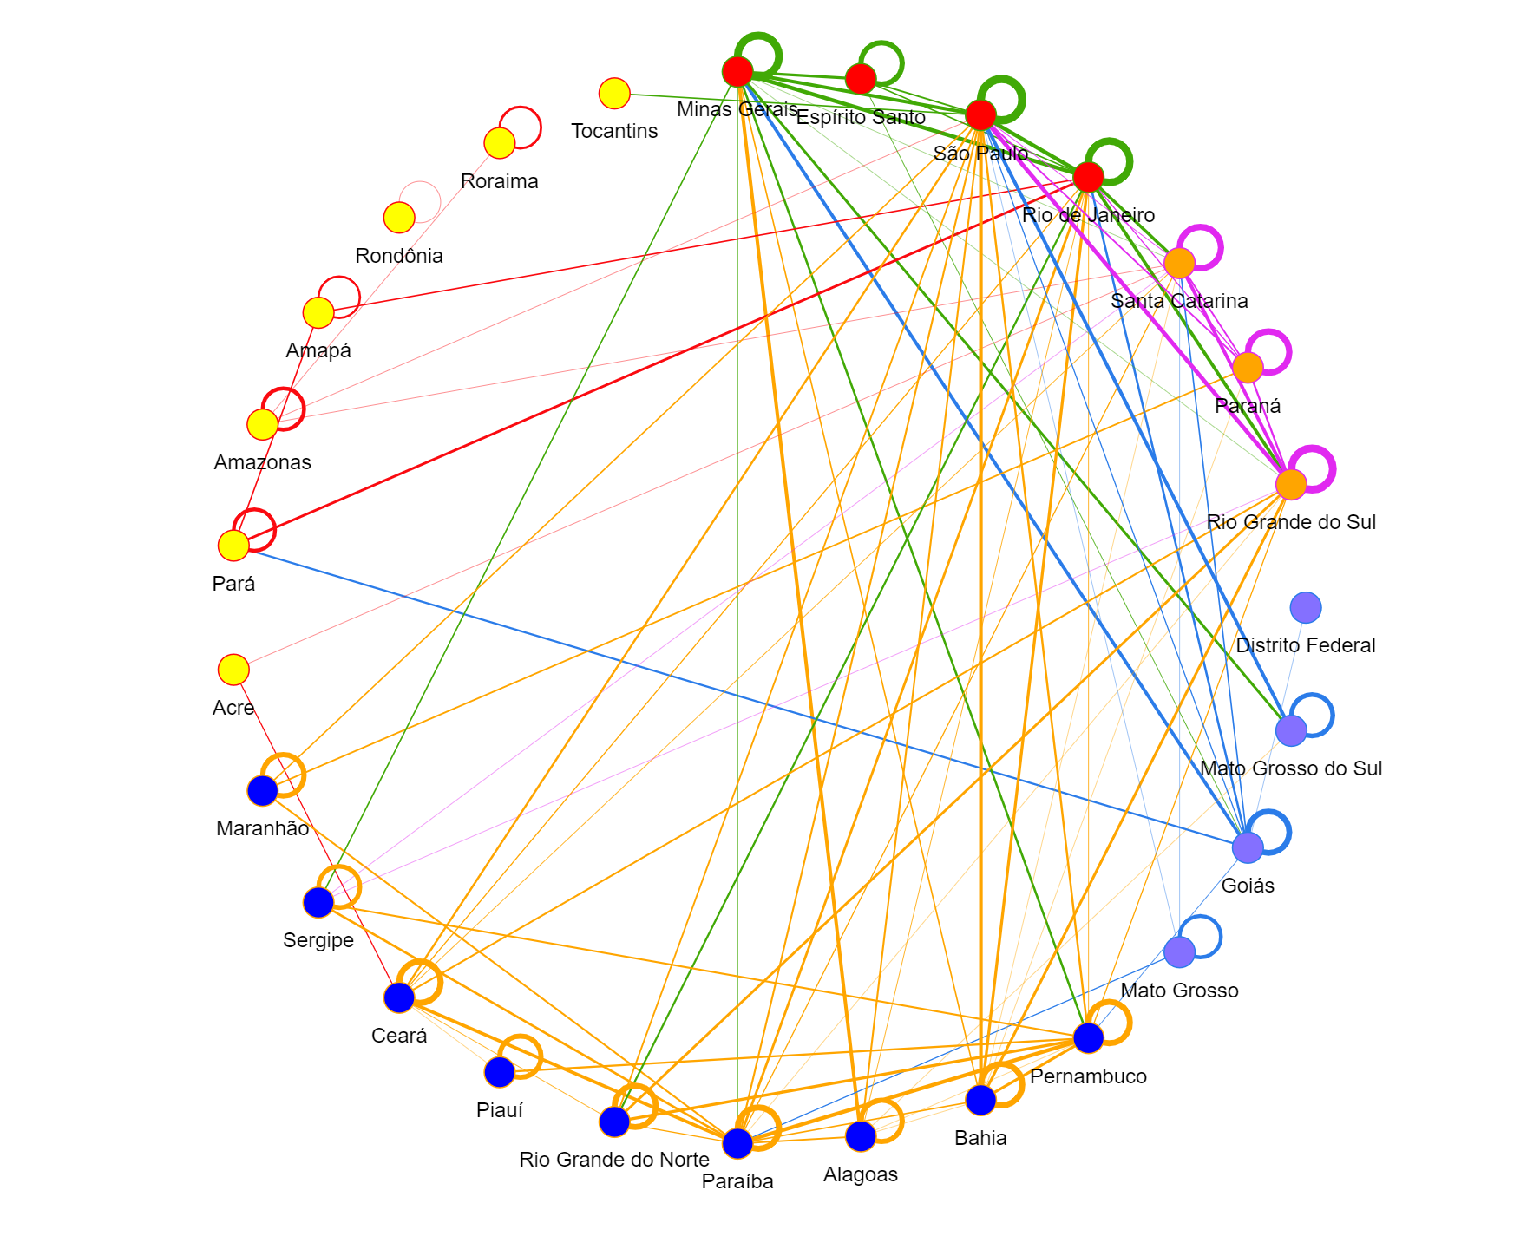
\includegraphics[width=0.35\textwidth]{images/rede-2008.pdf} &   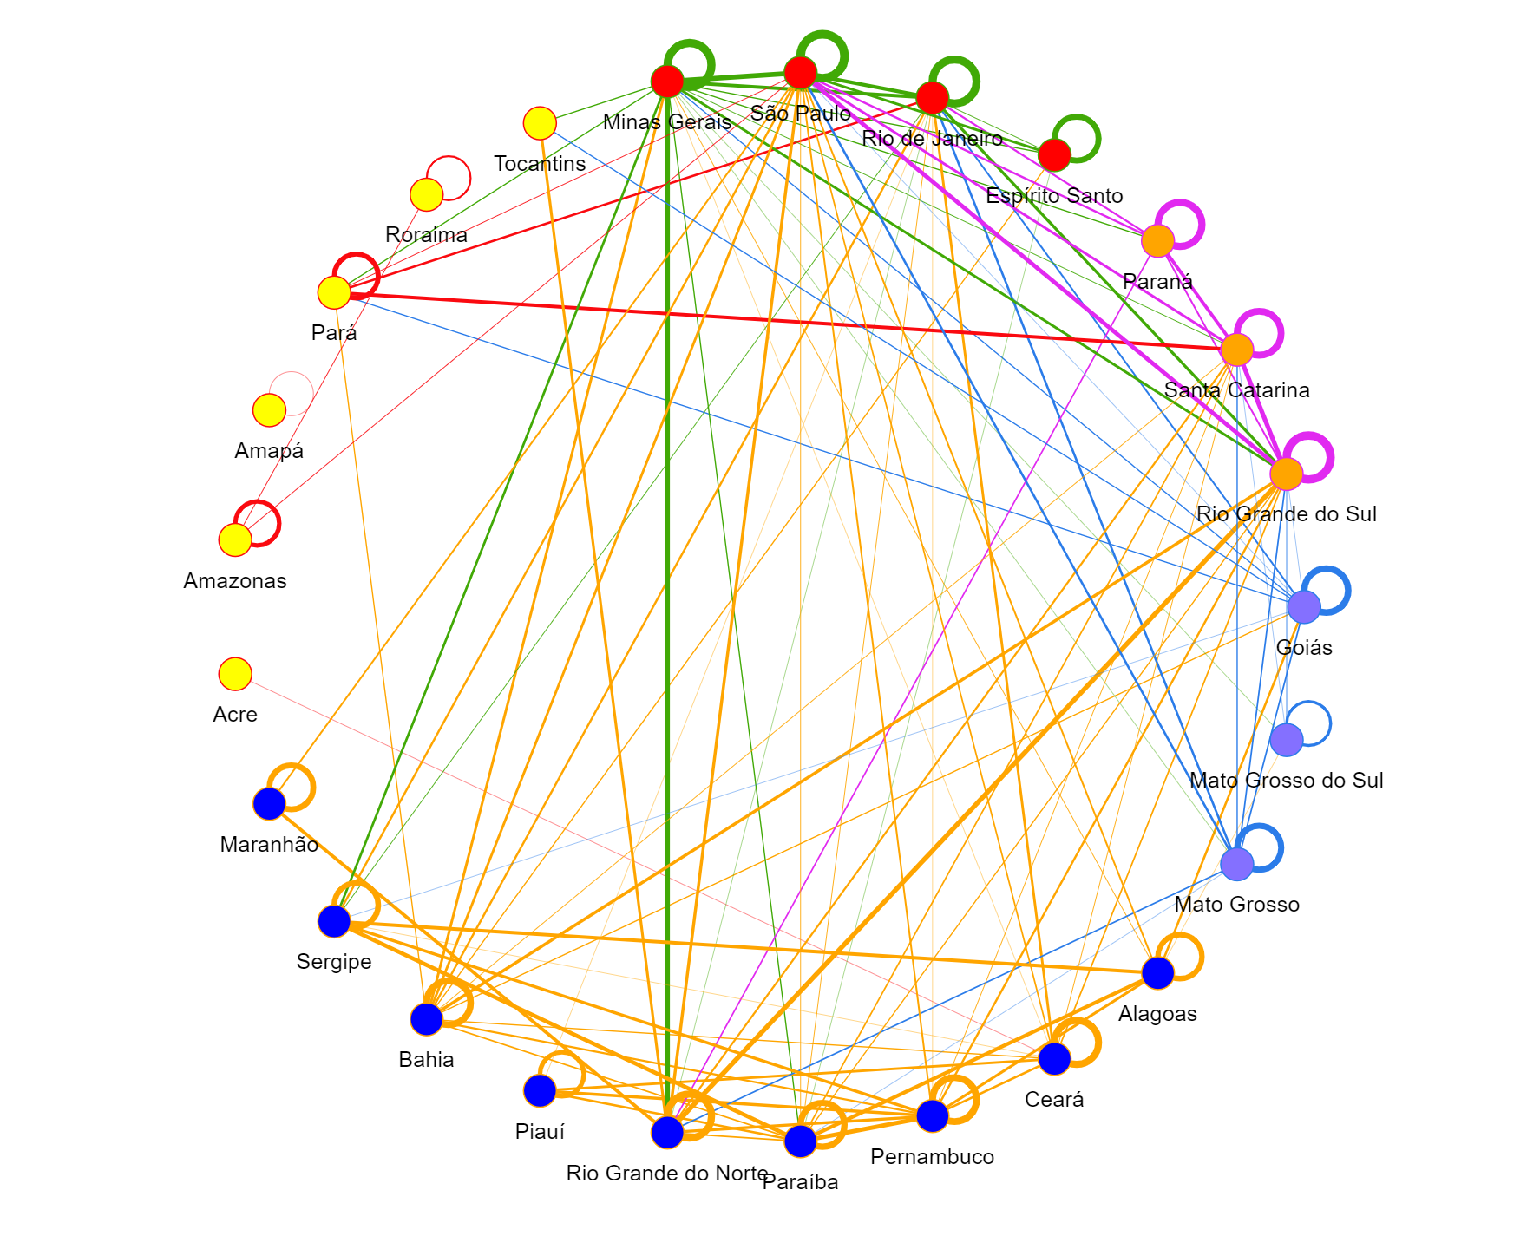
\includegraphics[width=0.35\textwidth]{images/rede-2009.pdf} &
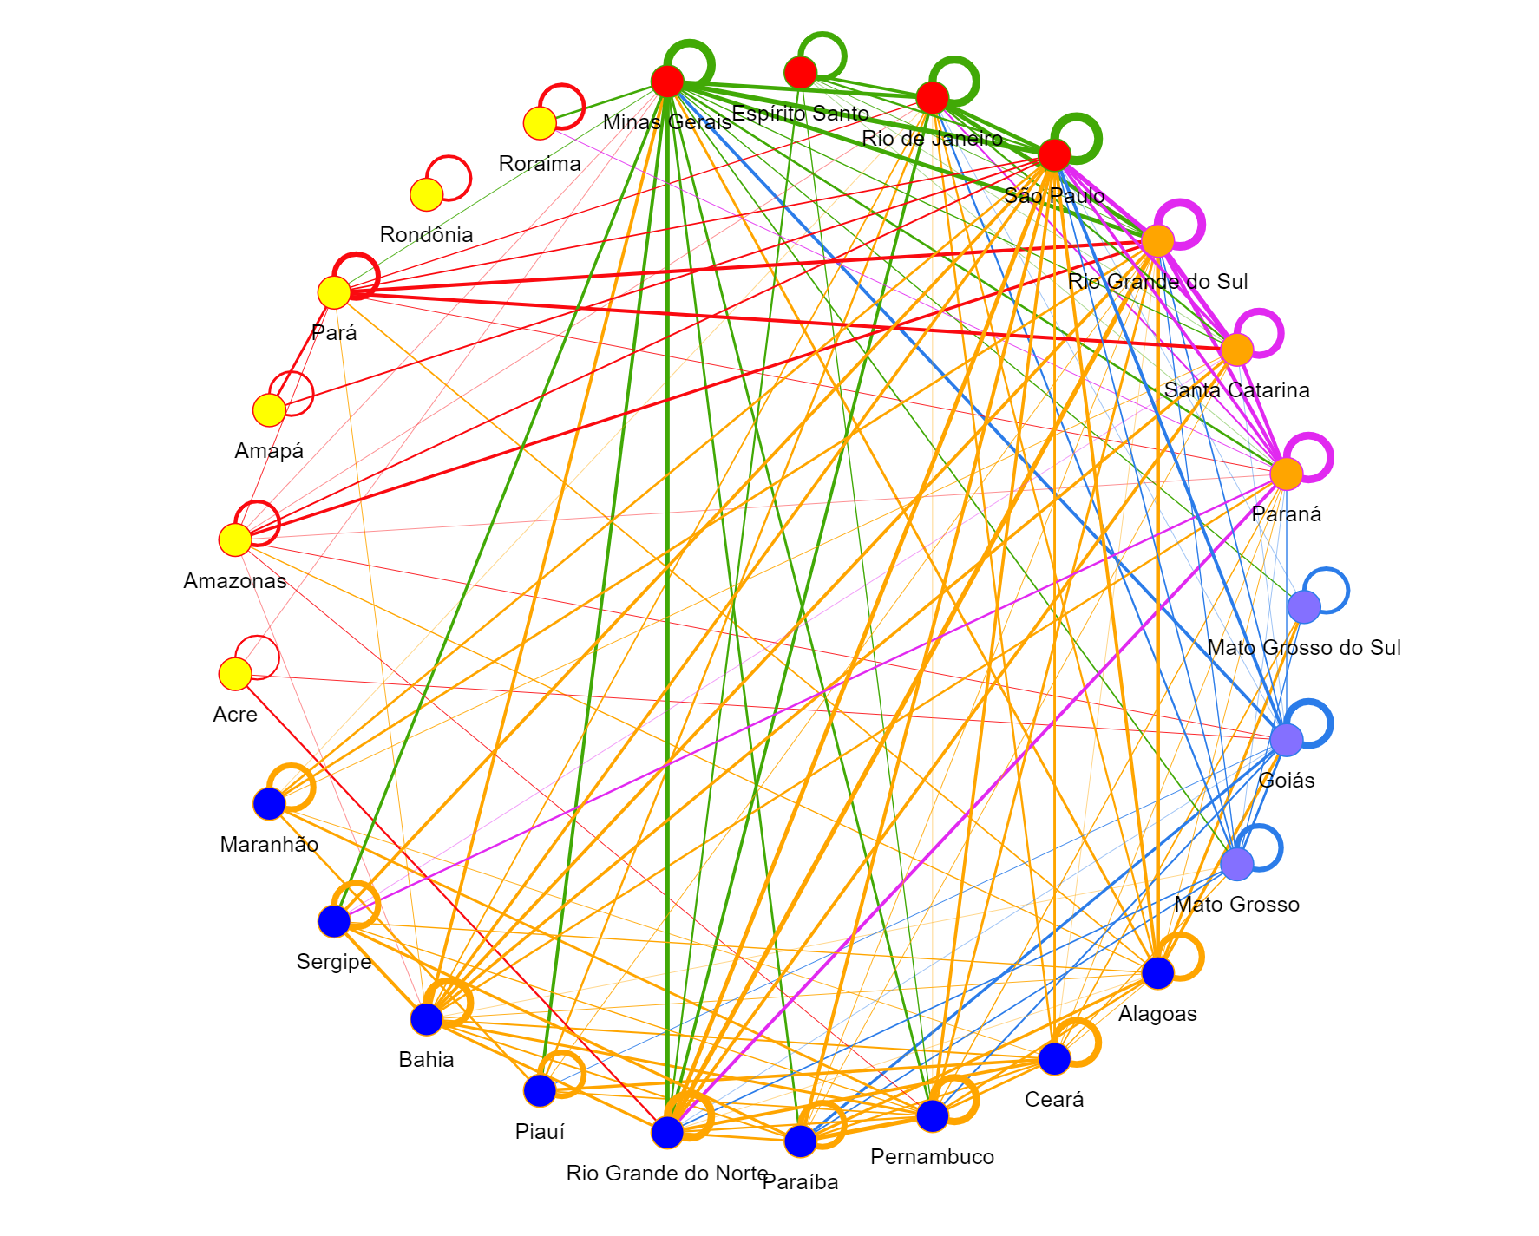
\includegraphics[width=0.35\textwidth]{images/rede-2010.pdf}\\
2008 & 2009 & 2010\\[6pt] 
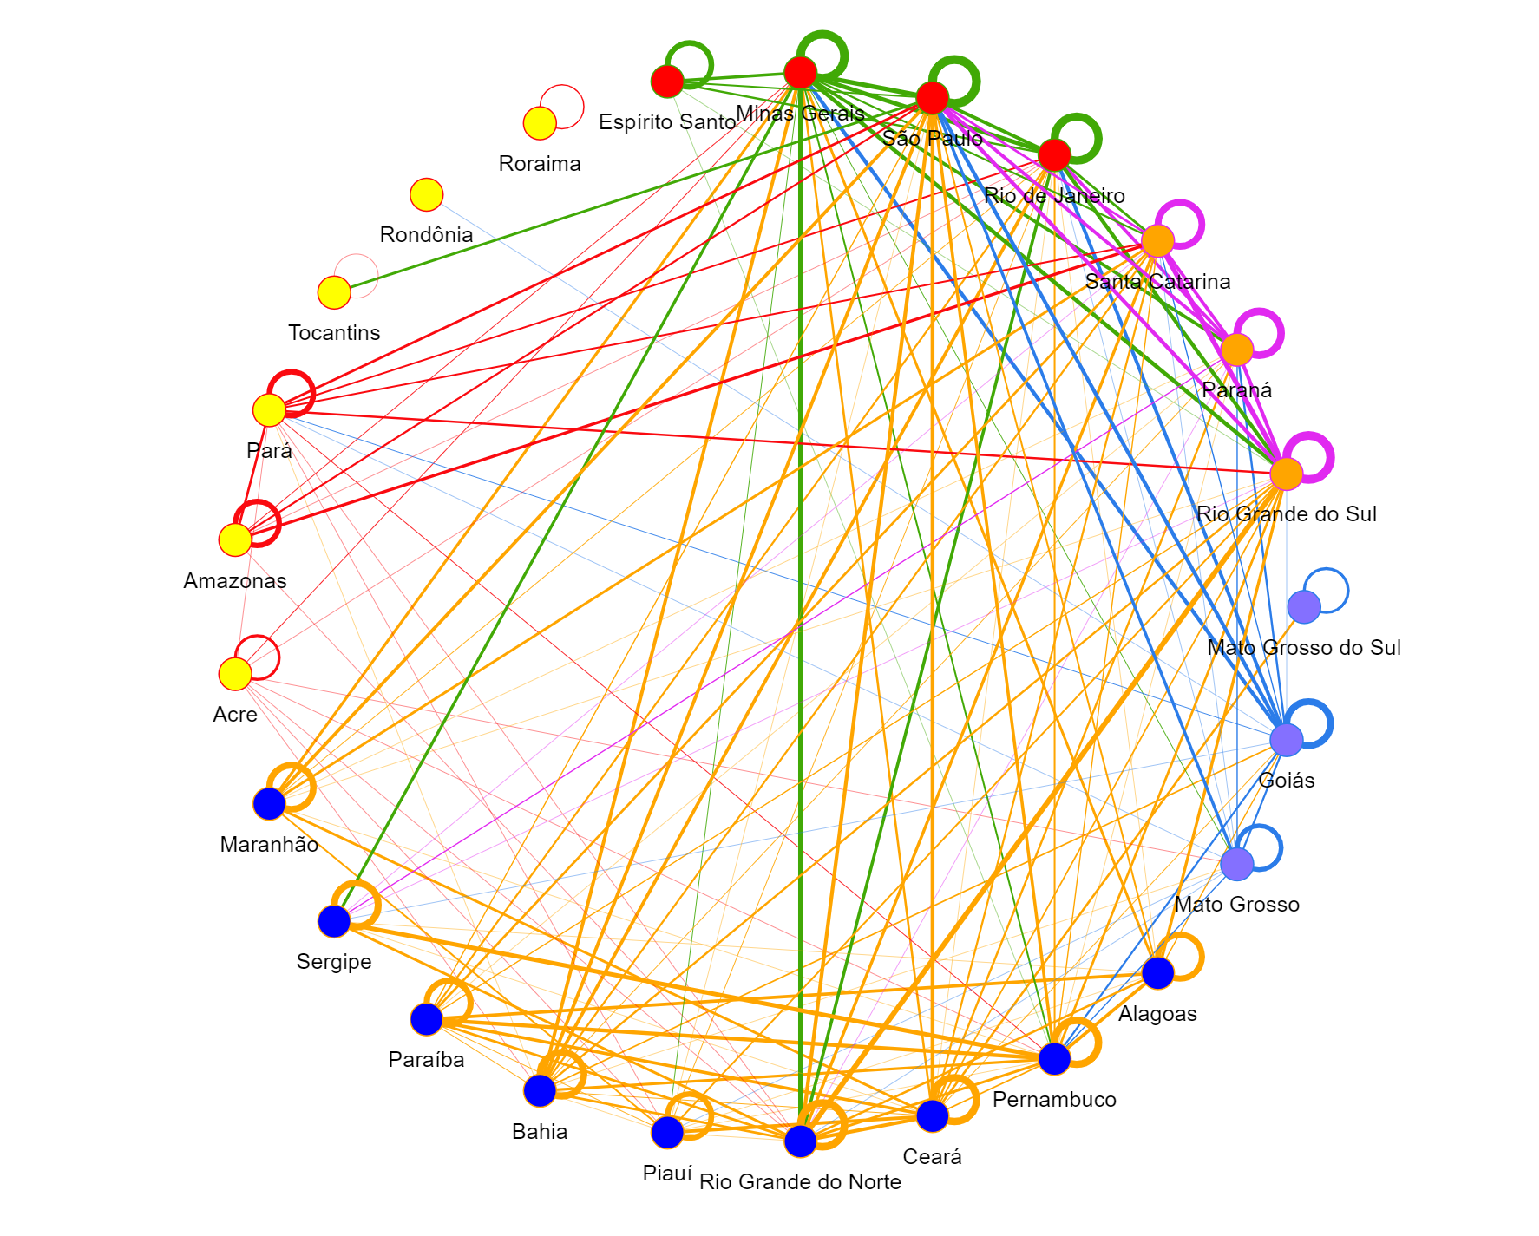
\includegraphics[width=0.35\textwidth]{images/rede-2011.pdf} &
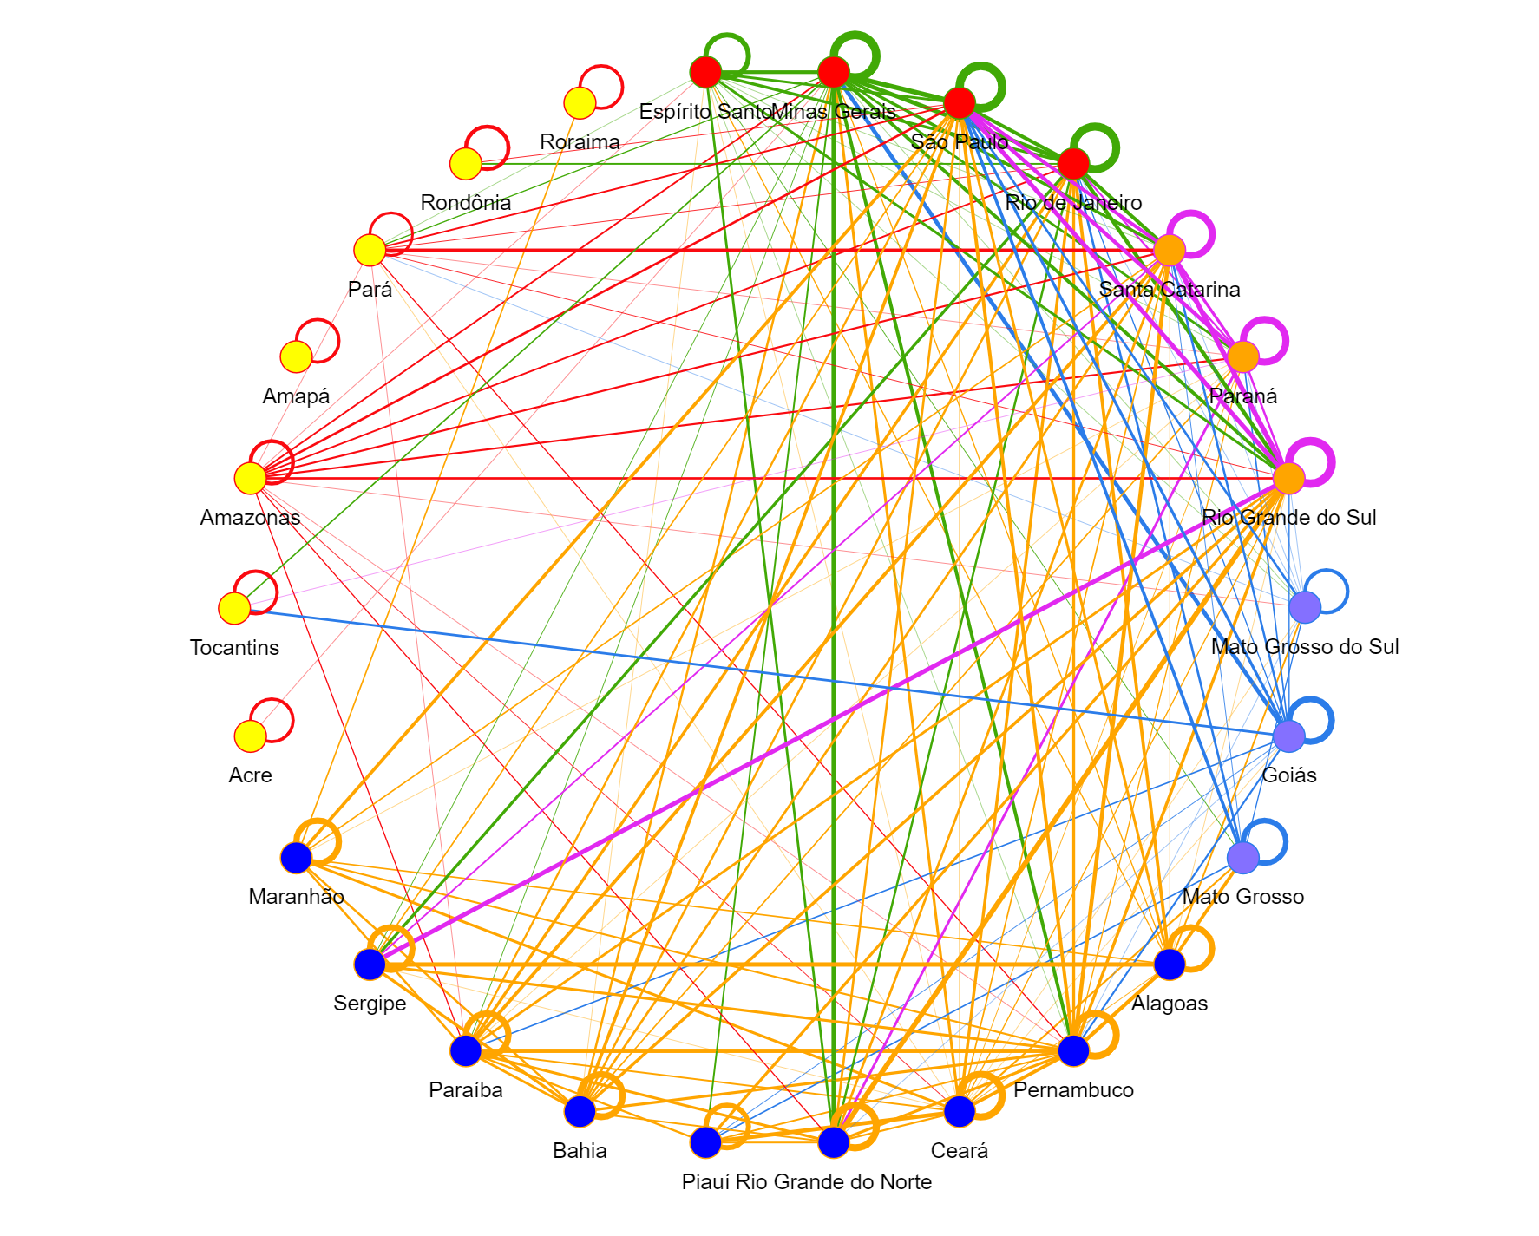
\includegraphics[width=0.35\textwidth]{images/rede-2012.pdf} &   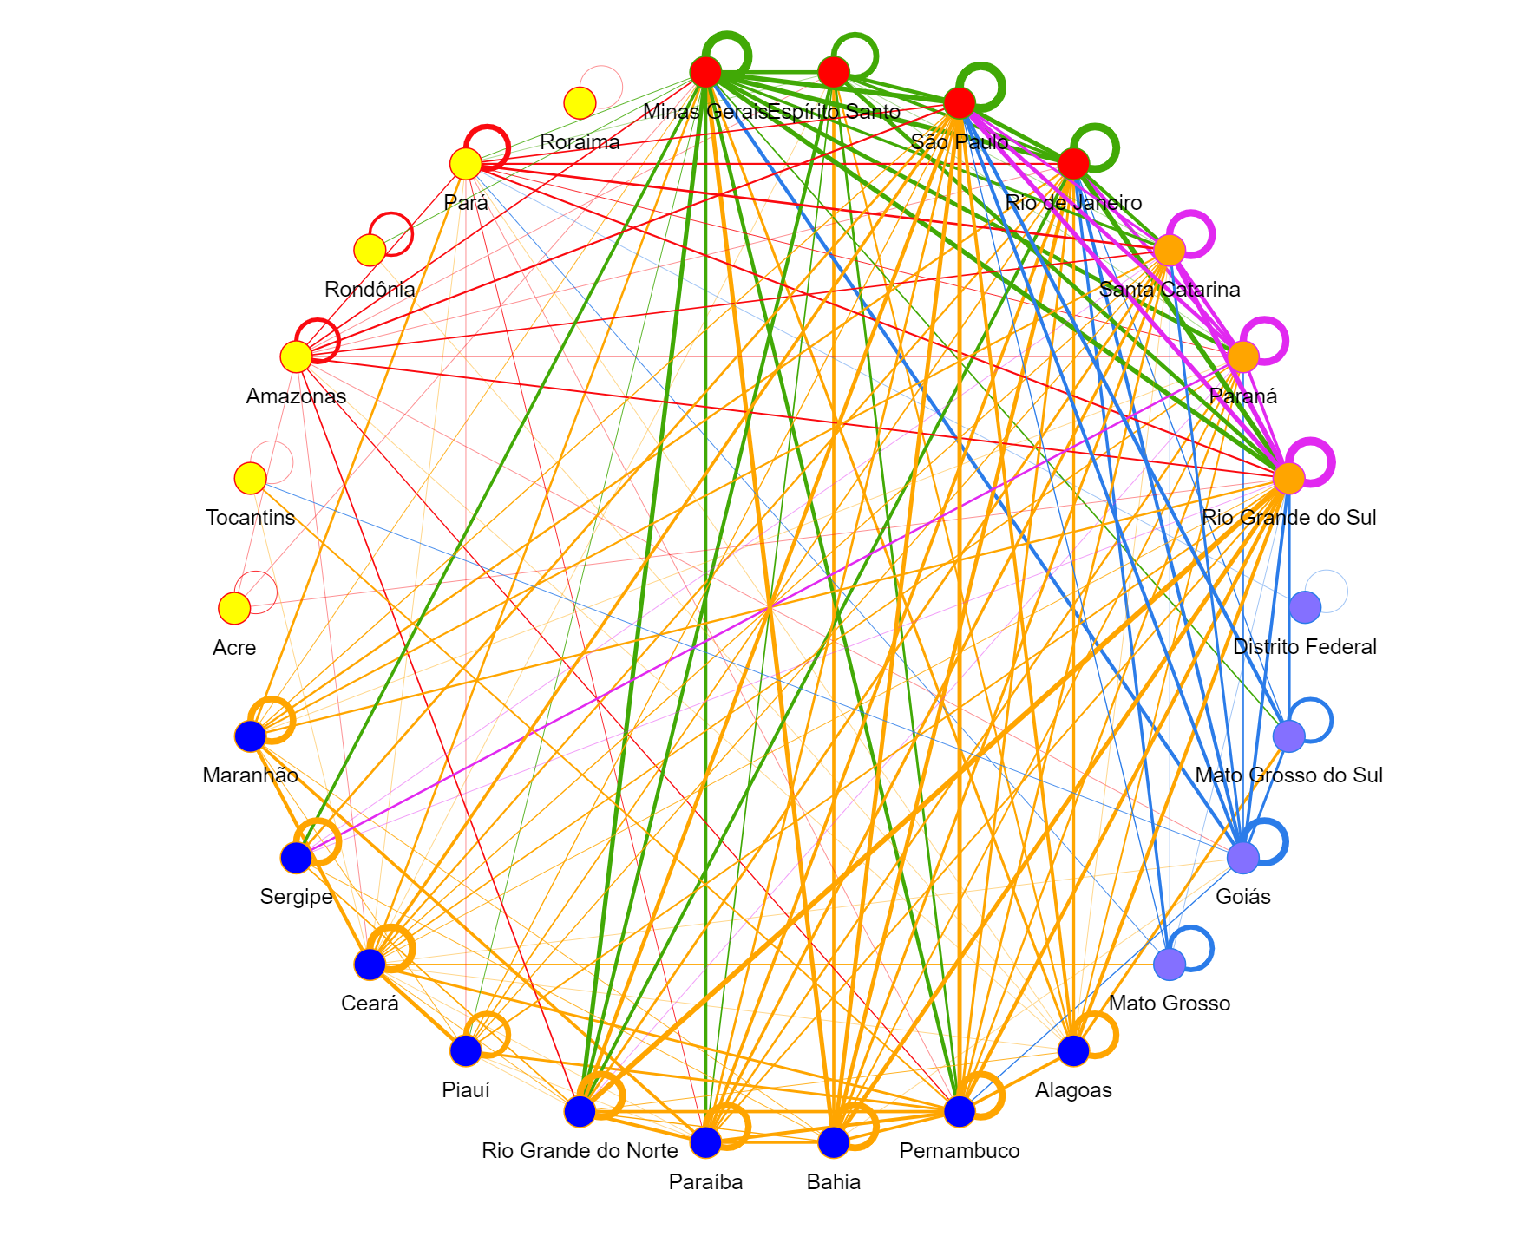
\includegraphics[width=0.35\textwidth]{images/rede-2013.pdf} \\
2011 & 2012 & 2013\\[6pt]
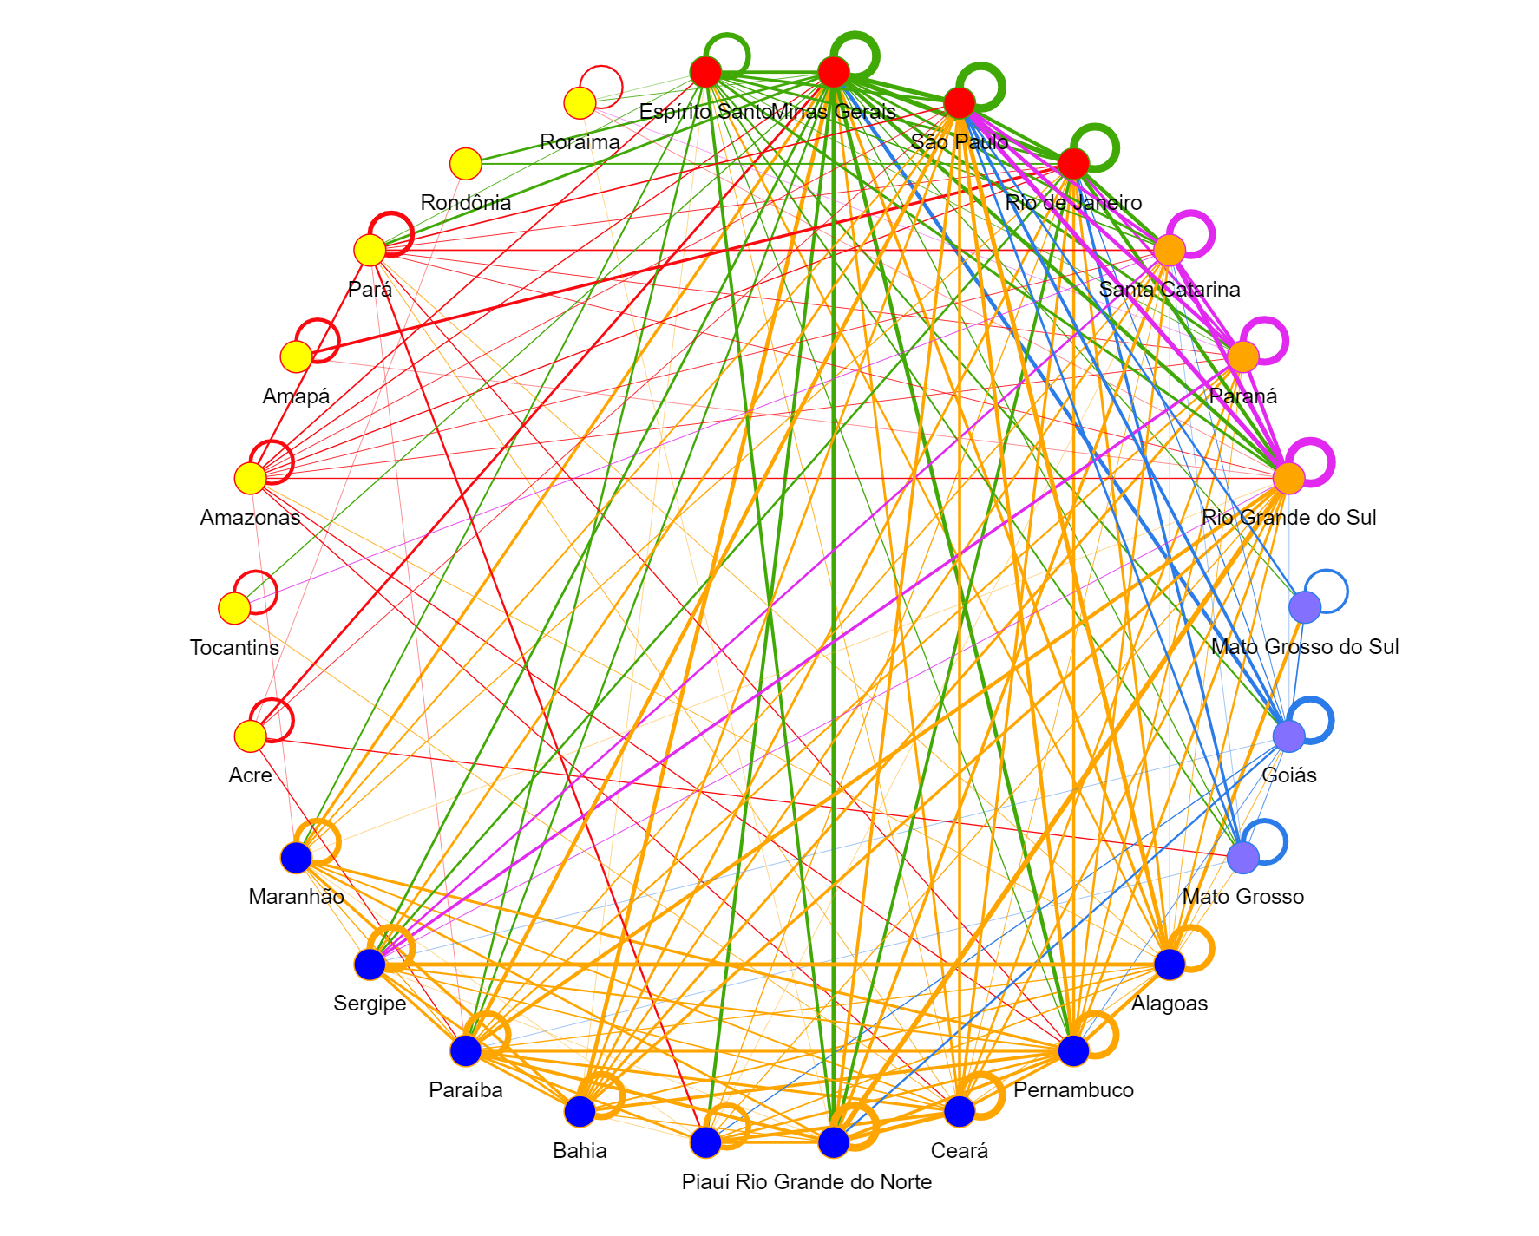
\includegraphics[width=0.35\textwidth]{images/rede-2014.pdf} &
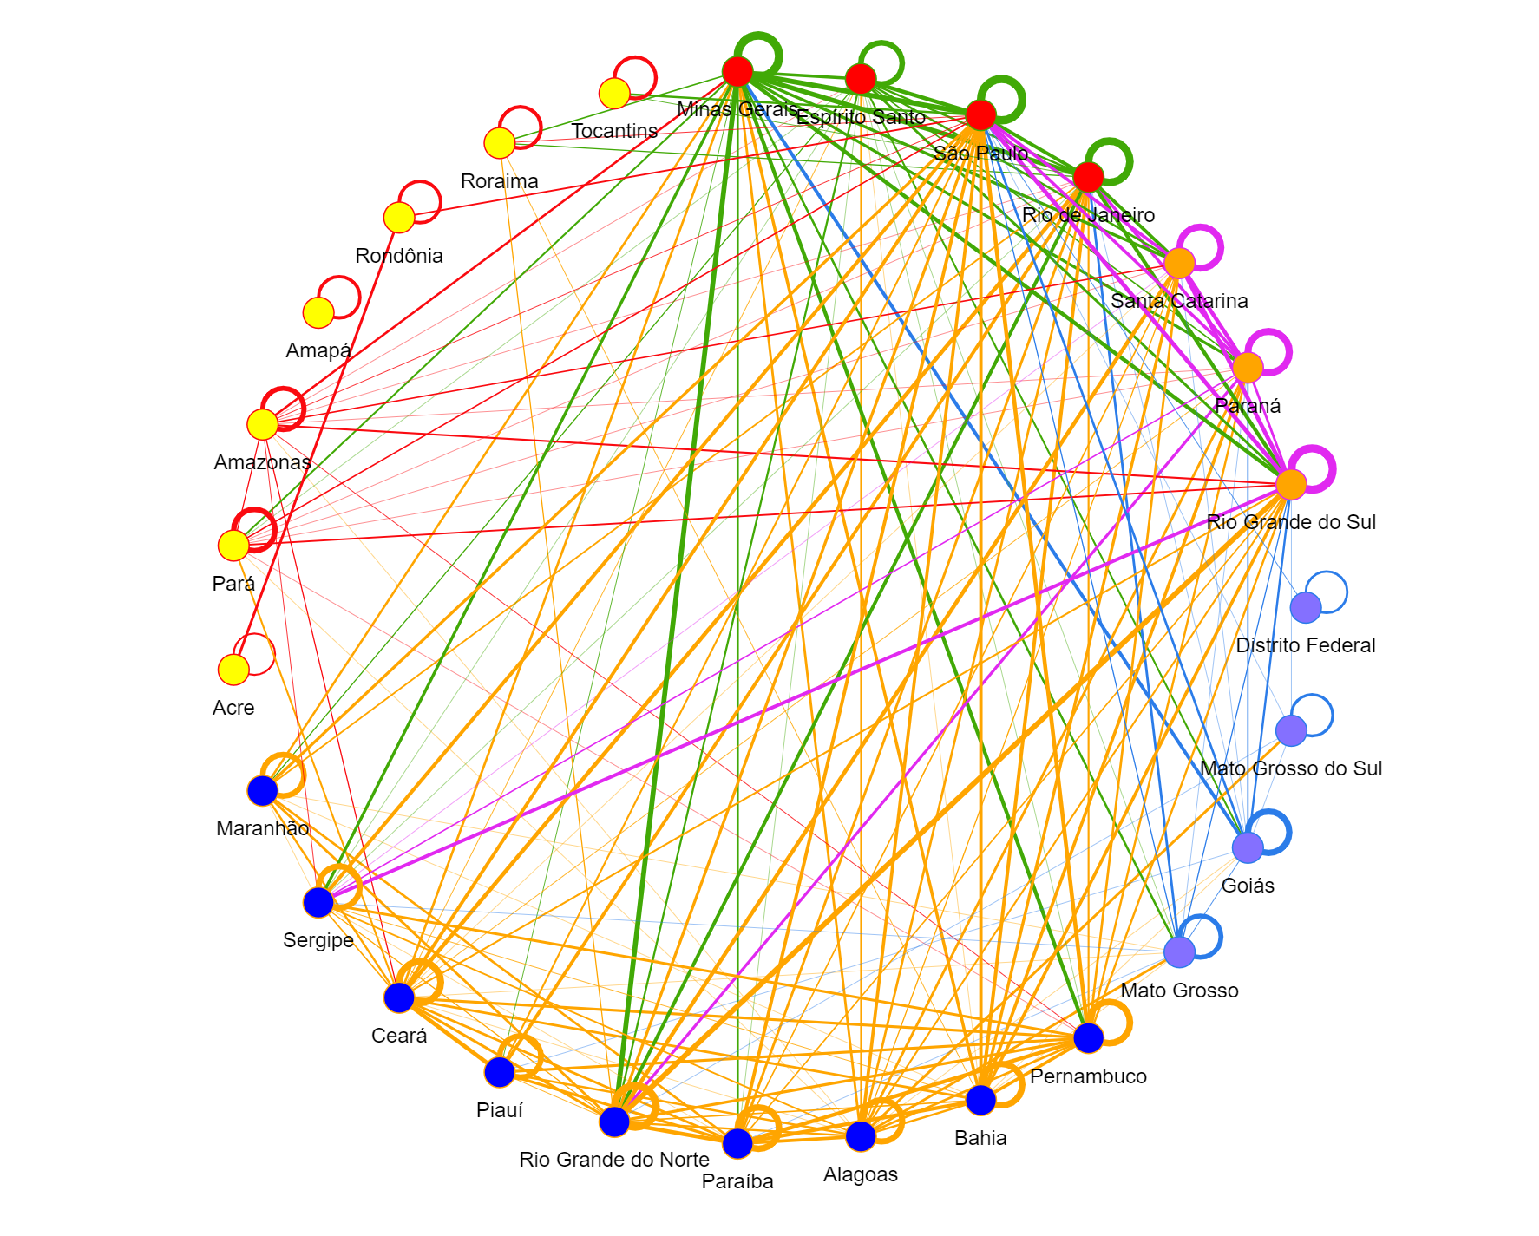
\includegraphics[width=0.35\textwidth]{images/rede-2015.pdf} &
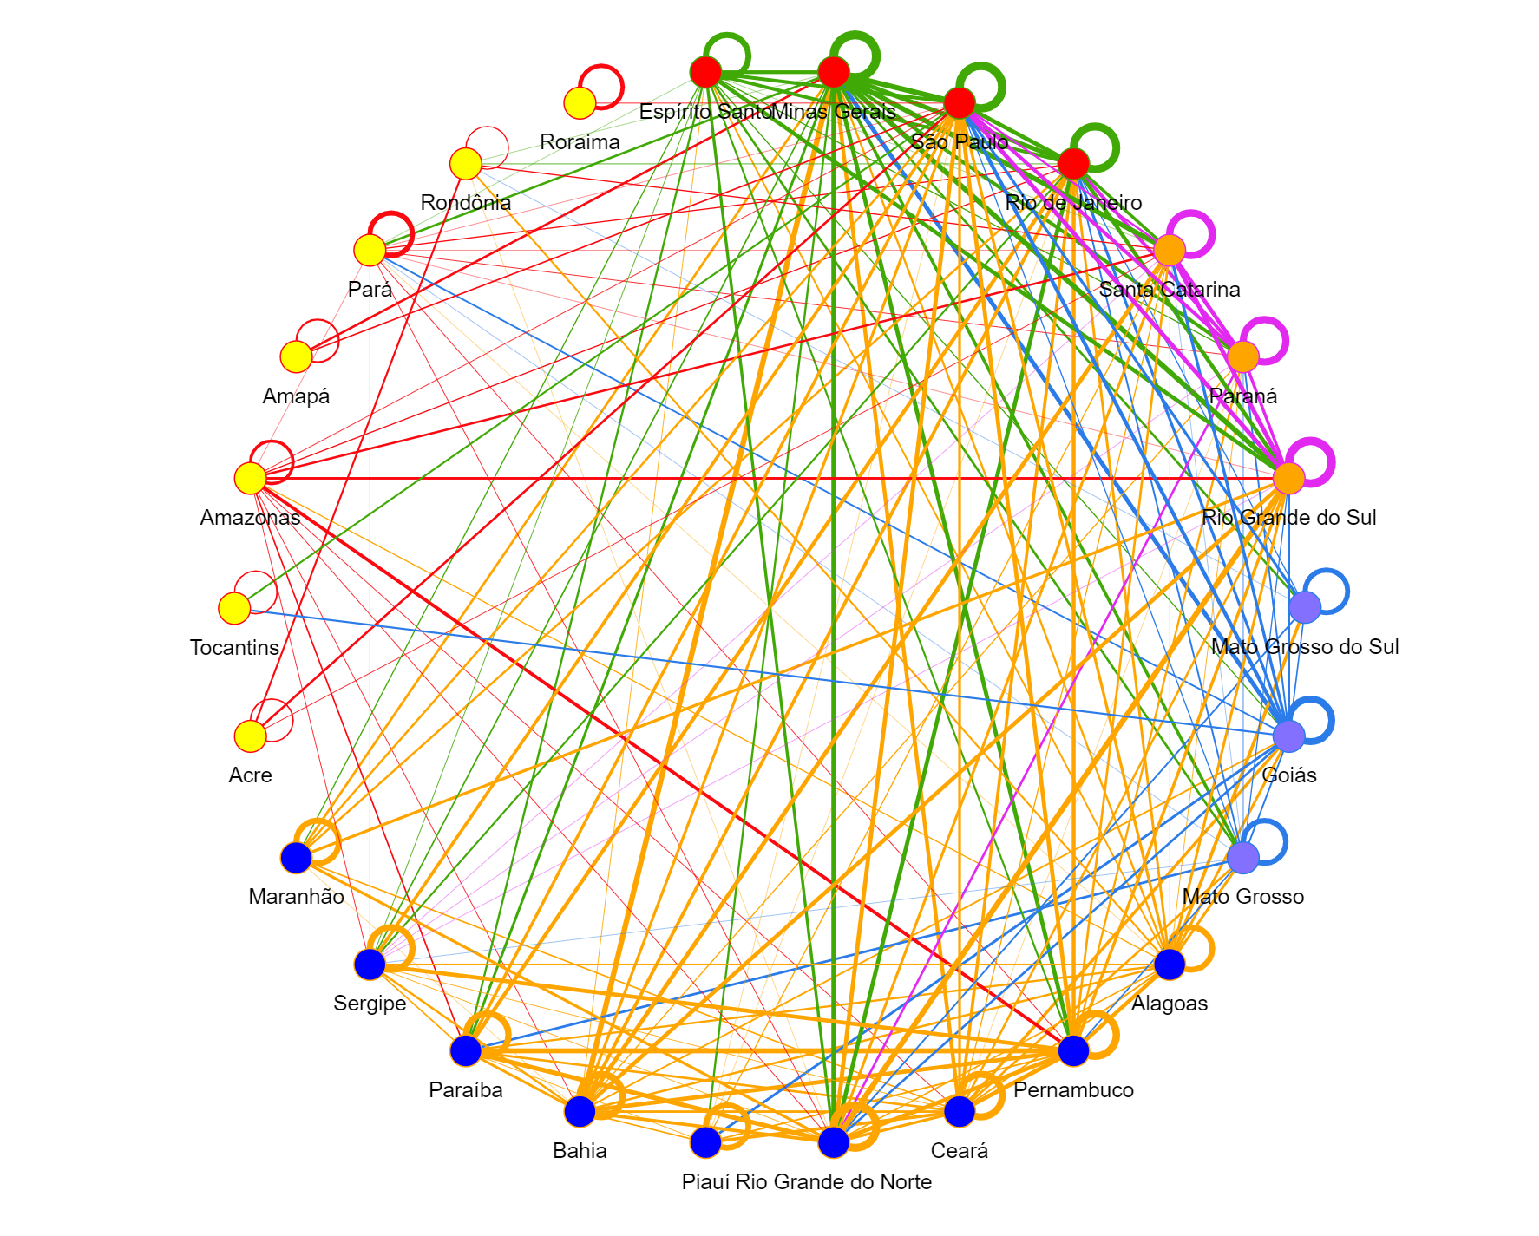
\includegraphics[width=0.35\textwidth]{images/rede-2016.pdf} \\
2014 & 2015 & 2016\\[6pt]  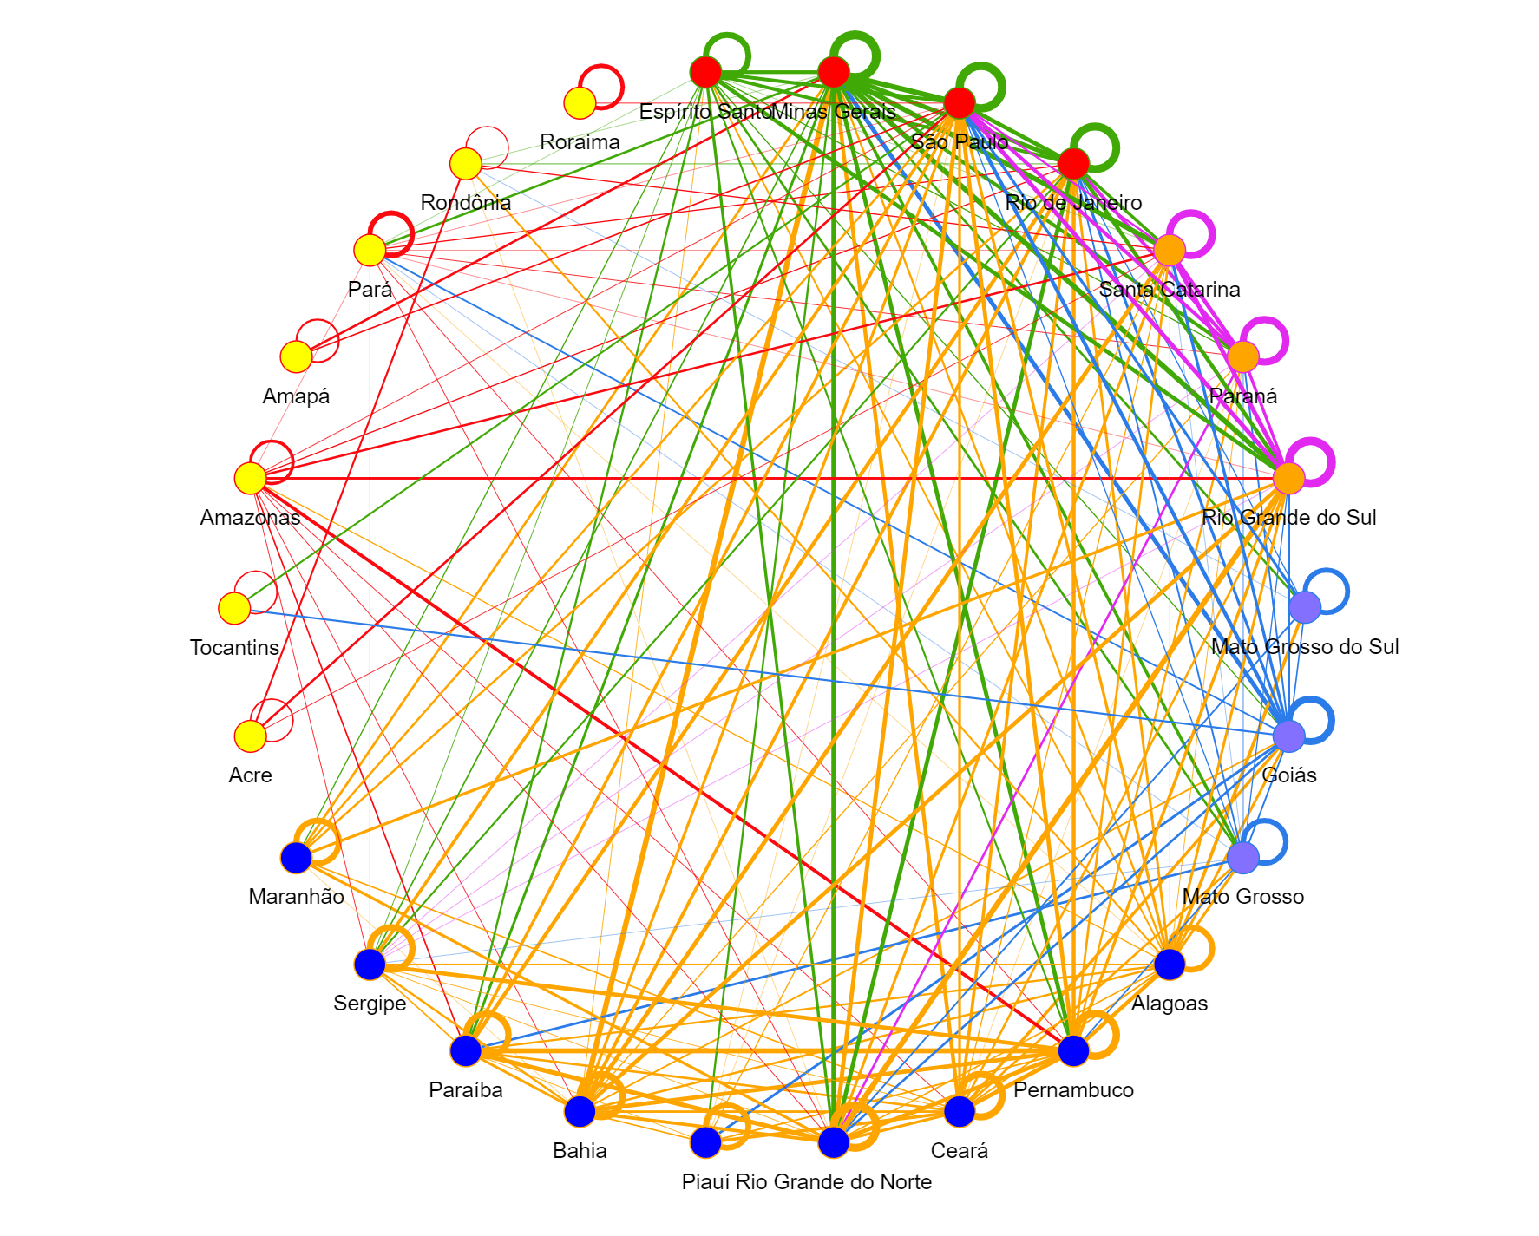
\includegraphics[width=0.35\textwidth]{images/rede-2017.pdf} & & \\
2017 & & \\
\end{tabular}
\caption{Redes de Coautoria Universidades Federal do Brasil}
\end{figure}





\subsubsection{Rede de Coautoria Brasil - Vértice Focal Alagoas}

A seguir são apresentadas as redes de coautoria utilizando o vértice focal Alagoas, e então observando as conexões realizadas com os demais vértices da rede (UF). Visualmente é possível notar o crescimento pelo número de novas conexões.


\begin{figure}[H]
\begin{tabular}{ccc}
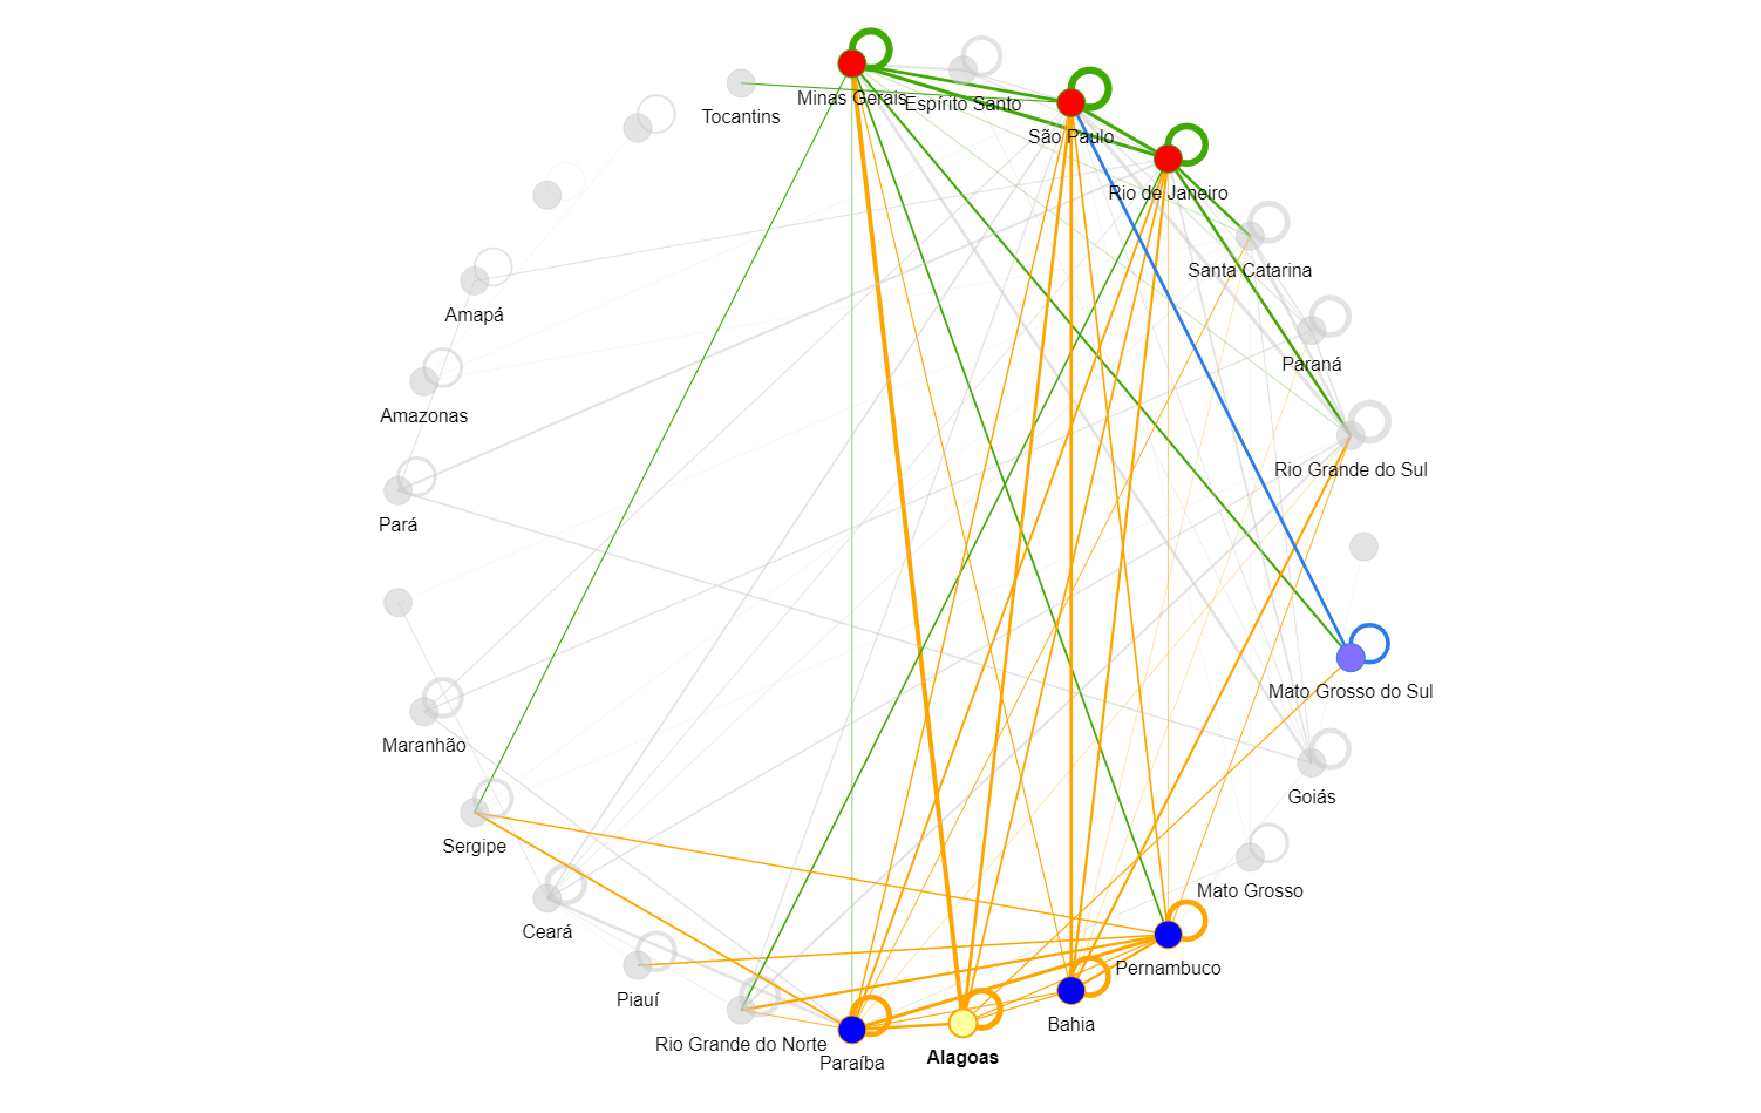
\includegraphics[width=0.38\textwidth]{images/rede-al-2008.pdf} &   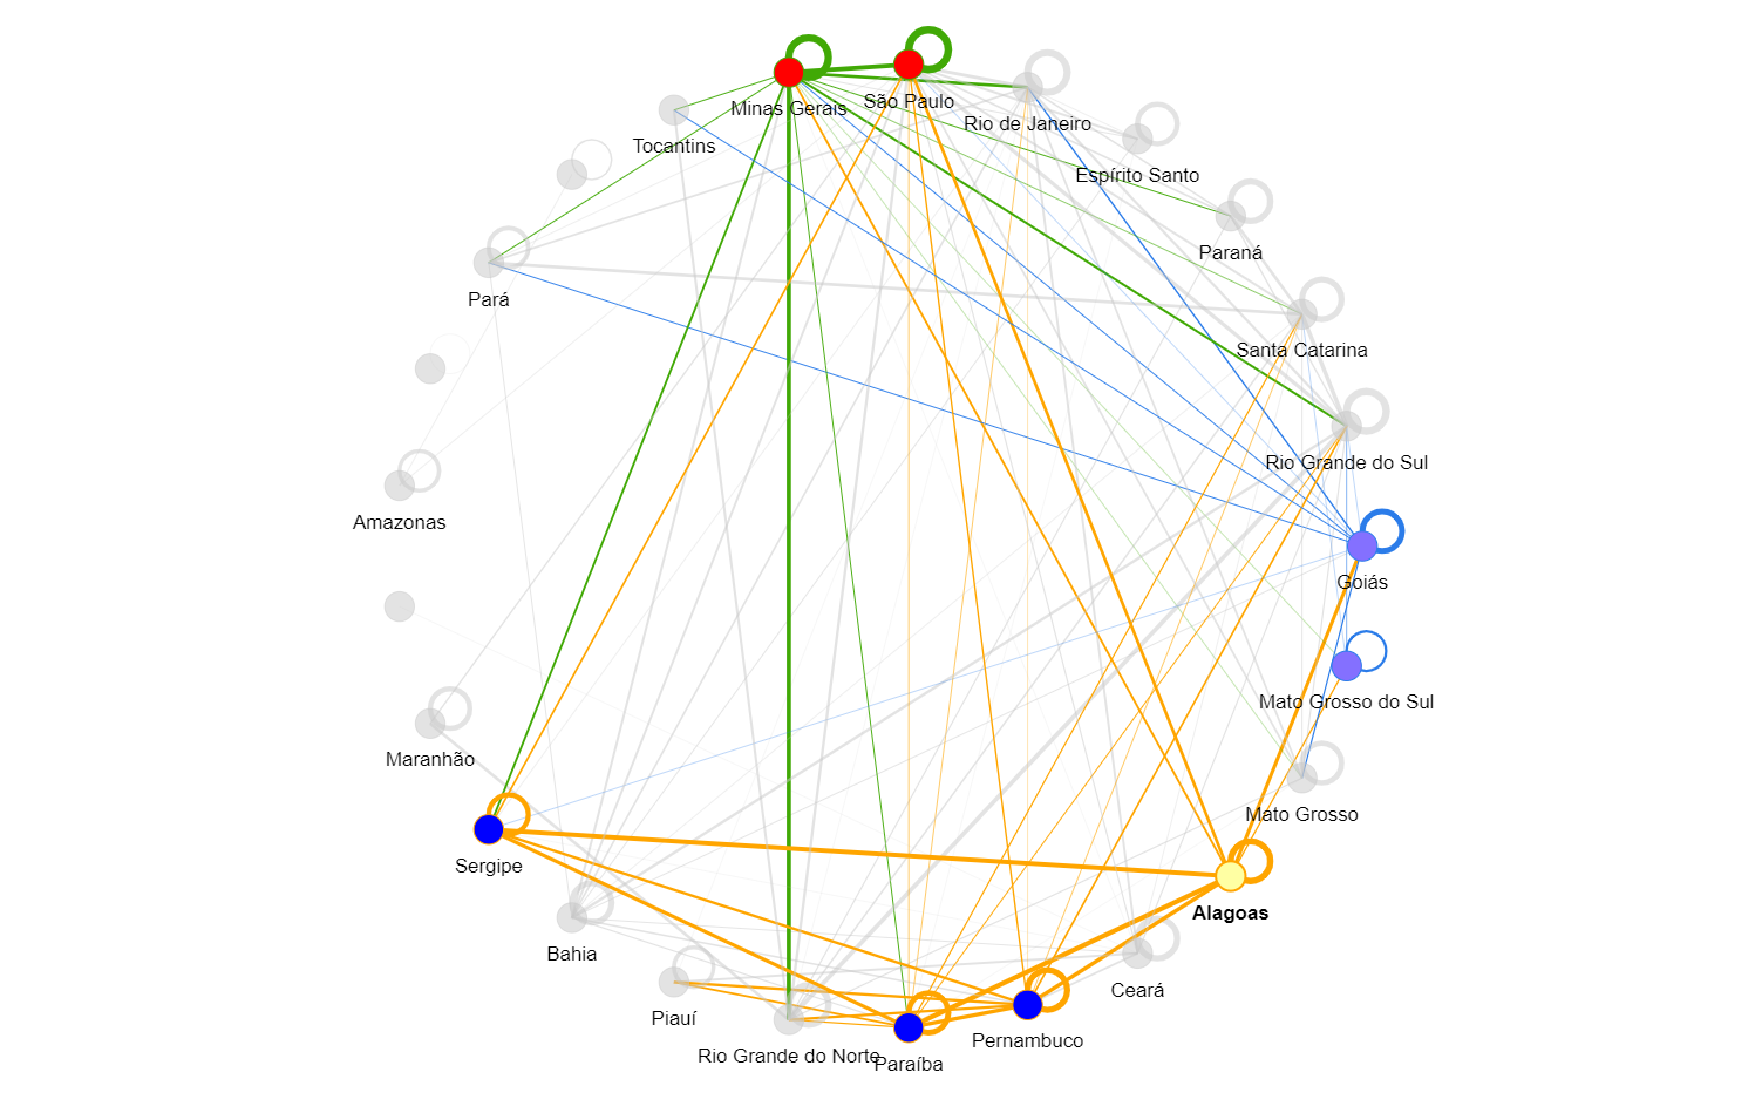
\includegraphics[width=0.38\textwidth]{images/rede-al-2009.pdf} &
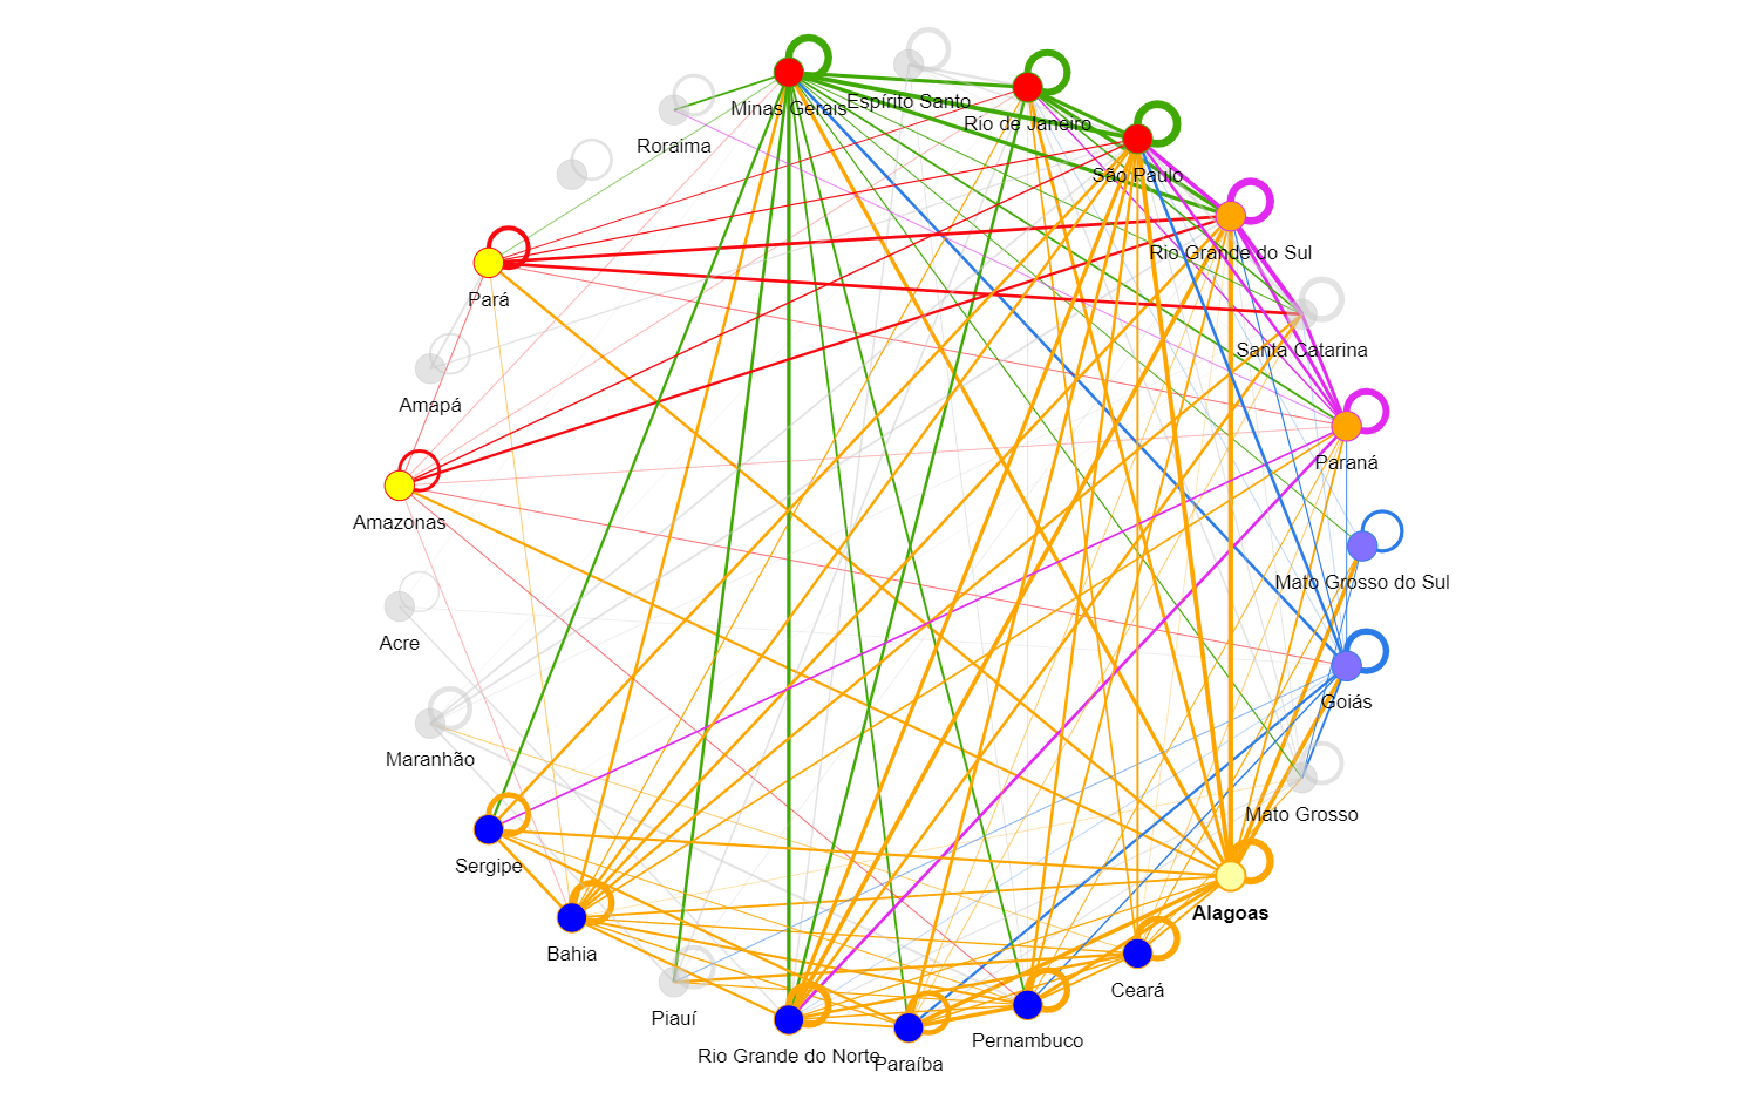
\includegraphics[width=0.38\textwidth]{images/rede-al-2010.pdf}\\
2008 & 2009 & 2010\\[6pt] 
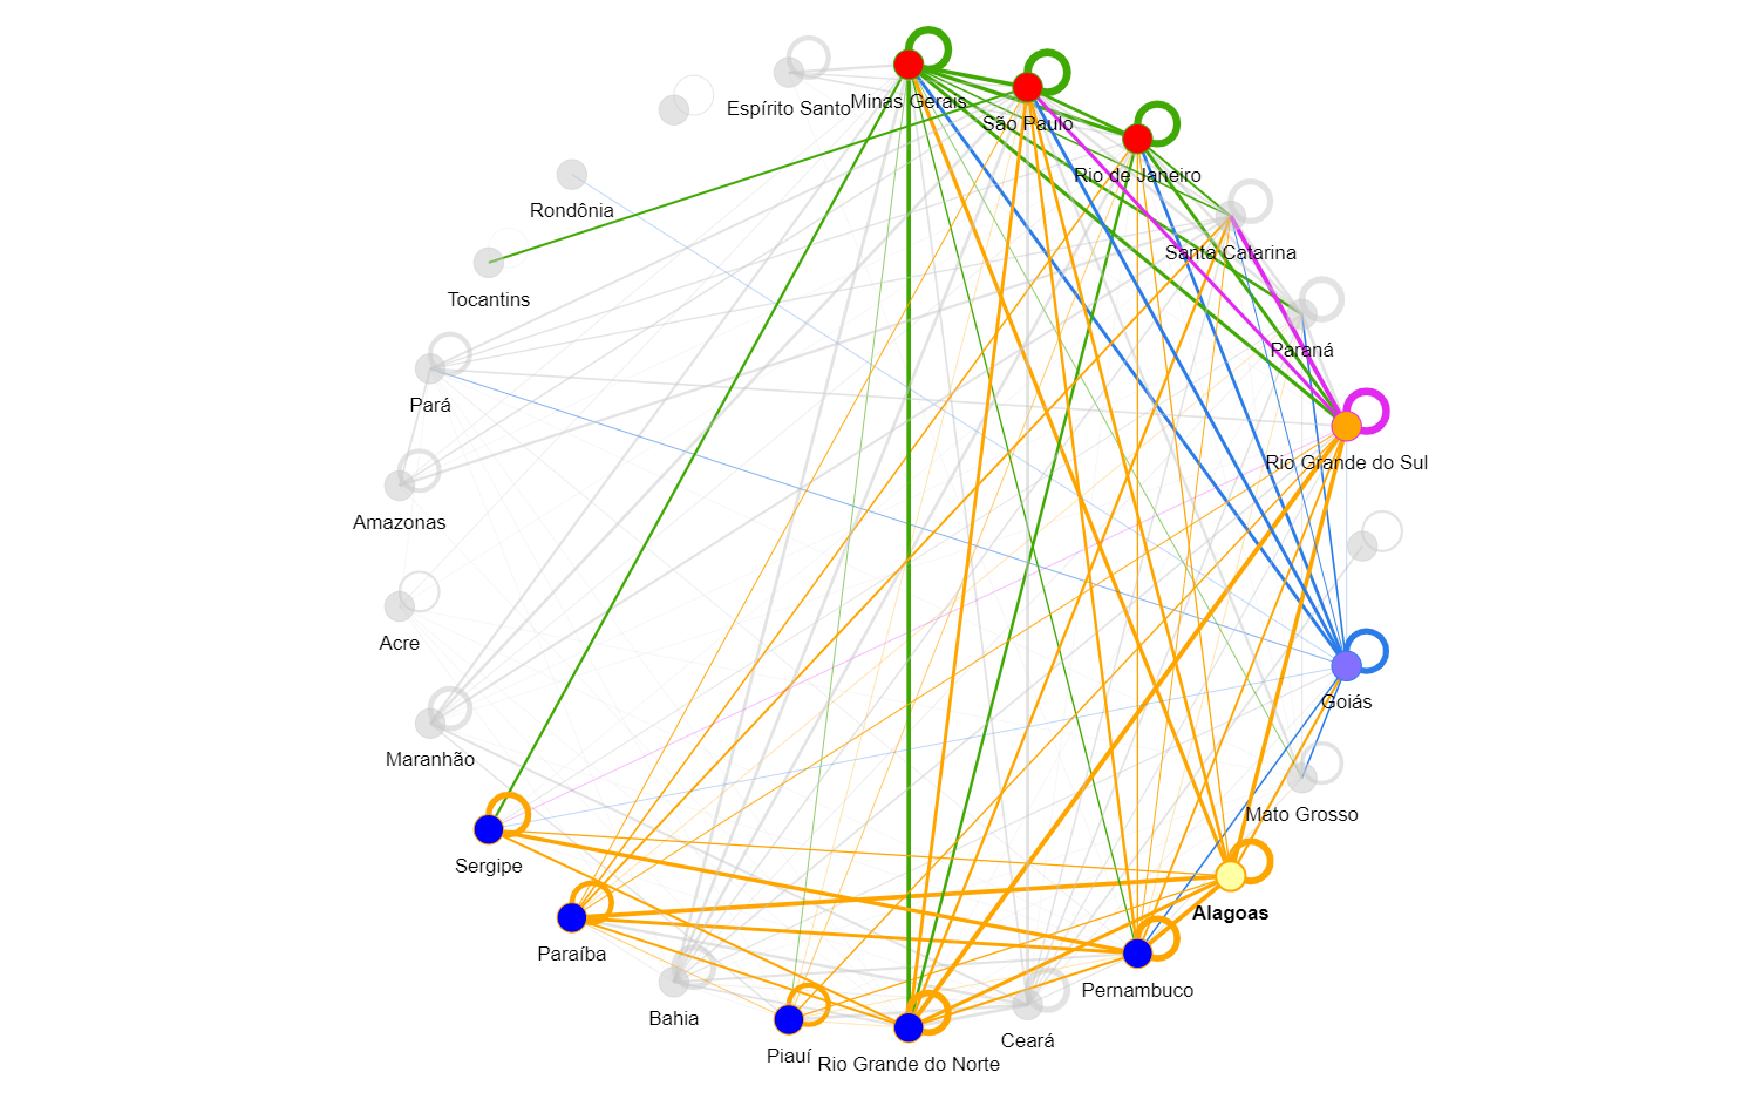
\includegraphics[width=0.38\textwidth]{images/rede-al-2011.pdf} &
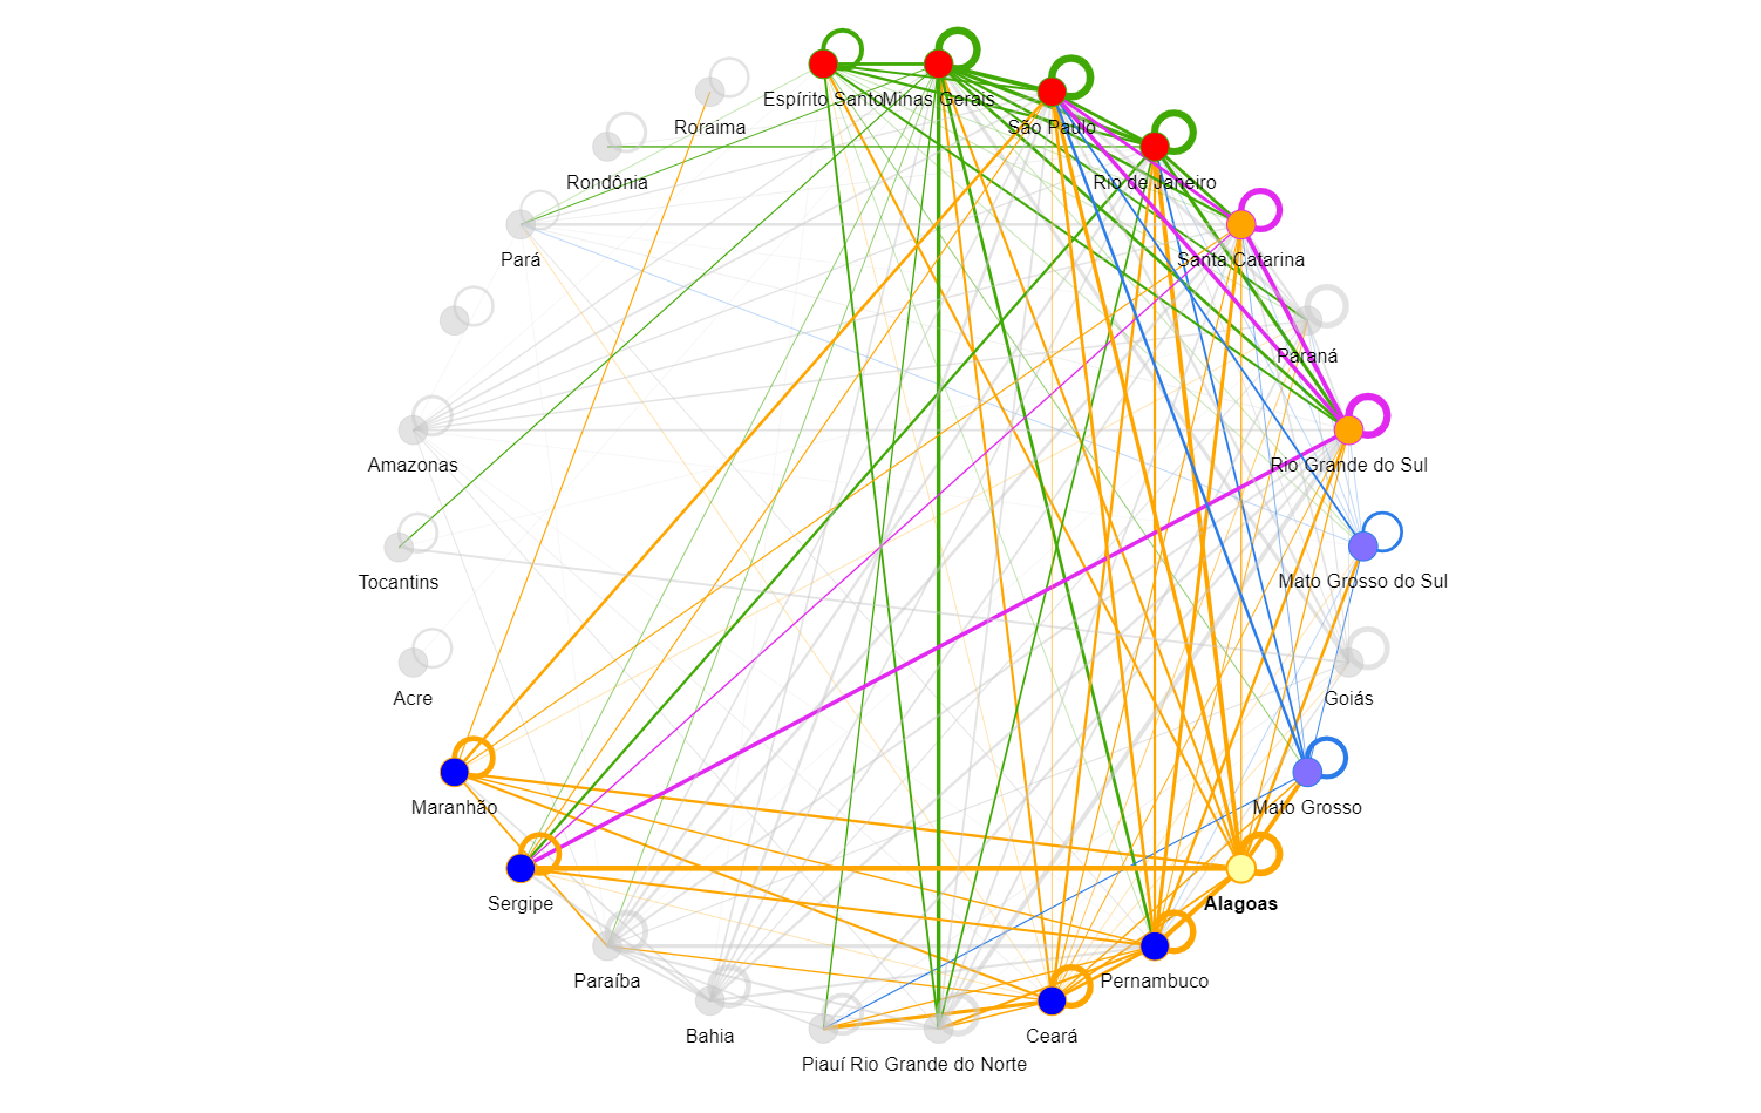
\includegraphics[width=0.38\textwidth]{images/rede-al-2012.pdf} &   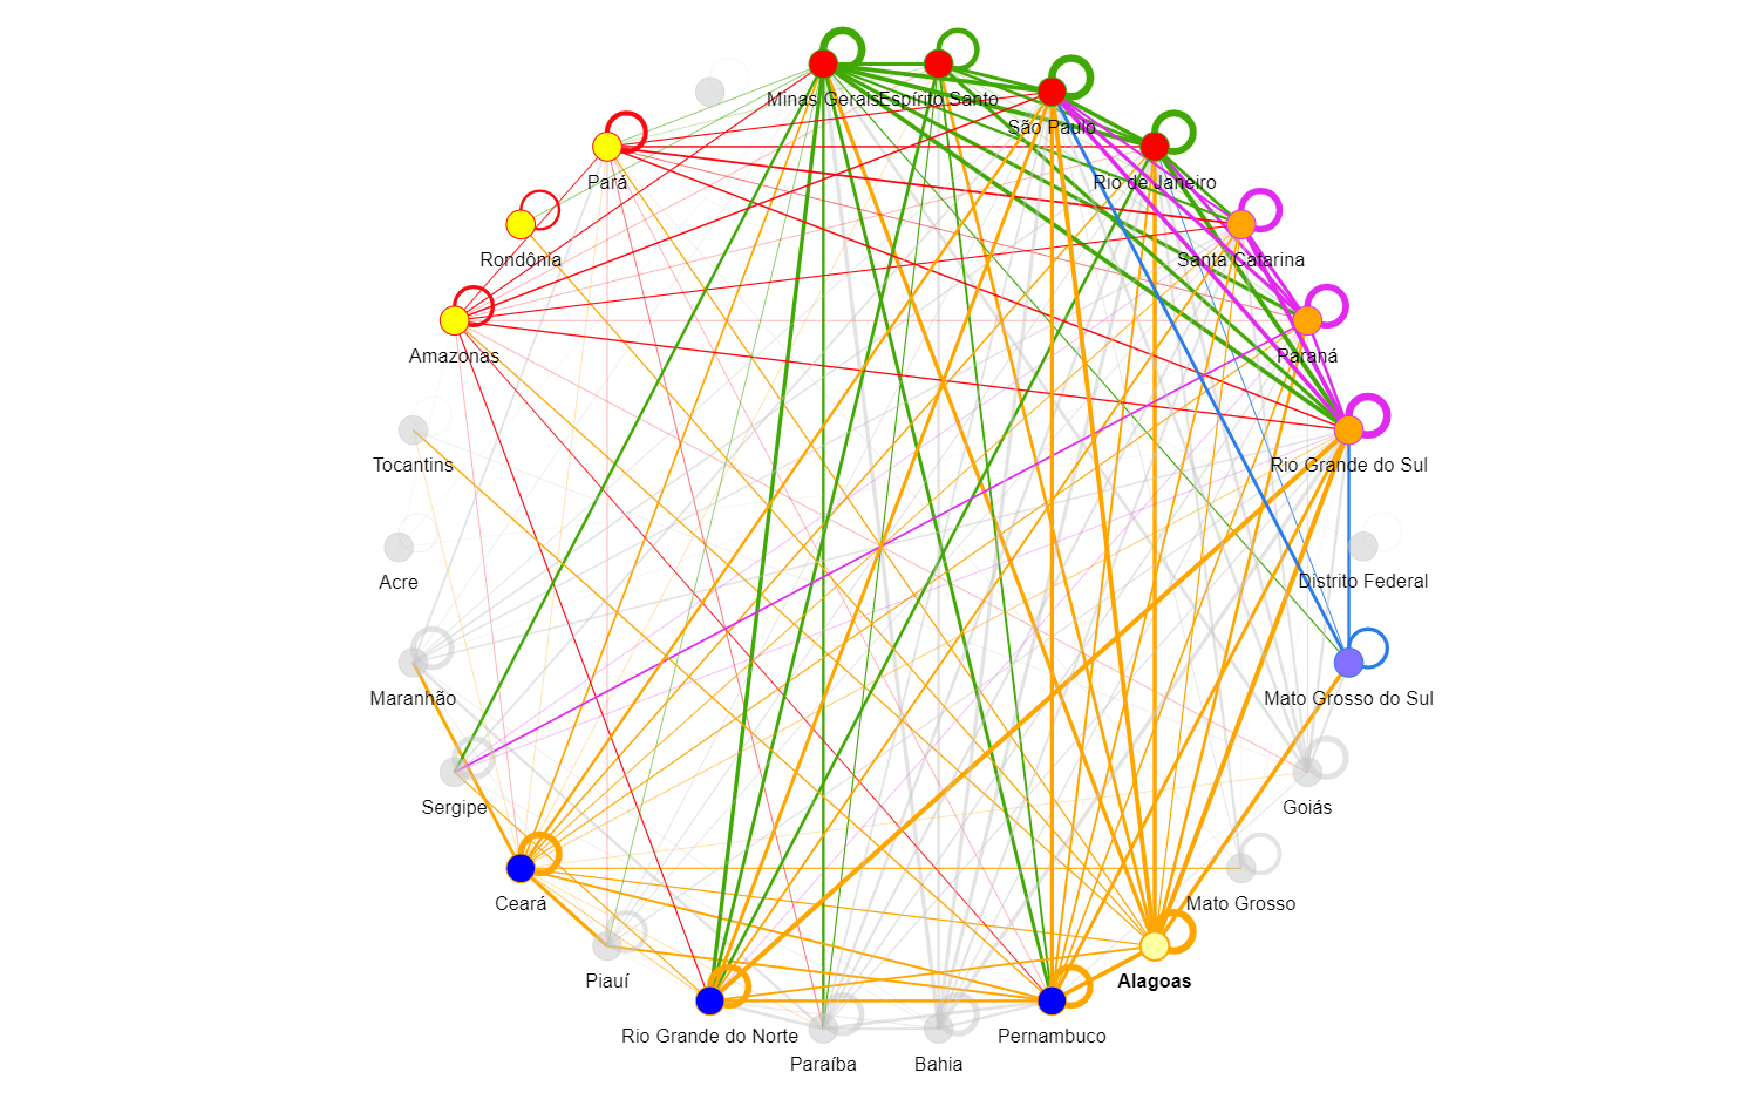
\includegraphics[width=0.38\textwidth]{images/rede-al-2013.pdf} \\
2011 & 2012 & 2013\\[6pt]
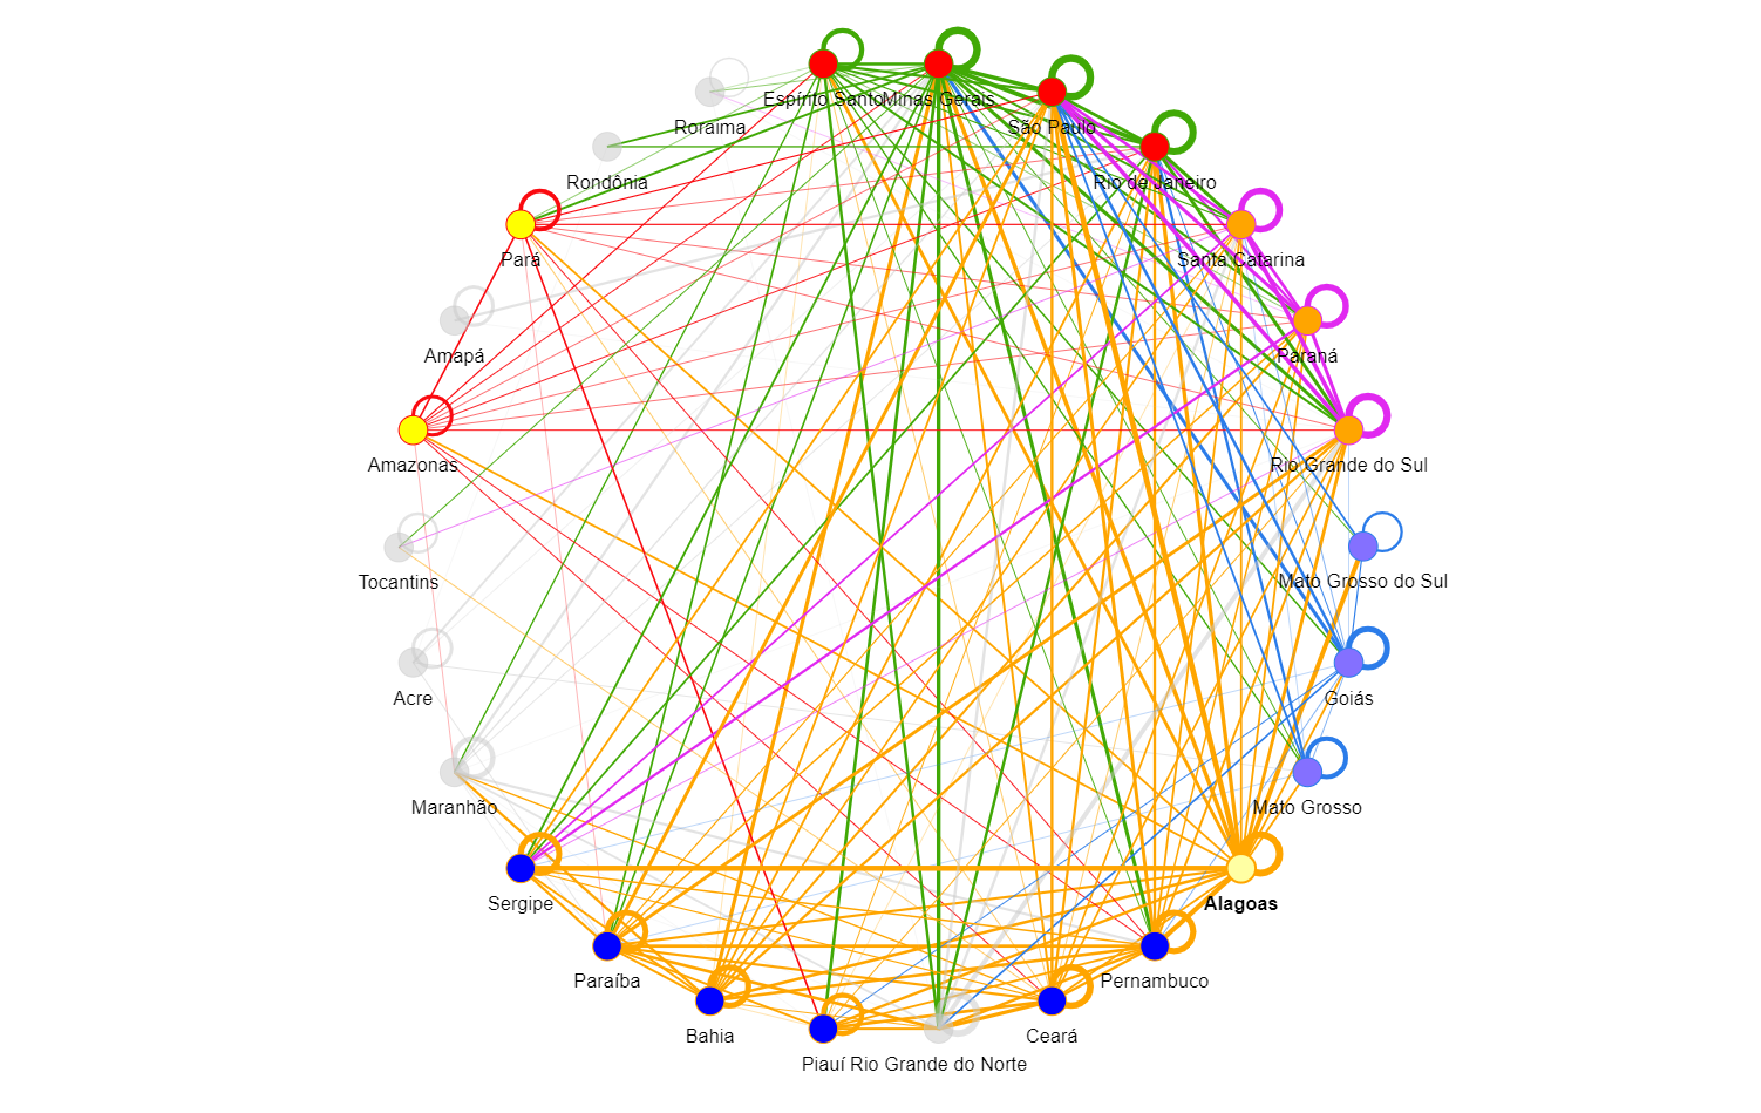
\includegraphics[width=0.38\textwidth]{images/rede-al-2014.pdf} &
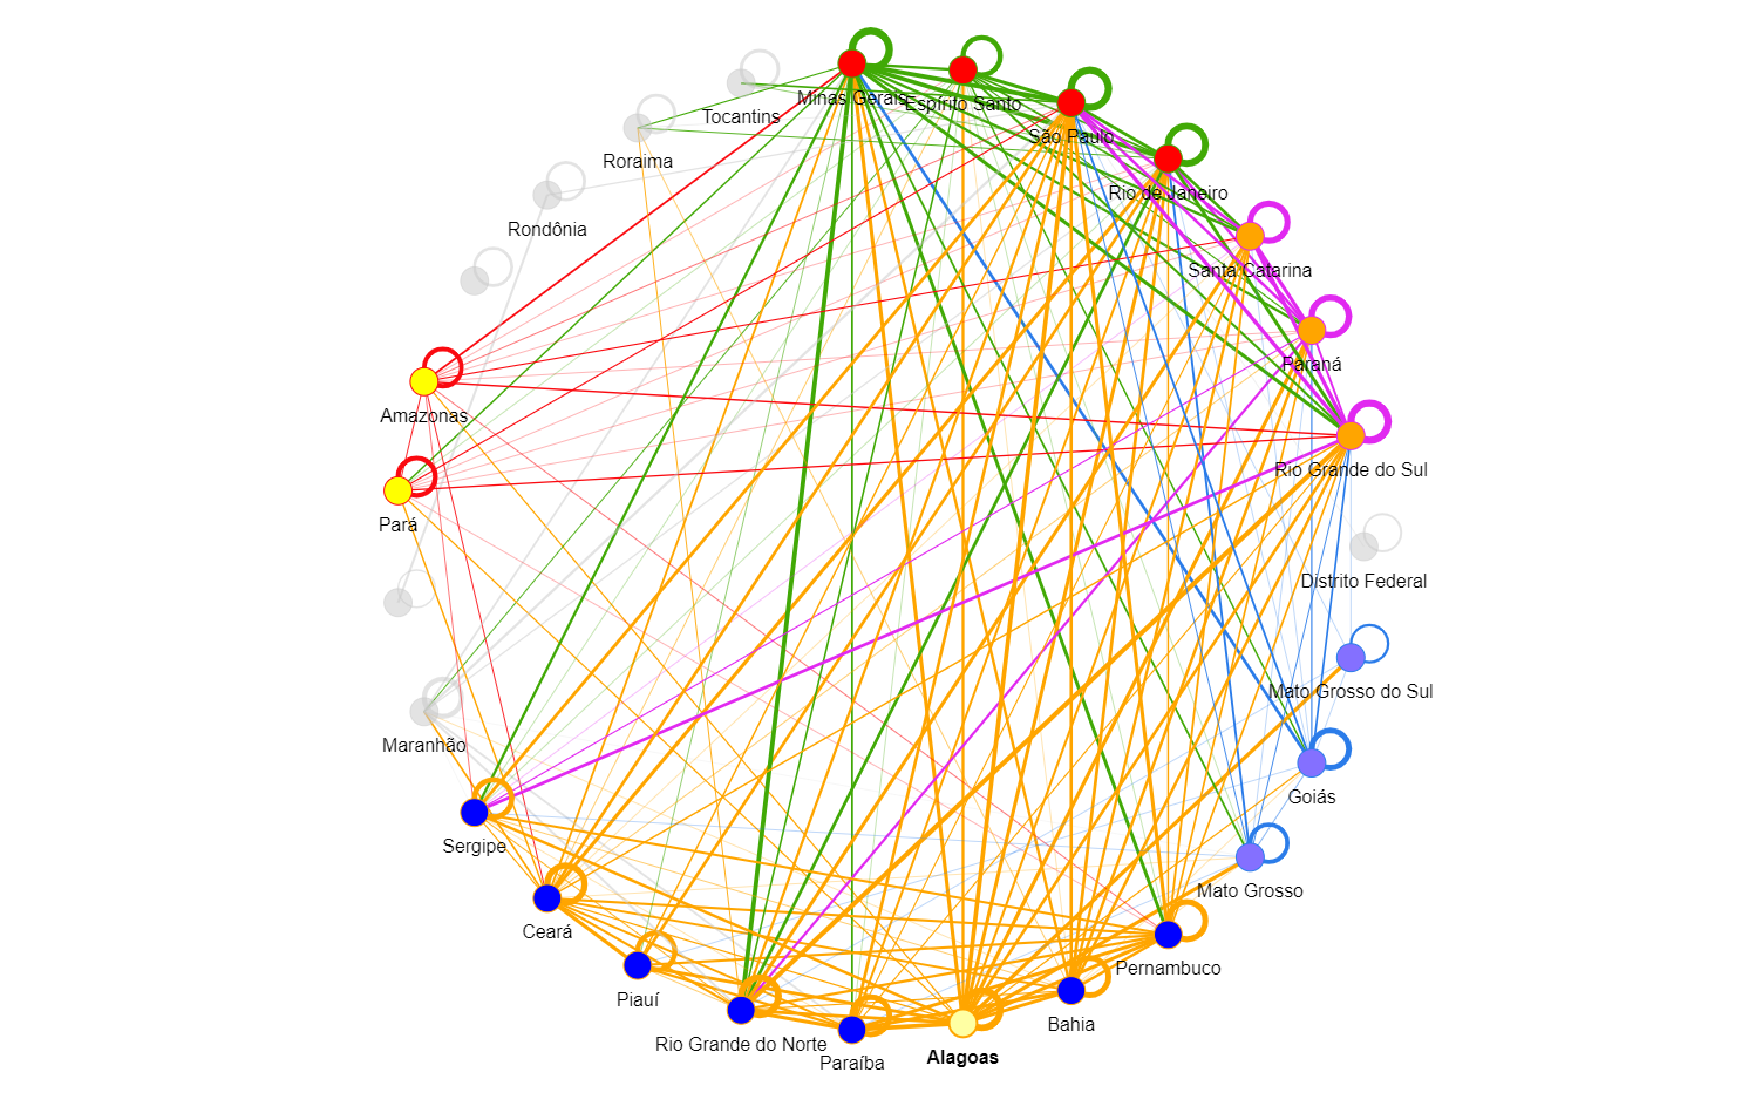
\includegraphics[width=0.38\textwidth]{images/rede-al-2015.pdf} &
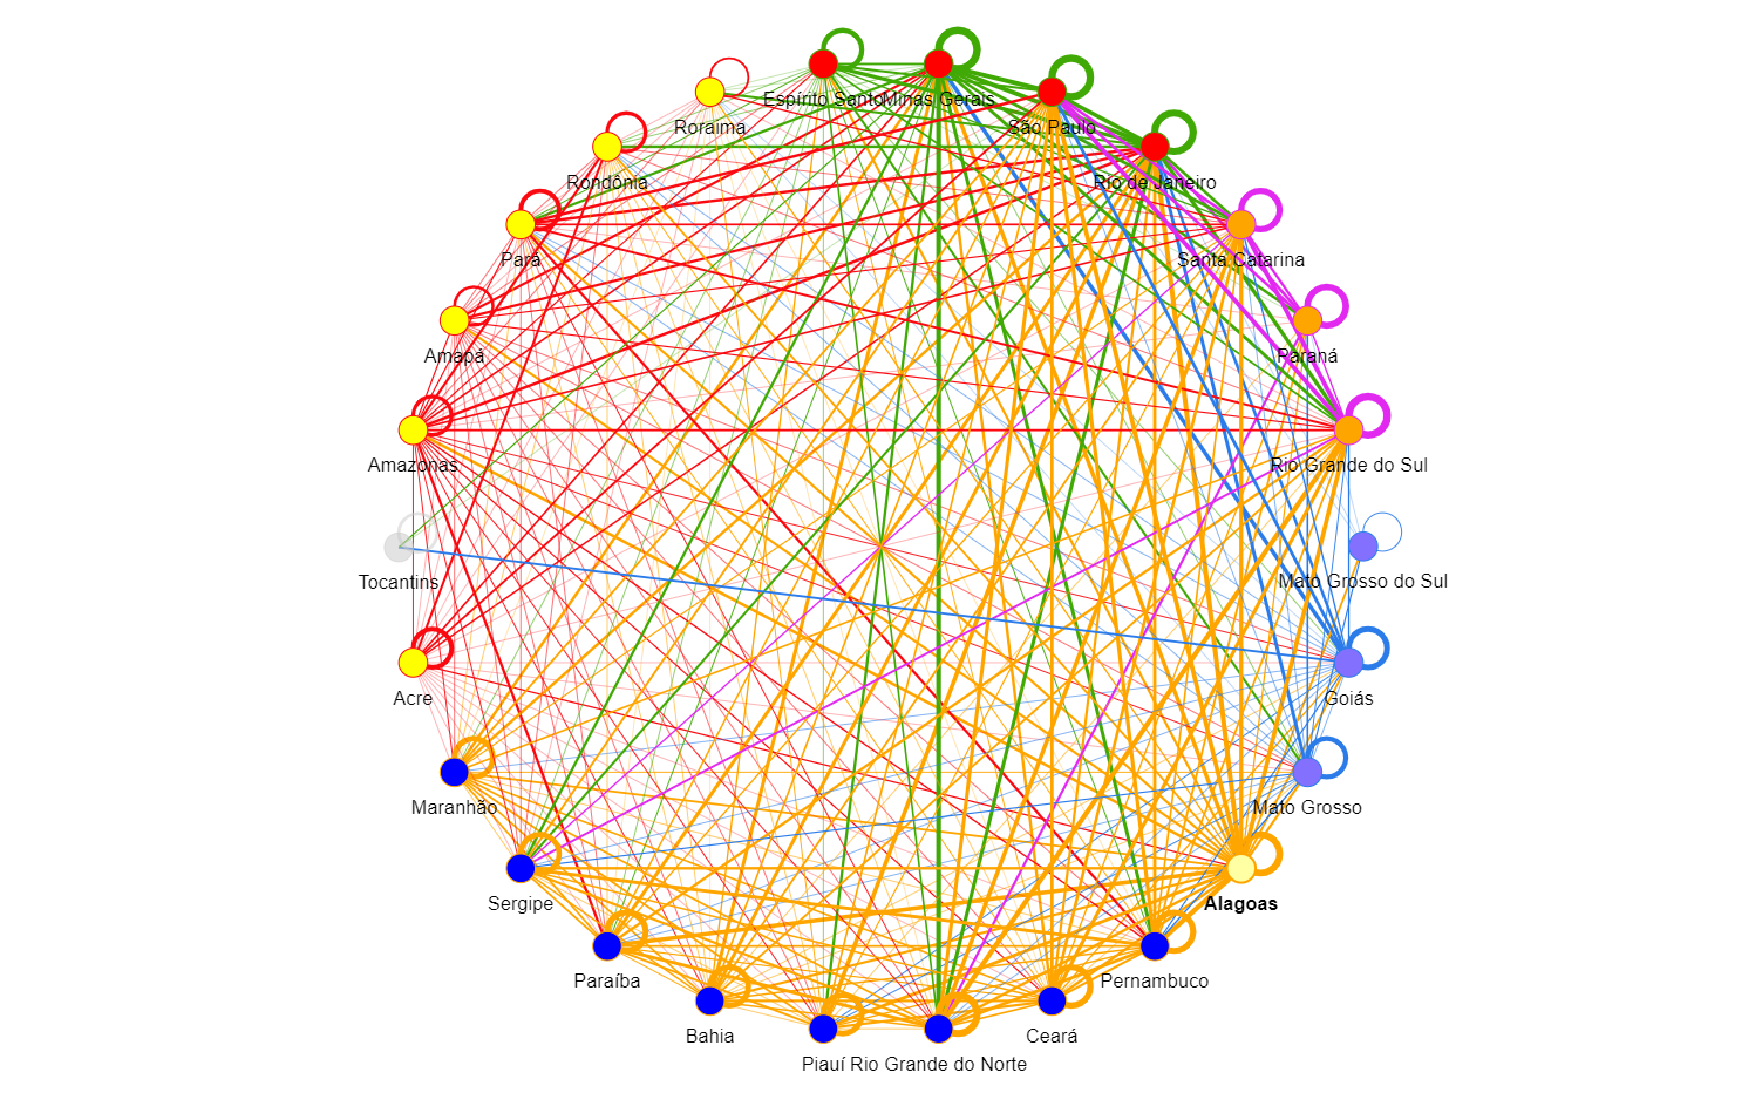
\includegraphics[width=0.38\textwidth]{images/rede-al-2016.pdf} \\
2014 & 2015 & 2016\\[6pt]  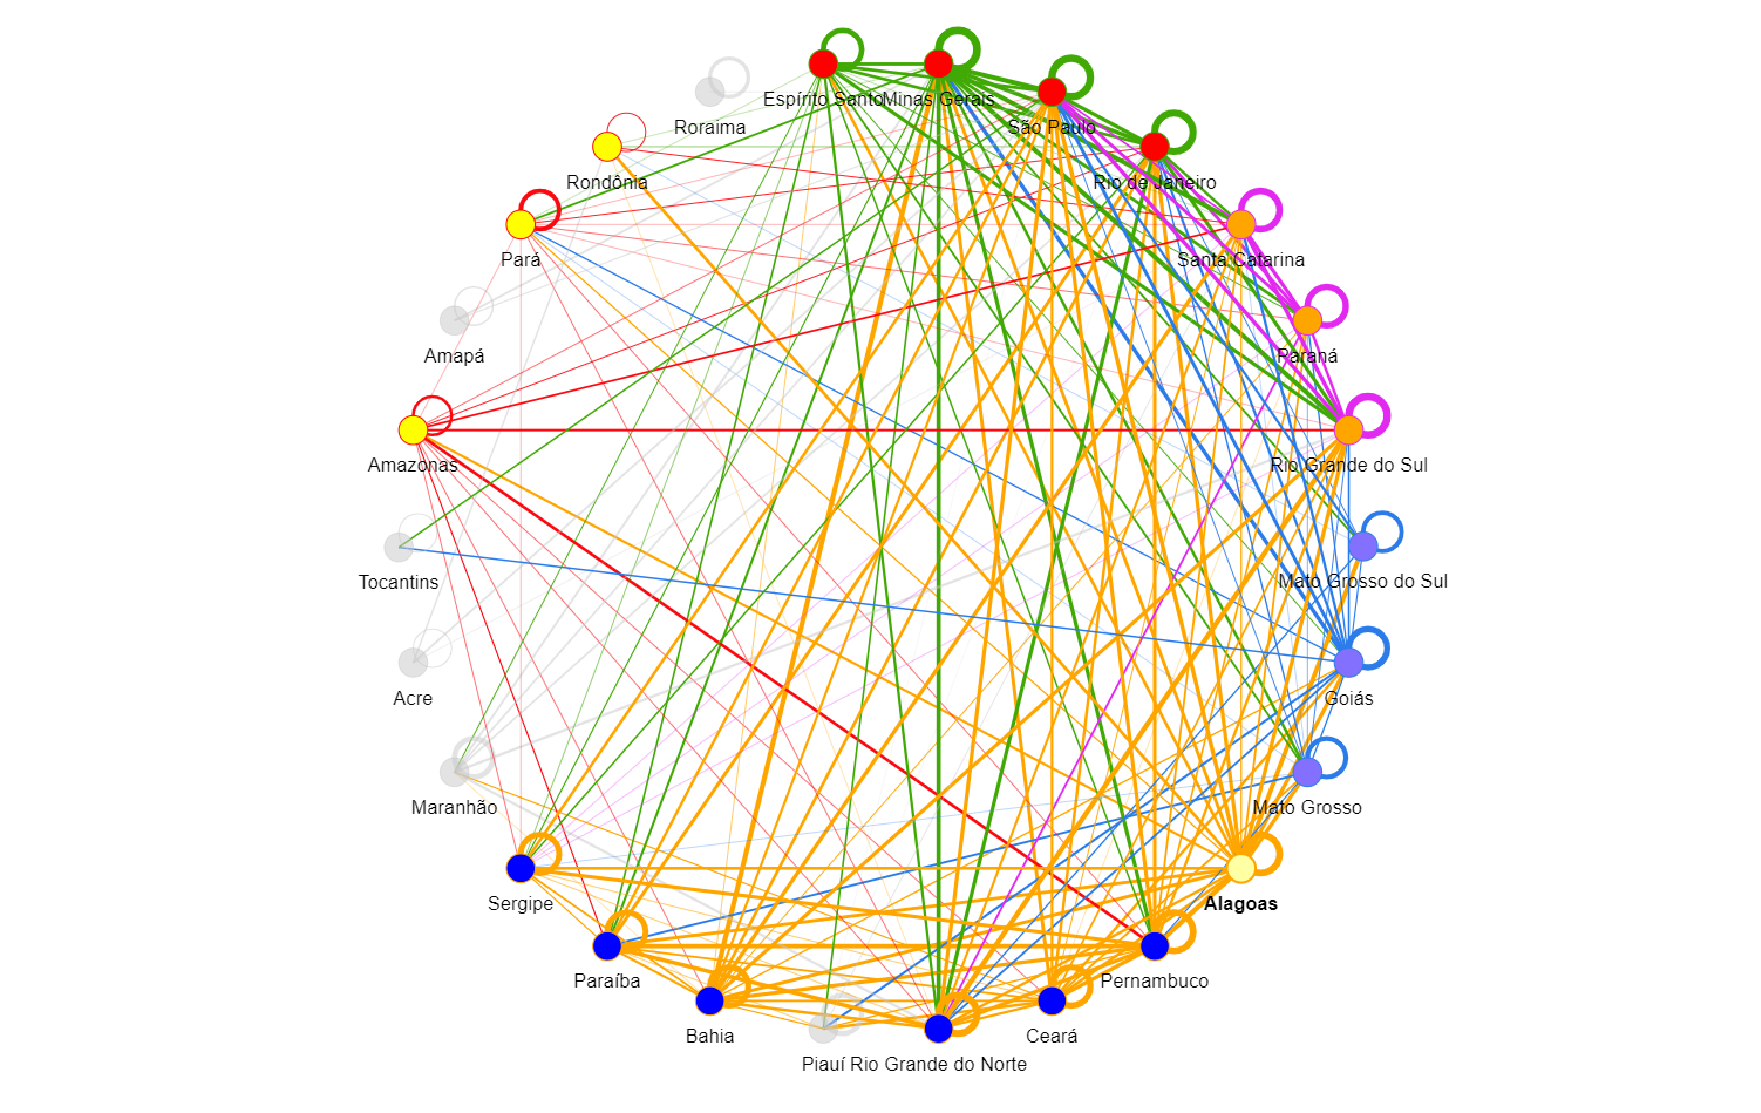
\includegraphics[width=0.38\textwidth]{images/rede-al-2017.pdf} & & \\
2017 & & \\
\end{tabular}
\caption{Redes de Coautoria da Universidade Federal de Alagoas}
\end{figure}

\subsection{Medidas de Centralidade das Redes}

A tabela abaixo apresenta o resultados das medidas de centralidade, considerando que a Rede Brasil é a média de todos os vértices da Rede de Universidades Federais do Brasil e Alagoas, a Universidade Federal de Alagoas.

A tabela abaixo apresenta os resultados das três medidas de centralidade de rede utilizada neste trabalho para a Rede Brasil e Alagoas, possibilitando a análise númerica e gráfica para a interpretação da aplicação dessas medidas para avaliação das redes de coautoria.


\begin{table}[H]
\begin{tabular}{@{}|l|l|l|l|l|l|l|@{}}
\hline
\rowcolor[HTML]{C0C0C0} 
\multicolumn{1}{|l|}{\textbf{Métrica}} & \multicolumn{2}{l|}{\textbf{\begin{tabular}[c]{@{}l@{}}Degree \\ (degree centrality)\end{tabular}}} & \multicolumn{2}{l|}{\textbf{\begin{tabular}[c]{@{}l@{}}Proximidade \\ (closeness centrality)\end{tabular}}} & \multicolumn{2}{l|}{\textbf{\begin{tabular}[c]{@{}l@{}}Intermediação \\ (betweeness centrality)\end{tabular}}} \\ 
\textbf{Ano} & \textbf{Rede Brasil} & \textbf{Alagoas} & \textbf{Rede Brasil} & \textbf{Alagoas} & \textbf{Rede Brasil} & \textbf{Alagoas}\\ 
\hline
2008 & 6,2962 &  7 & 0,5303 & 0,5434 & 0,0370 & 0,01\\ 
\hline
2009 & 7,92 & 7 & 0,5789 & 0,5609 & 0,0396 & 0,01 \\ 
\hline
2010 & 11,04 & 15 & 0,6772 & 0,7419 & 0,0388 & 0,04\\ 
\hline
2011 & 11,28 & 10 & 0,6699 & 0,6216 & 0,04 & 0,01\\ 
\hline
2012 & 11,9230 & 12 & 0,6700 & 0,6666 & 0,0380 & 0,02\\ 
\hline
2013 & 12,0769 & 14 & 0,6852 & 0,7058 & 0,0384 & 0,06\\ 
\hline
2014 & 13,2307 & 18 & 0,6957 & 0,7812 & 0,0384 & 0,05\\ 
\hline
2015 & 12,3703 & 19 & 0,6697 & 0,7812 & 0,0370 & 0,04\\ 
\hline
2016 & 20,9230 & 24 & 0,8788 & 0,9615 & 0,0396 & 0,1\\ 
\hline
2017 & 13,3076 & 19 & 0,6993 & 0,8064 & 0,0369 & 0,04\\ 
\hline
\end{tabular}
\end{table}

\subsubsection{Gráficos das Medidas de Centralidade}

\begin{figure}[H]
\centering
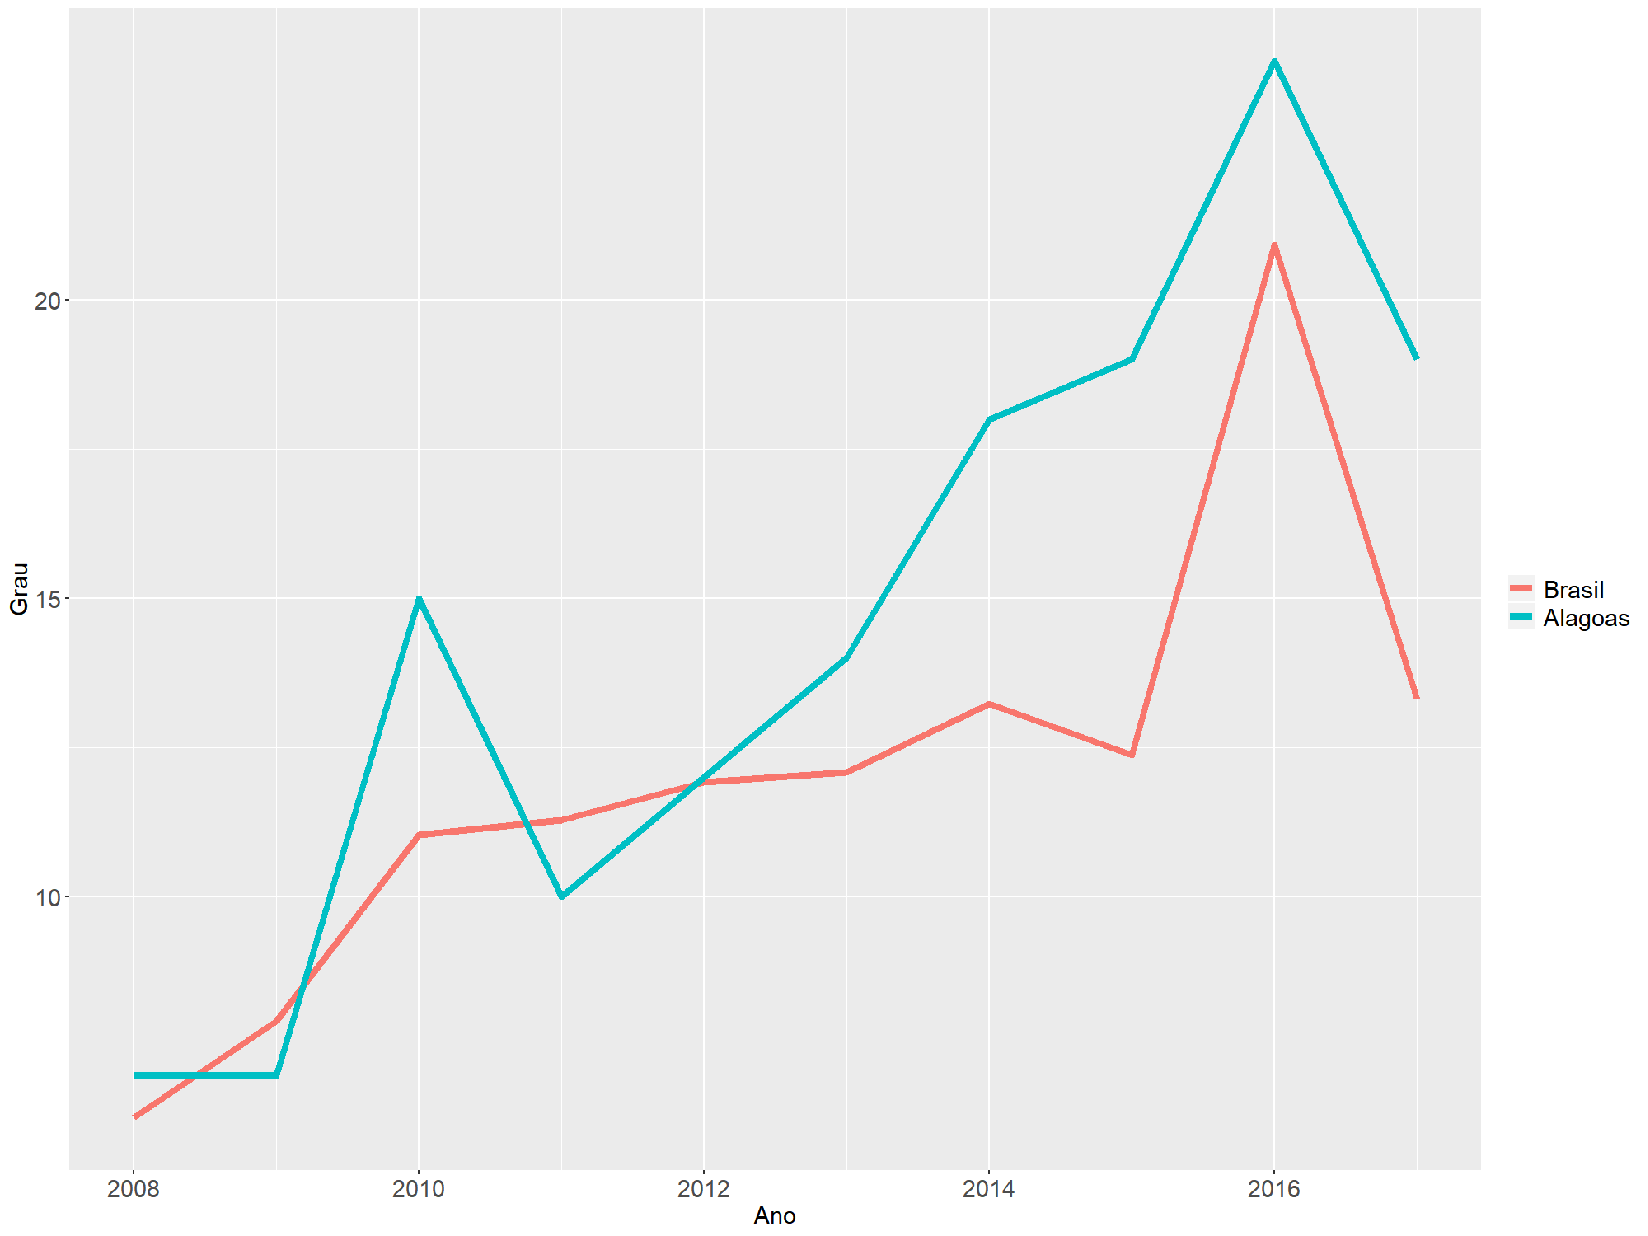
\includegraphics[scale=0.5]{images/graf-linha-degree-br-al.pdf}
\caption{Gráfico em linha - Centralidade do Grau}
%label{c}
\end{figure}

\begin{figure}[H]
\centering
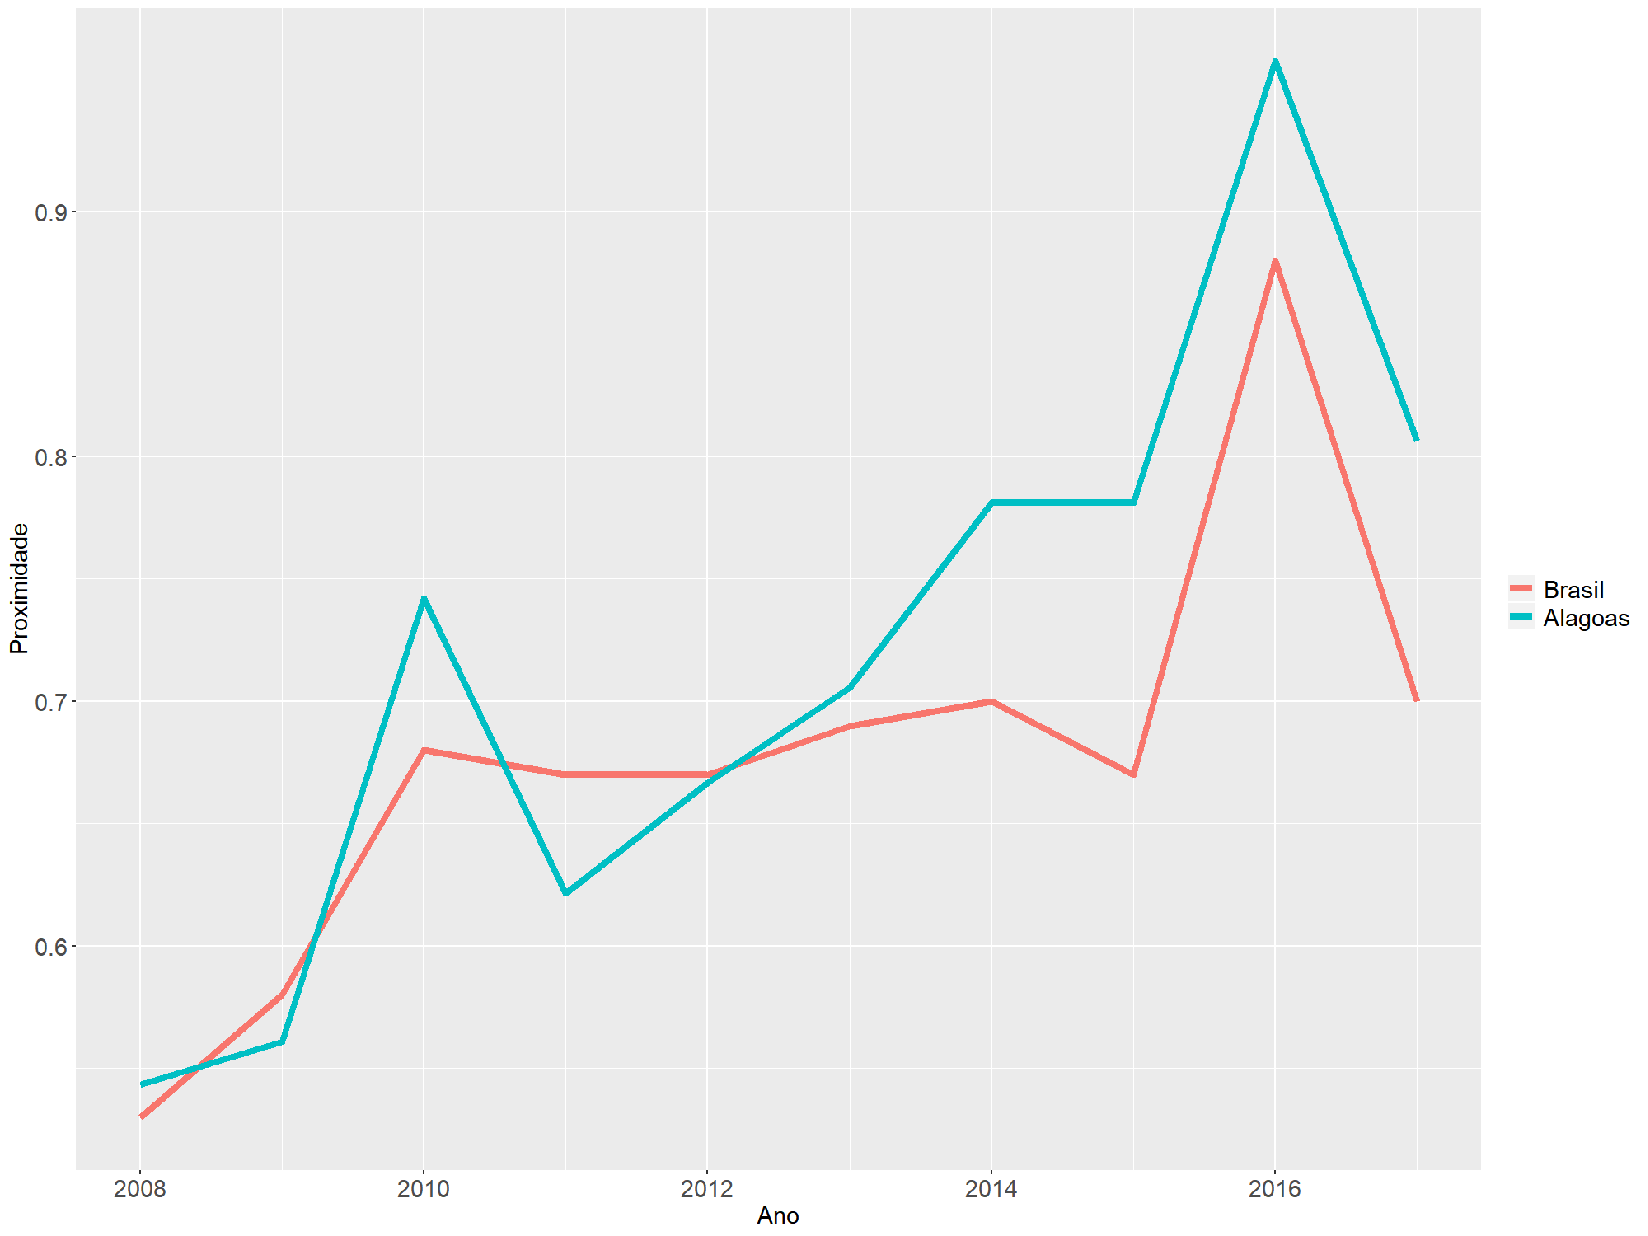
\includegraphics[scale=0.5]{images/graf-linha-closeness-br-al.pdf}
\caption{Gráfico em linha - Centralidade de Proximidade}
%label{c}
\end{figure}


\begin{figure}[H]
\centering
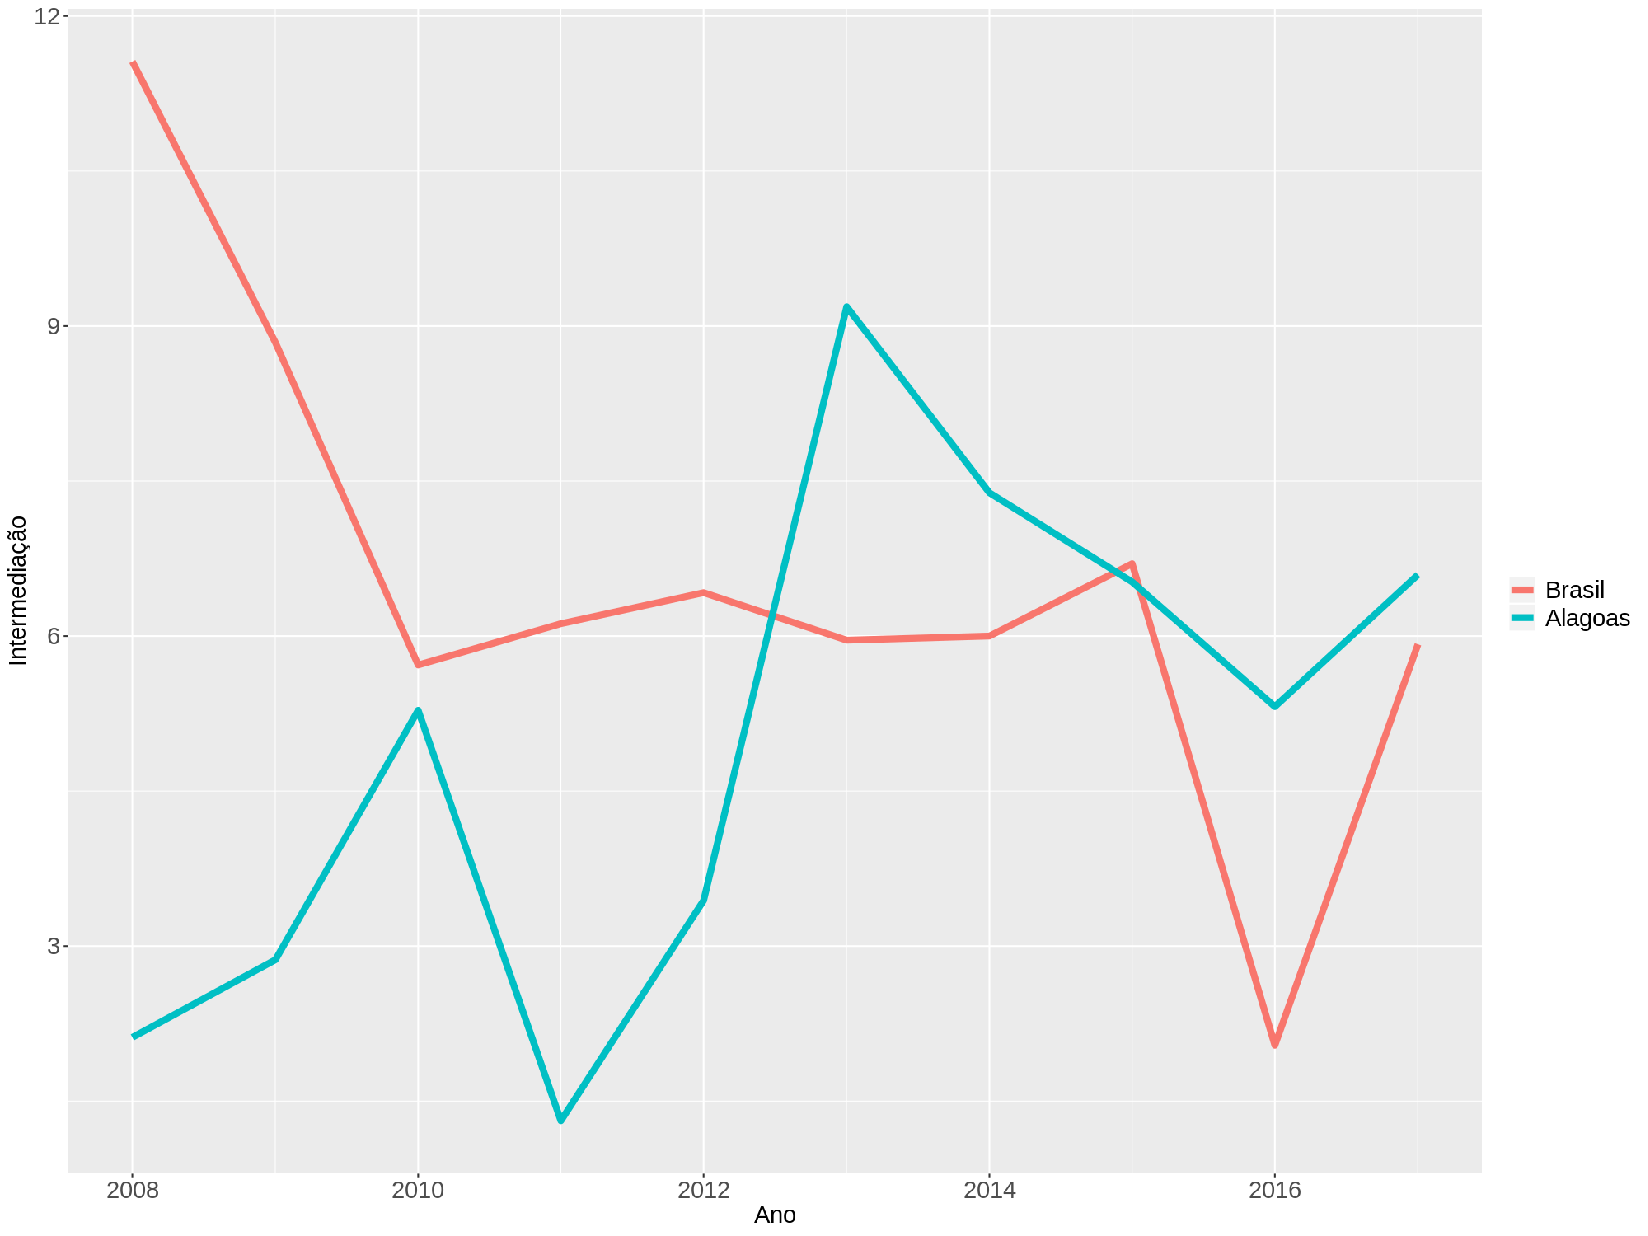
\includegraphics[scale=0.5]{images/graf-linha-betweeness-br-al.pdf}
\caption{Gráfico em linha - Centralidade de Intemediação}
\label{c2}
\end{figure}

As curvas dos gráficos de Centralidade do Grau e Centralidade de Proximidade se projetaram de forma muito parecidas, mostrando então que Alagoas acompanhou as medidas médias da Rede Brasil, o que não se observou na curva do gráfico de Centralidade de Intermediação, uma vez que, já no primeiro ano mostra uma grande diferença para esta medida, tendo um pico crescente no de 2013, mostrando que a influência de intermediação de Alagoas foi maior que a média da Rede Brasil.

\subsubsection{Histograma das Medidas de Centralidade}

Os histogramas das frequência das medidas, foram plotados permitindo observar o posionamento de Alagoas e da Rede Brasil nas distribuições de cada medida.

\begin{figure}[H]
\centering
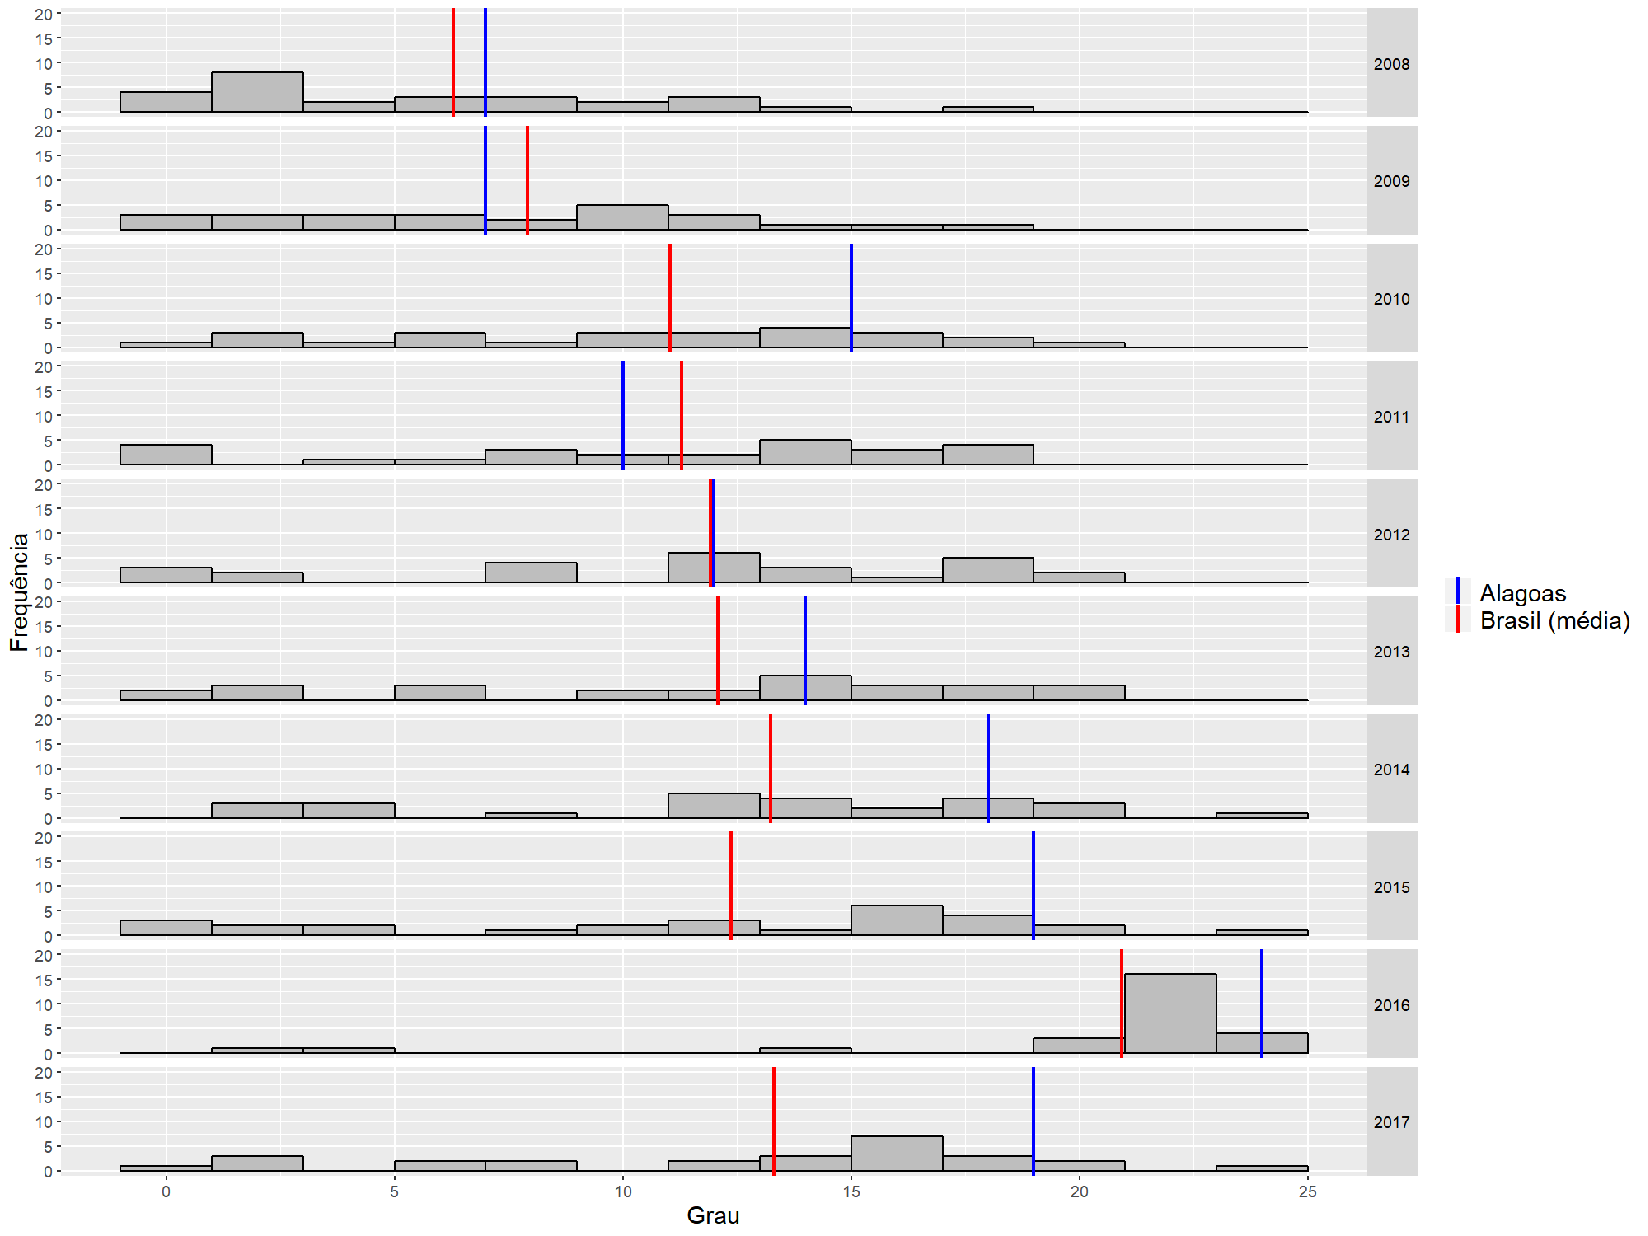
\includegraphics[scale=0.6]{images/degree-hist.pdf}
\caption{Histograma da Centralidade do Grau \textit{(degree centrality)}}
%label{c}
\end{figure}

\begin{figure}[H]
\centering
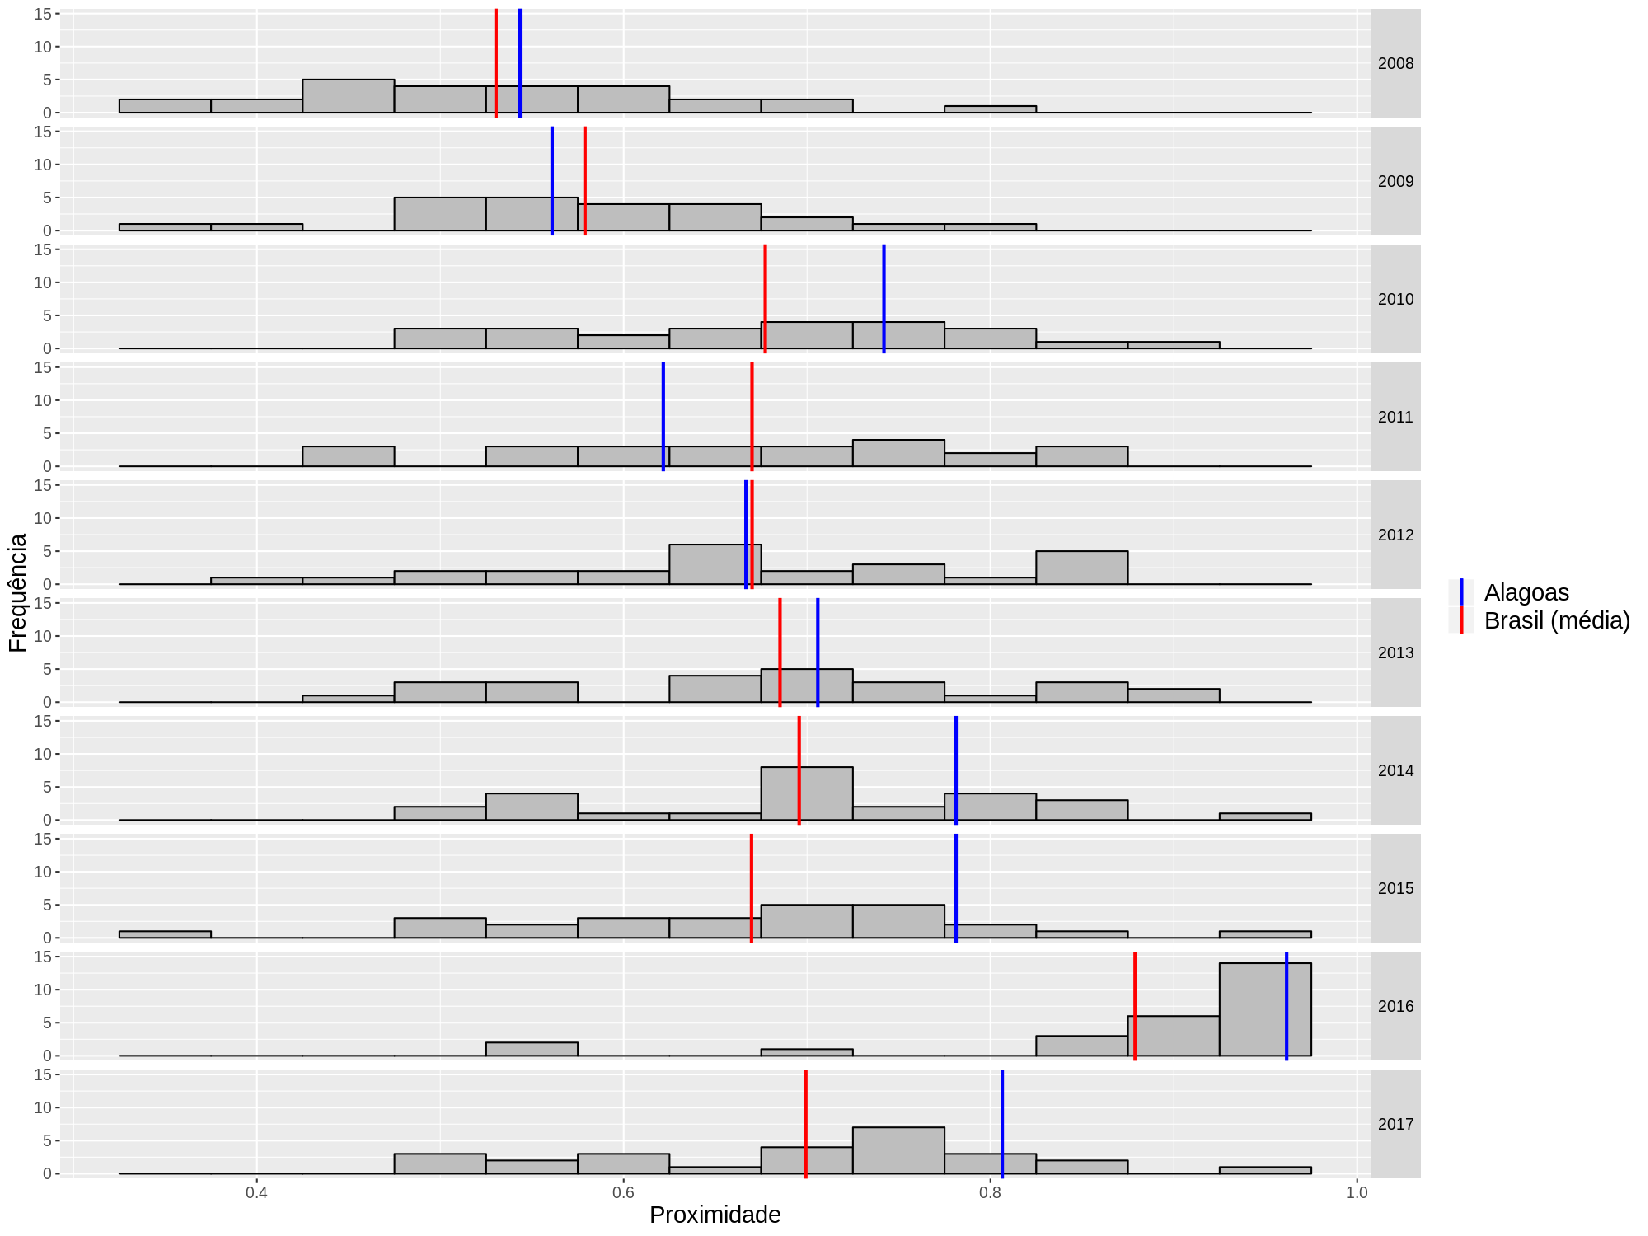
\includegraphics[scale=0.6]{images/closeness-hist.pdf}
\caption{Histograma da Centralidade de Proximidade \textit{(closeness centrality)}}
%label{c}
\end{figure}

\begin{figure}[H]
\centering
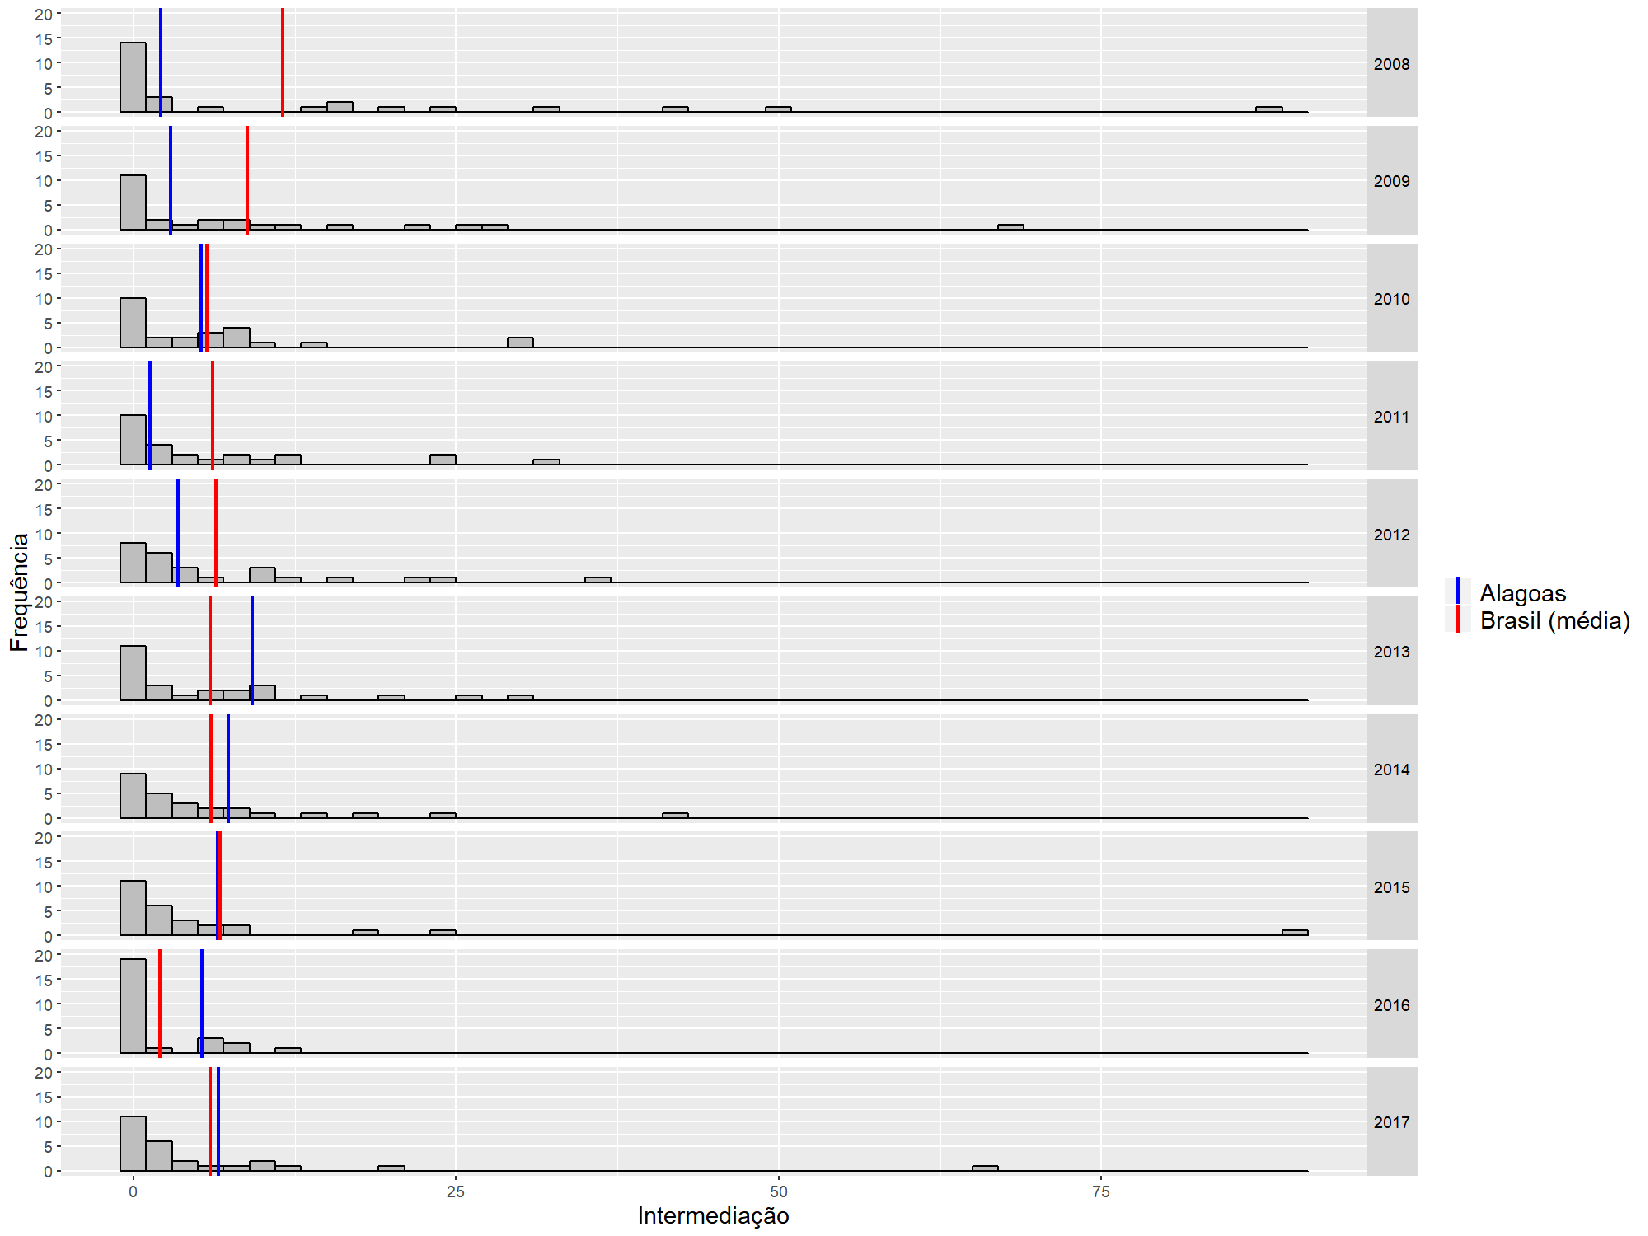
\includegraphics[scale=0.6]{images/betweeness-hist.pdf}
\caption{Histograma da Centralidade de Intermediação \textit{(betweeness centrality)}}
\label{c22}
\end{figure}

\section{Conclusões}

A seguir apresentamos nossas considerações finais, buscando a contextualização do problema de pesquisa em tela e os resultados obtidos com o presente trabalho de pesquisa.

\subsection{Considerações Finais}

Com a proposta apresentada, buscamos destacar a importância do estudo de redes de coautorias relacionando ao acabouço teórico de redes complexas e a relação com a colaboração científica, neste trabalho a compreensão da interação existente entre as Universidades Federais do Brasil e a Universidade Federal de Alagoas.

Conforme \citep{barabasi2002evolution}, os estudos de redes de coautoria são importantes e possuem sua relevância para apresentar padrões de comportamento e possibilitar modelos preditivos de quais áreas ou campos estão se desenvolvendo, são emergentes, ou quais tendências poussuem.

O estudo das redes de coautoria deste trabalho, mostrou um resultado que se aplicado a outras redes poderão descrever o comportamento, dinâmica e características, quando se observa as relações existentes dentro de uma área \textit{Health Sciences}, a partir da consideração de uma base de indexação de artigoes específica ou de outra.

As medidas de centralidade possibilitam aferir conhecimento a respeito da dinâmica e do comportamento das redes de coautorias no aspecto temporal. A aplicação destas, em outras áreas do conhecimento e em outras bases de indexação de artigos científicos, mostram-se significativas para a obtenção de resultados específico para avaliação da colaboração científica, possibilitando a compreensão e caracterização dos atores de relevância e influência da rede.

\subsection{Trabalhos Futuros}

Por trabalhos futuros, partindo da consideração da expansão do uso de outras medidas de centralidade de rede, para a análise topólogica, outras abordagens de uma prisma analítico e probabilístico, podemos sugerir a utlização de técnicas de \textit{network-driven approaches} como \textit{link prediction}, análise de comunidades de influências na rede, e simulação do comportamento da rede com base em métricas de redes complexas.

\bibliographystyle{apalike}
\nocite{*}
\bibliography{references}

\end{document}
